% * select [german] or [english]
% * use option "alpha" for abbreviated citation (instead of numbers)
% * option "draft" is available, too
\documentclass[german]{thesis_KBS}

\usepackage[utf8]{inputenc}
\usepackage{hyphenat}
\usepackage{units}    % useful for settings units, \unit[23]{m}
\usepackage{nicefrac} % for setting fractions esp. within text, \nicefrac{km}{h}
\usepackage{pdfpages}
\usepackage{graphicx}
\usepackage{wrapfig}
%\usepackage{xparse}
%\usepackage{xstring}
\usepackage{framed}
\usepackage{keystroke}
\usepackage{listings}
\usepackage{lstautogobble}
\usepackage{url}
\usepackage[pdfborder={0 0 0}]{hyperref}
\usepackage{pgfplots}
\usepackage{tikz}
\usetikzlibrary[
    shapes.misc,shapes.geometric,shapes.multipart,arrows,matrix,fit,
    decorations.pathmorphing,backgrounds,fit,positioning,patterns
]

\lstset{
    float=tb,
    numbers=left,
    basicstyle=\ttfamily\small, 		% Setzt den Standardstil
    keywordstyle=\color{blue}\bfseries\small, 		% Setzt den Stil für Schlüsselwörter
    identifierstyle=\bfseries, 		% Identifier fett
    tabsize=4,				% Breite der Tabs
    showstringspaces=false,			% Leerzeichen in Strings nicht anzeigen
    commentstyle=\color{red!50}, 		% Stil für Kommentare
    stringstyle=\color{blue!50}, 		% Stil für Strings (gekennzeichnet mit "String")
    breaklines=true, 			% Zeilen werden umgebrochen
    numbers=left, 				% Zeilennummern links
    numberstyle=\tiny, 			% Stil für die Seitennummern
    frame=single, 				% Rahmen
    backgroundcolor=\color{black!10}, 	% Hintergrundfarbe
    captionpos=b,				% Position der Listingunterschrift
    autogobble
}

%%%%%%%%%%%%%%%%%%%%%%%%%%%%%%%%%%%%%
% YAML highlighting
%%%%%%%%%%%%%%%%%%%%%%%%%%%%%%%%%%%%%
\newcommand\YAMLcolonstyle{\color{red}\ttfamily}
\newcommand\YAMLkeystyle{\color{black}\ttfamily}
\newcommand\YAMLvaluestyle{\color{blue}\ttfamily}

\makeatletter

% here is a macro expanding to the name of the language
% (handy if you decide to change it further down the road)
\newcommand\language@yaml{yaml}

\expandafter\expandafter\expandafter\lstdefinelanguage
\expandafter{\language@yaml}
{
  keywords={true,false,null,y,n},
  keywordstyle=\color{darkgray}\ttfamily,
  basicstyle=\YAMLkeystyle,                                 % assuming a key comes first
  sensitive=false,
  comment=[l]{\#},
  morecomment=[s]{/*}{*/},
  commentstyle=\color{purple}\ttfamily,
  stringstyle=\YAMLvaluestyle\ttfamily,
  moredelim=[l][\color{orange}]{\&},
  moredelim=[l][\color{magenta}]{*},
  moredelim=**[il][\YAMLcolonstyle{:}\YAMLvaluestyle]{:},   % switch to value style at :
  morestring=[b]',
  morestring=[b]",
  literate =    {---}{{\ProcessThreeDashes}}3
                {>}{{\textcolor{red}\textgreater}}1
                {|}{{\textcolor{red}\textbar}}1
                {\ -\ }{{\mdseries\ -\ }}3,
}

% switch to key style at EOL
\lst@AddToHook{EveryLine}{\ifx\lst@language\language@yaml\YAMLkeystyle\fi}
\makeatother

\newcommand\ProcessThreeDashes{\llap{\color{cyan}\mdseries-{-}-}}


% Defines the \replace command from https://tex.stackexchange.com/a/213950
% Usage: \replace{haystack}{needle}{replacement}
\def\replace#1#2#3{%
 \def\tmp##1#2{##1#3\tmp}%
   \tmp#1\stopreplace#2\stopreplace}
\def\stopreplace#1\stopreplace{}

%%%%%%%%%%%%%%%%%%%%%%%%%%%%%%%%%%%%%%%%%%%%%%%%%%%%%%%%%
%%% Ein paar Hilfskommandos, die nützlich sein können %%%
%%%%%%%%%%%%%%%%%%%%%%%%%%%%%%%%%%%%%%%%%%%%%%%%%%%%%%%%%

% \textsf = sans-serif font
% \texttt = type writer style font
\newcommand{\code}[1]{\texttt{#1}}  % Code in Text

%%%%%%%%%%%%%%%%%%%%%%%%%%%%%%%%%%%%%%%%%%%%%%%%%%%%%%%%%%%%%%%%%%%%%%%%%%%%%%%%%%%%

\begin{document}

\title{Bau und Implementierung einer Steuerungseinheit für einen KURT2 Roboter mithilfe eines Raspberry Pis}
\type{Bachelorarbeit}                  % by default Masterarbeit / Master's Thesis
%\dept{...}                             % by default KBS UOS
%\submitdate{November 2004}             % by default current month & year
%\signcity{}                            % by default Osnabrück
%signline{Osnabrück, 11. Dezember 2004} % by default "signcity, submitdate"
\author{Jonas Schievink}
\email{jschievink@uni-osnabrueck.de}
\firstSupervisor{Prof. Dr. Joachim Hertzberg}
\secondSupervisor{Dr. Thomas Wiemann}


\generatetitle

\cleardoublepage

\begin{prefacesection}{Zusammenfassung}
Die vorliegende Arbeit entwickelt eine Hard- und Softwarelösung zur Steuerung
eines KURT2-Roboters. Ein Einplatinencomputer vom Typ Raspberry Pi 2 Model B
wird verwendet, um die Software auszuführen und direkt mit der Hardware zu
kommunizieren. Die zusätzlich benötigte Elektronik wird auf ein Minimum
beschränkt und kein externer Mikrocontroller ist erforderlich. Die Erzeugung der
benötigten Steuerungssignale für die Motoren wird von der
\code{pigpio}-Bibliothek übernommen.

Die Motortreiber des alten KURT2-Roboters werden weitergenutzt und analysiert,
da keine Datenblätter oder Schaltpläne vorlagen. Ein vereinfachter Schaltplan
wird angelegt und die elektrischen Eigenschaften charakterisiert.

Der Raspberry Pi kann mittels LAN in ein lokales Roboternetzwerk integriert
werden und führt die Regelung der Motorgeschwindigkeit sowie die Auswertung der
Encodersignale durch. Die Software basiert auf dem Robot Operating System (ROS)
und implementiert die von ROS genutzten Standardschnittstellen, wodurch
bestehende Anwendungen mit minimalen Änderungen weiterverwendet werden können.
Der Code wurde umfangreich dokumentiert, um auch für Neulinge zugänglich zu sein
und um Wartung und Erweiterung der Software zu vereinfachen. Zusätzlich zu der
hier vorgestellten Software können weitere Komponenten auf dem Raspberry Pi
ausgeführt werden, die andere Aufgaben übernehmen und überschüssige CPU-Zeit
beanspruchen können.
\end{prefacesection}

\cleardoublepage
\tableofcontents


\startTextChapters

%\unit[23]{m}
% \nicefrac{km}{h}

\chapter{Einleitung}

Das Ziel dieser Arbeit ist, die veraltete Elektronik eines KURT2-Roboters
auszutauschen und zu modernisieren, sowie eine neue Steuerungssoftware dafür zu
schreiben.

Die Elektronik soll dabei so simpel wie möglich gehalten werden und gut
dokumentiert werden, um Wartung und spätere Modifikation zu vereinfachen. Auch
die Softwarekomponenten sollen gut dokumentiert und wartungsfreundlich gestaltet
werden.

Um Motivation und Ziel dieser Arbeit genau festzulegen, soll zuerst die
KURT2-Roboterplattform sowie die Raspberry Pi Plattform genauer beschrieben
werden.


\section{KURT2}

\begin{wrapfigure}[16]{r}{0.35\textwidth}
    \vspace{-12pt}
    \centering 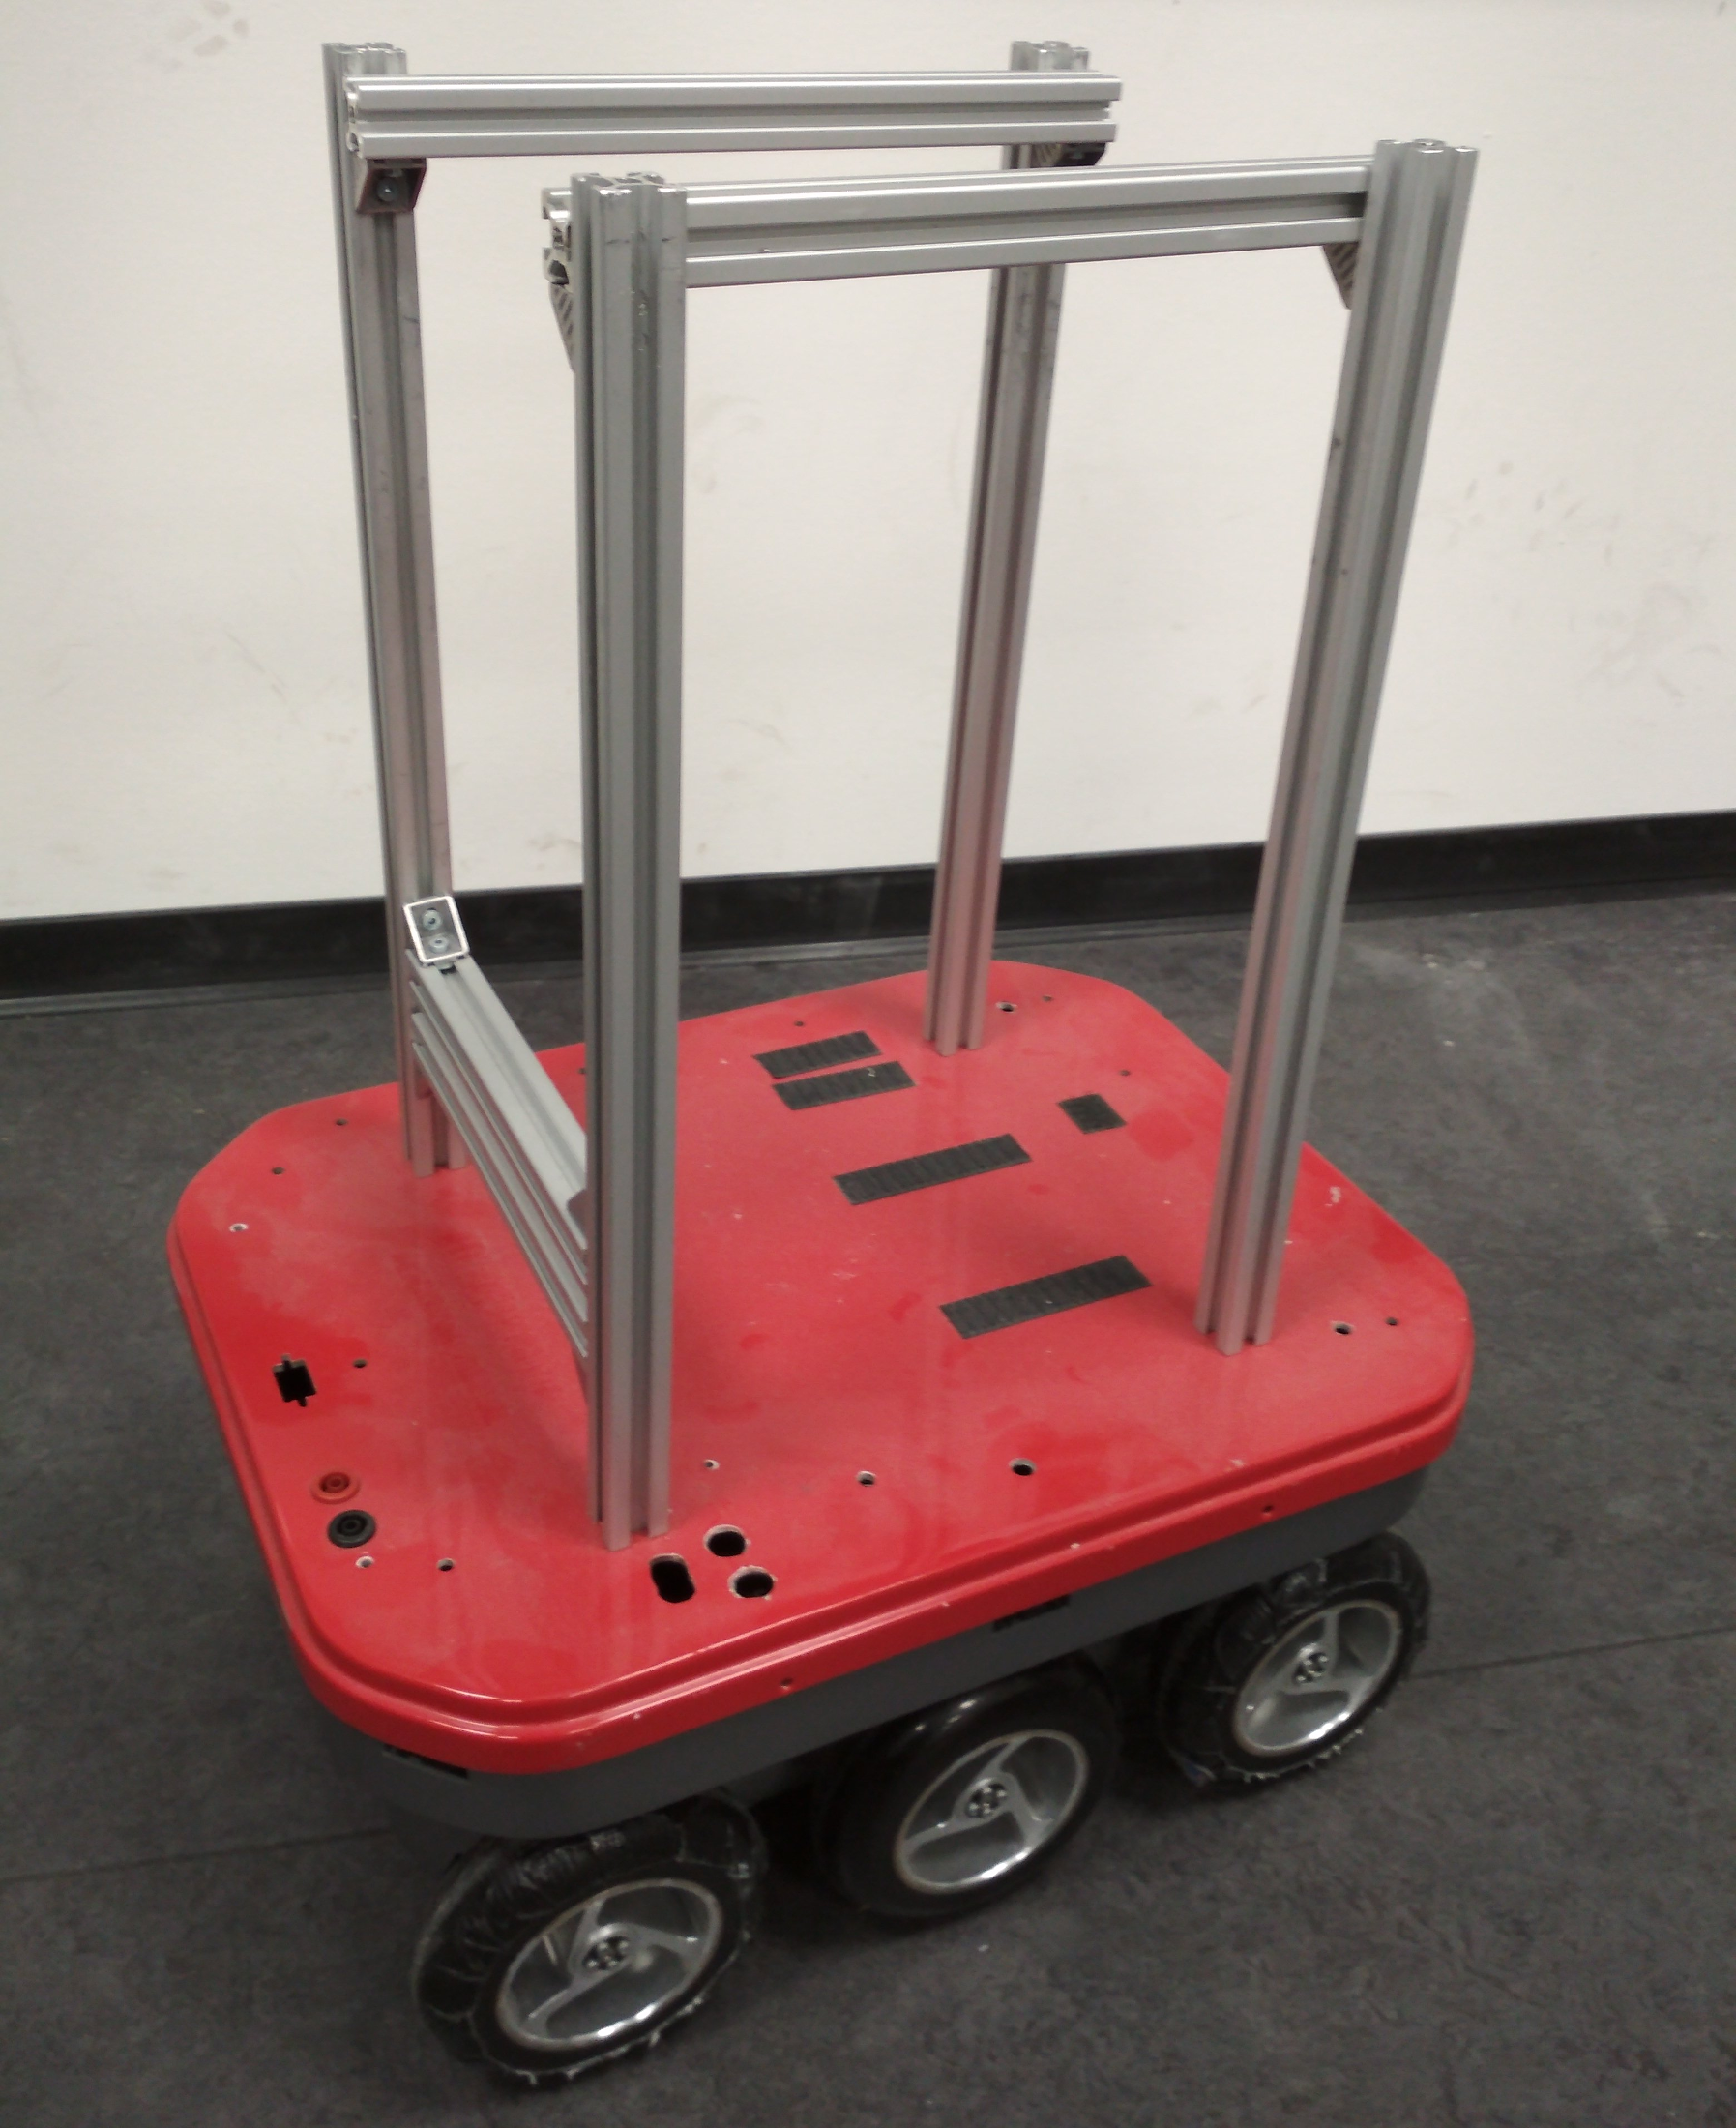
\includegraphics[width=0.35\textwidth]{KURT.png}
    \caption{Der KURT2-Roboter, dessen Hardware ersetzt werden soll.}
    \label{fig:kurt}
\end{wrapfigure}

KURT2 ist eine universelle Roboterplattform die 2003 vom Fraunhofer AiS
(Institut für Autonome intelligente Systeme) vorgestellt wurde und seitdem den
Weg an einige Universitäten gefunden hat \cite{kurt2-zdnet}. KURT2 ging aus KURT
hervor, der
\textbf{K}anal\-\textbf{u}ntersuchungs\hyp{}\textbf{R}oboter\textbf{t}estplattform
\cite{kurt2-home}.

Ein KURT2-Roboter ist ausgestattet mit einem Akku, 2 Gleichstrommotoren samt
Encodern zur Positionsbestimmung, Sonarsensoren und Bumper zur
Hinderniserkennung und einem elektronischen Kompass. Die Gleichstrommotoren
bilden einen Differentialantrieb, bei dem jeder Motor die Räder auf einer Seite
des Roboters antreibt. Die Elektronik besteht aus einem 16-bit Mikrocontroller
von Infineon und wird per CAN-Bus entweder an einen externen Laptop oder einen
PC/104 embedded PC angebunden \cite{kurt2-hardware}.

Da moderne Computer im Allgemeinen nicht mit einem CAN-Port ausgestattet sind,
wird hierzu ein Adapter benötigt, was die Nutzung verkompliziert.


\section{Raspberry Pi}

\begin{wrapfigure}[12]{r}{0.45\textwidth}
    \vspace{-8pt}
    \centering 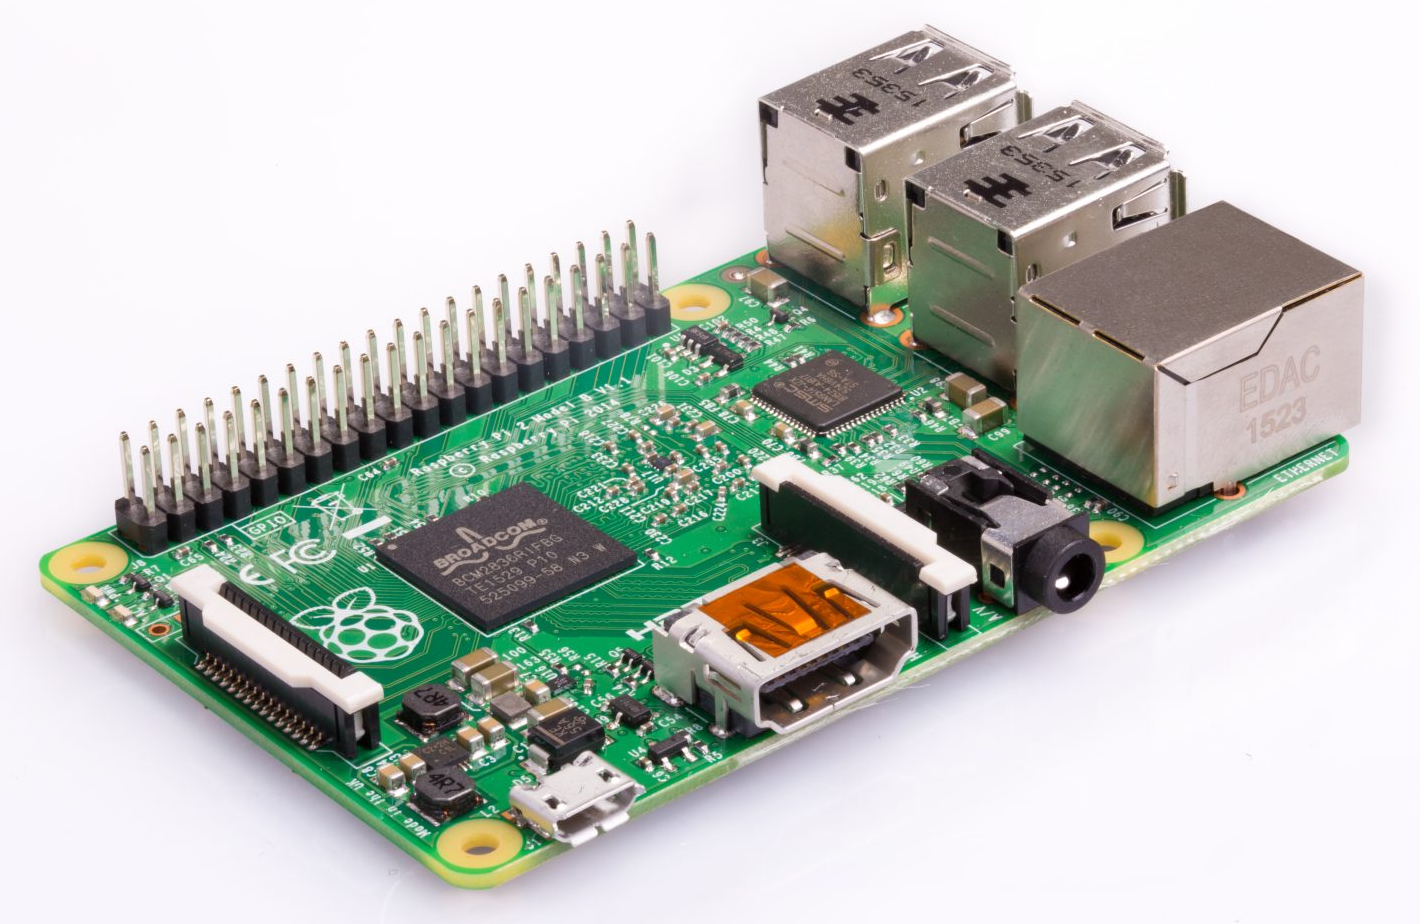
\includegraphics[width=0.45\textwidth]{Pi.png}
    \caption{Raspberry Pi 2 Model B. Bildquelle: \cite{raspi2b}.}
    \label{fig:raspi}
\end{wrapfigure}

Raspberry Pi ist eine Reihe günstiger, kreditkartengroßer Einplatinencomputer,
die von der Raspberry Pi Foundation entwickelt und vertrieben wird
\cite{raspi-web}.

Das erste Modell wurde im Jahr 2012 auf den Markt gebracht \cite{raspi-launch}.
Seitdem wurden zahlreiche verbesserte Modelle sowie Zubehör und Add-On Boards
entwickelt und es hat sich eine große Community gebildet. Nicht zuletzt dank
dieser ist eine große Auswahl an Software für Raspberry Pis verfügbar.

Da die Raspberry Pi Foundation mit dem Ziel gegründet wurde, die Bildung im
IT-Bereich zu verbessern, existieren sehr gute Ressourcen um mit der Plattform
vertraut zu werden \cite{raspi-strategy} \cite{raspi-docs}. Hard- und Software,
die von der Raspberry Pi Foundation veröffentlicht wurde, ist meistens exzellent
dokumentiert.

Für diese Arbeit wurde ein Raspberry Pi 2 Model B genutzt. Die
Software sollte ohne Änderungen auf allen Raspberry Pi 2 und 3 Varianten
funktionieren.

Der Raspberry Pi 2B besitzt eine 4-Kern ARM Cortex-A7 CPU, die mit 900 MHz
getaktet ist \cite{raspi2b}. Da die Hardware der KURT2-Roboter mittlerweile ca.
15 Jahre alt ist, sollte dies ein beachtliches Upgrade in Bezug auf
Rechenleistung darstellen. Für weniger rechenintensive Aufgaben kann der
Raspberry Pi auch ohne externen Computer genutzt werden. Die CPUs sind, wie bei
allen bisher vermarkteten Raspberry Pi Modellen, Teil eines Broadcom SoCs
(System-on-a-chip), der unter anderem eine OpenGL-fähige VideoCore IV GPU und
einige Hardwarebausteine zur Anbindung externer Komponenten bereitstellt.

Die meisten Raspberry Pi Modelle verfügen über einen Erweiterungssteckplatz, auf
dem einige GPIOs (General Purpose Inputs/Outputs) untergebracht sind, die sich
für beliebige Anwendungen einsetzen lassen und per Software steuerbar sind.

Jeder Raspberry Pi des B-Modells verfügt außerdem über einen LAN-Port, der hier
anstelle des CAN-Buses zur Kommunikation mit einem externen Computer genutzt
werden soll. Um dies möglichst einfach zu gestalten, ist der Raspberry Pi mit
der festen IP \code{192.168.100.1} konfiguriert (sowie einer Subnetzmaske von
\code{255.255.255.0}, sodass jedes Gerät im \code{192.168.100.*}-Netz erreichbar
ist). Zusätzlich ist auch mDNS eingerichtet, ein serverloses Protokoll zur
Namensauflösung, womit der Raspberry Pi unter \code{kurtberry-pi.local}
erreichbar ist.

Als Basis für die Software wurde ein auf Ubuntu basierendes SD-Karten-Image von
German-Robot.com verwendet, welches für die Verwendung für Robotern
zugeschnitten ist und viele benötigte Pakete bereits enthält, wodurch die
Installation vereinfacht wird \cite{pi-image}.

Da Ubuntu die ARMv6 Architektur nicht unterstützt, die von den älteren Raspberry
Pi Modellen verwendet wird, muss für diese Modelle eine andere Distribution wie
Raspbian oder Arch Linux ARM verwendet werden \cite{ubuntu-arm-support}
\cite{raspbian-arm-support} \cite{alarm-armv6-support}.


\section{Motivation und Zielsetzung}

Die Hardware der KURT2-Roboter ist mittlerweile fast vollständig veraltet. Indem
sie durch einen Raspberry Pi ersetzt und massiv vereinfacht wird, wird der
modifizierte Roboter zugänglicher für Studenten und wird zu einer leicht nutz-
und modifizierbaren Basisplattform.

Allerdings soll die Hardware nicht vollständig ersetzt werden: Der Akku, die
Motoren sowie die Motortreiber sind noch voll funktionsfähig und sollen
beibehalten werden. Außerdem wird ein auf der alten Hauptplatine verlöteter
Spannungswandler wiederverwendet, um die Versorgungsspannung des Raspberry Pis
aus der Batteriespannung abzuleiten. Dies wird genauer in \autoref{ch:hardware}
erläutert.

Die Anbindung der Sonarsensoren und Bumper ist nicht Teil dieser Arbeit. Während
sich diese Sensoren zwar zur Hinderniserkennung eignen, können sie durch einen
externen Laserscanner ersetzt werden, der weitaus höher aufgelöste Daten
liefert, die sich auch zur Lokalisierung und zum Kartieren der Umgebung eignen,
womit die Funktion der Sonarsensoren größtenteils redundant erscheint.

Der auf dem alten KURT2-Mainboard vorhandene elektronische Kompass geht durch
den Umbau verloren, kann aber bei Bedarf durch eine USB-IMU ersetzt werden, die
am Raspberry Pi angeschlossen wird. Eine IMU (Inertial Measurement Unit) misst
Winkel- und Linearbeschleunigung (6 Freiheitsgrade) und je nach Modell auch die
Magnetfeldstärke in 3 Dimensionen.

Die Rechenleistung des Raspberry Pi ist ausreichend für simple Aufgaben, weshalb
nicht immer ein externer Computer angeschlossen werden muss. Wenn dies nötig
ist, ist die Anbindung einfacher als bei der originalen Hardware, da kein
CAN-Bus genutzt wird und somit kein Adapter nötig ist. Stattdessen wird der
LAN-Port des Raspberry Pis genutzt.


\chapter{Hardware}
\label{ch:hardware}

Die Motoren und Motortreiber sowie der NiMH-Akku des KURT2-Roboters wurden
wiederverwendet, während die Steuerungselektronik ausgetauscht wurde.
Insbesondere die Wiederverwendung der Treiber vereinfacht den Designprozess, da
sichergestellt ist, dass die gesamte Leistungselektronik den Anforderungen
gerecht wird.

Zusätzlich wurde auch ein auf dem alten Mainboard verbauter 5V-Spannungsregler
wiederverwendet, um von der Batteriespannung von etwa 36V die Betriebsspannung
für den Raspberry Pi abzuleiten.

Anders als bei der Originalhardware wird kein Mikrocontroller benötigt. Die
gesamte Datenverarbeitung läuft auf dem Raspberry Pi ab. Das bedeutet, dass nur
ein einzelnes Softwarepaket erforderlich ist und keine Compilertoolchain zum
Kompilieren von Mikrocontrollercode benötigt wird.


\section{Motortreiber}
\label{section:Motortreiber}

\begin{wrapfigure}[12]{r}{0.4\textwidth}
    \vspace{-11pt}
    \centering \includegraphics[width=0.4\textwidth]{h-bridge-photo-cropped.png}
    \caption{Einer der beiden Motortreiber des Roboters.}
    \label{fig:motor-module}
\end{wrapfigure}

Die genaue Funktionsweise der Treibermodule war zunächst nicht bekannt, da kein
Schaltplan vorlag. Um damit arbeiten zu können war also notwendig, im Nachhinein
einen vereinfachten Schaltplan der Module anzufertigen. Dieser wird in
\autoref{fig:motor-module} gezeigt.

\begin{figure}[!ht]
    \centering 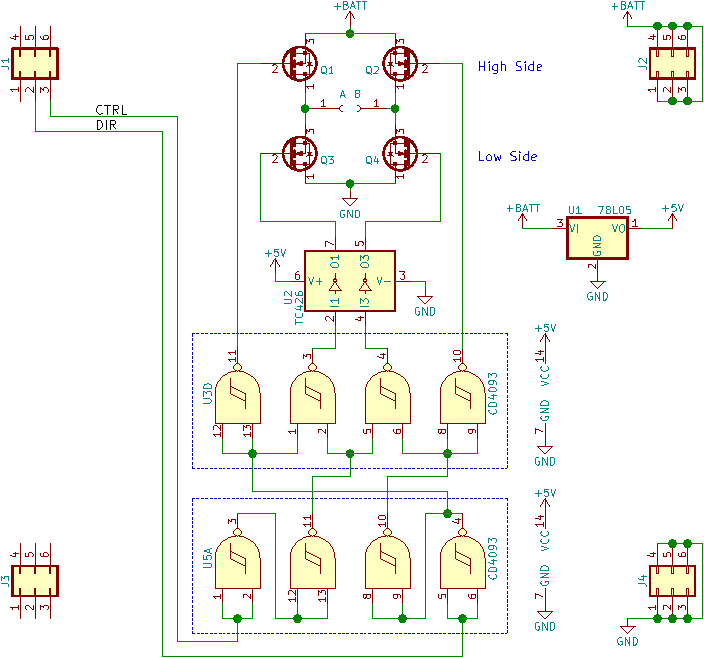
\includegraphics[width=15cm]{kicad/motor-module/motor-module-cropped.pdf}
    \caption{Vereinfachter Schaltplan eines Motortreibers. Die Positionen der
        Steckverbinder (\code{J1, J2, J3, J4}) stimmen mit denen auf der Platine
        überein (Draufsicht). Die High-Side MOSFETs verfügen über integrierte
        Treiber, weshalb nur ein TC426 für die Low-Side MOSFETs eingezeichnet
        ist.}
    \label{fig:motor-module}
\end{figure}

Die Treibermodule werden über zwei Steuersignale kontrolliert. Ein Signal
bestimmt, ob eine Spannung am Motor anliegt (\code{CTRL}), das andere bestimmt
die Polarität und somit die Drehrichtung des Motors (\code{DIR}).

Beide Module sind identisch aufgebaut. Jedes besteht aus einer H-Brücke und
diskreter Logik, die die Steuersignale in Schaltzustände der Transistoren
umsetzt.

% \begin{wrapfigure}{r}{0.45\textwidth}
%     \centering 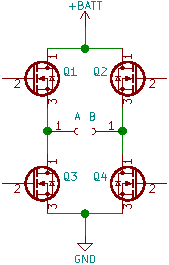
\includegraphics[width=4cm]{kicad/h-bridge/h-bridge-cropped.pdf}
%     \caption{Schaltplan einer H-Brücke.}
%     \label{fig:h-bridge}
% \end{wrapfigure}

Eine H-Brücke ist eine Anordnung von 4 Transistoren, die eine Last (in diesem
Fall den Motor) mit wählbarer Polarität mit der Versorgungsspannung verbinden
kann, abhängig von den Schaltzuständen der Transistoren. Im Schaltplan in
\autoref{fig:motor-module} wird die H-Brücke durch die Transistoren
\code{Q1}, \code{Q2}, \code{Q3} und \code{Q4} gebildet, die Teil eines BTS7810K
ICs sind \cite{h-bridge-datasheet}. Der Motor wird an den Punkten \code{A} und
\code{B} angeschlossen.

Das genaue Verhalten der H-Brücke und des angeschlossenen Motors für die
möglichen Transistorzustände ist in \autoref{tbl:h-bridge} beschrieben. Das
gleichzeitige Leiten von \code{Q1} und \code{Q3} bzw. von \code{Q2} und
\code{Q4} schließt die Batterie kurz, da dann \code{+BATT} mit \code{GND}
verbunden ist. Um diese Kurzschlusszustände zu vermeiden, werden auf den Modulen
verbaute diskrete Logikgatter eingesetzt. Bei moderneren Treiberbausteinen wie
dem L298 sind ähnliche Logikschaltungen bereits integriert, wodurch die Anzahl der notwendigen ICs minimiert wird \cite{l298-datasheet}.

\begin{table}%{l}{0.5\textwidth}
    \centering
    \begin{tabular}{|l|l|l|l|l|}
        Q1  & Q2  & Q3  & Q4  & Verhalten \\ \hline
        0   & 0   & 0   & 0   & Kein Stromfluss \\
        0   & 0   & 0   & 1   & Kein Stromfluss \\
        0   & 0   & 1   & 0   & Kein Stromfluss \\
        0   & 0   & 1   & 1   & Motor bremst \\
        0   & 1   & 0   & 0   & Kein Stromfluss \\
        0   & 1   & 0   & 1   & Kurzschluss \\
        0   & 1   & 1   & 0   & B an +, A an - \\
        0   & 1   & 1   & 1   & Kurzschluss \\
        1   & 0   & 0   & 0   & Kein Stromfluss \\
        1   & 0   & 0   & 1   & A an +, B an - \\
        1   & 0   & 1   & 0   & Kurzschluss \\
        1   & 0   & 1   & 1   & Kurzschluss \\
        1   & 1   & 0   & 0   & Motor bremst \\
        1   & 1   & 0   & 1   & Kurzschluss \\
        1   & 1   & 1   & 0   & Kurzschluss \\
        1   & 1   & 1   & 1   & Kurzschluss \\
    \end{tabular}
    \caption{
        Die 16 Transistorzustände einer H-Brücke und das resultierende
        Verhalten. Die Kurzschlusszustände gilt es zu vermeiden.
    }
    \label{tbl:h-bridge}
\end{table}

Bei den verwendeten Logikgattern handelt es sich um CD4093 Quad-NAND-Bausteine
\cite{nand-datasheet}. Die Schaltzustände der vier Transistoren in der H-Brücke
werden durch die Zustände der \code{CTRL} und \code{DIR} Steuersignale anhand
folgender Formeln bestimmt, die aus dem erstellten Schaltplan in
\autoref{fig:motor-module} abgeleitet wurden:

\begin{align}
    Q1 &= \neg \neg \mathit{DIR} = \mathit{DIR} \\
    Q2 &= \neg \neg \neg \mathit{DIR} = \neg \mathit{DIR} \\
\begin{split}
    Q3 &= \neg ((\neg \mathit{DIR}) \mathit{NAND} (\neg \neg \mathit{CTRL})) \\
       &= \neg \neg ((\neg \mathit{DIR}) \wedge (\neg \neg \mathit{CTRL})) \\
       &= \mathit{CTRL} \wedge \neg \mathit{DIR}
\end{split} \\
\begin{split}
    Q4 &= \neg ((\neg \neg \mathit{CTRL}) \mathit{NAND} (\neg \neg \mathit{DIR})) \\
       &= \neg \neg ((\neg \neg \mathit{CTRL}) \wedge (\neg \neg \mathit{DIR})) \\
       &= \mathit{CTRL} \wedge \mathit{DIR}
\end{split}
\end{align}

Die Zustände von \code{Q3} und \code{Q4} werden zusätzlich durch den
MOSFET-Treiber TC426 invertiert. Diese Negation ist in den obigen Formeln
bereits enthalten.

Die aus den 4 Kombinationen aus \code{CTRL} und \code{DIR} resultierenden
Transistorzustände sind in \autoref{tbl:ctrl-dir-states} aufgeführt.

\begin{table}
    \centering
    \begin{tabular}{|l|l|l|l|l|l|l|}
        CTRL & DIR & Q1  & Q2  & Q3  & Q4  & Verhalten       \\ \hline
        0    & 0    & 0   & 1   & 0   & 0   & Kein Stromfluss \\
        0    & 1    & 1   & 0   & 0   & 0   & Kein Stromfluss \\
        1    & 0    & 0   & 1   & 1   & 0   & B an +, A an -  \\
        1    & 1    & 1   & 0   & 0   & 1   & A an +, B an -  \\
    \end{tabular}
    \caption{
        Motorverhalten und Transistorzustände in Abhängigkeit von den
        Zuständen der \code{CTRL} und \code{DIR} Steuersignale. Die in
        \autoref{tbl:h-bridge} aufgelisteten Kurzschlusszustände können nicht
        auftreten.
    }
    \label{tbl:ctrl-dir-states}
\end{table}

Beim Umschalten des Richtungssignals \code{DIR} müssen die aktiven Transistoren
auf einer Seite der H-Brücke gewechselt werden (vgl. die letzten 2 Zeilen von
\autoref{tbl:ctrl-dir-states}). Dabei schalten nie beide Transistoren zum exakt
gleichen Zeitpunkt an bzw. aus, weshalb für kurze Zeit beide leiten können und
effektiv einen temporären Kurzschluss erzeugen. Wird \code{DIR} mit hoher
Frequenz geschaltet (einige hundert Hertz), gibt die H-Brücke ein Geräusch von
entsprechender Frequenz von sich und erwärmt sich merklich.

Dies kann verhindert werden, indem mit einer Totzeit sichergestellt wird, dass
beim Umschalten für kurze Zeit keiner der beiden Transistoren auf einer Seite
leitet. Die Motortreiber verfügen allerdings über keine Hardware dafür. Aus
diesem Grund soll durch die Software die Anzahl der Richtungsänderungen pro
Sekunde limitiert werden, wodurch dieser Effekt auf ein Minimum begrenzt wird.

Da die Treibermodule einen Logikpegel von 5V verwenden, Raspberry Pis aber
3,3V-Logik einsetzen, müssen die Signale umgewandelt werden. Dazu wird ein
sogenannter Level-Shifter vom Typ SN74HC245 verwendet
\cite{levelshifter-datasheet}.


\section{Encoder}

Um einen geschlossenen Regelkreis zu erhalten, muss die aktuelle
Motorgeschwindigkeit vom Raspberry Pi erfasst werden. Dieses Feedback erlaubt
dann dem Regler eine vorgegebene Radgeschwindigkeit anzusteuern und zu halten,
unabhängig vom Gewicht des Roboters oder der Batterieladung.

\begin{figure}[h]
    \centering
    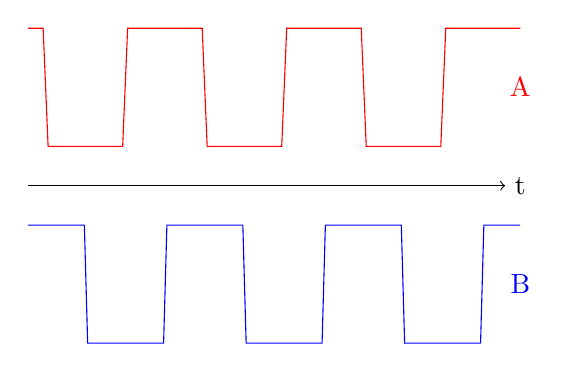
\begin{tikzpicture}
        \draw[domain=0.75:7,variable=\x,samples=100,color=red]
            plot ({\x},{(Mod(\x*0.5, 1) < 0.5) * 1.5 + 2.5});

        \draw[domain=0.75:7,variable=\x,samples=150,color=blue]
            plot ({\x},{(Mod(\x*0.5-0.25, 1) < 0.5) * 1.5});

        \node (t) at (7,2) {t};
        \draw[->] (0.75,2) -- (t);

        \node[color=red] (a) at (7,3.25) {A};
        \node[color=blue] (b) at (7,0.75) {B};
    \end{tikzpicture}
    \caption{
        Verlauf eines Encodersignals bei Vorwärtsdrehung.
    }
    \label{fig:encoder-signal}
\end{figure}

Zum Auslesen der Geschwindigkeit werden sogenannte Drehgeber oder Encoder
verwendet. Diese verwenden meist eine mit der Achse mitdrehende Plastikscheibe,
an deren Rand sich Löcher befinden. Durch einen am stationären Teil des Encoders
befindlichen optischen Detektor können so die Löcher erkannt werden und ein
elektrisches Signal erzeugt werden. Je schneller sich die Achse dreht, desto
höher die Frequenz des ausgegebenen Signals. Um zusätzlich zur
Winkelgeschwindigkeit auch die Drehrichtung bestimmen zu können, sind zwei
Photodetektoren verbaut, die um 90$^\circ$ phasenverschoben zueinander messen
und ihre Ausgangssignale an 2 Kanälen A und B zur Verfügung stellen. Der
resultierende Signalverlauf wird in \autoref{fig:encoder-signal} verdeutlicht.

Verfolgt man das Signal des A-Kanals, so fällt auf, dass bei jeder steigenden
Flanke auf dem A-Kanal der Pegel auf dem B-Kanal niedrig (logisch 0) ist. Läuft
man das Signal hingegen von der anderen Richtung ab (von rechts nach links), was
einer Rückwärtsdrehung des Encoders entspricht, so ist das B-Signal bei jeder
steigenden Flanke im A-Kanal auf \emph{hohem} Pegel (logisch 1). Auf diese Weise
kann die Drehrichtung per Software erkannt werden, während die Signale gezählt
werden.

Die Anbindung der Encoder gestaltet sich relativ einfach: Sie benötigen
keinerlei externe Hardware und können mit 3,3 V versorgt werden, wodurch kein
Level-Shifter notwendig ist. Da der Raspberry Pi über einen integrierten
Spannungsregler eine Spannung von 3,3 V aus der Versorgungsspannung ableitet,
kann diese direkt für die Encoder genutzt werden.

% TODO: Encodertyp erwähnen!


\section{Basisplatine}

\begin{figure}
    \centering
    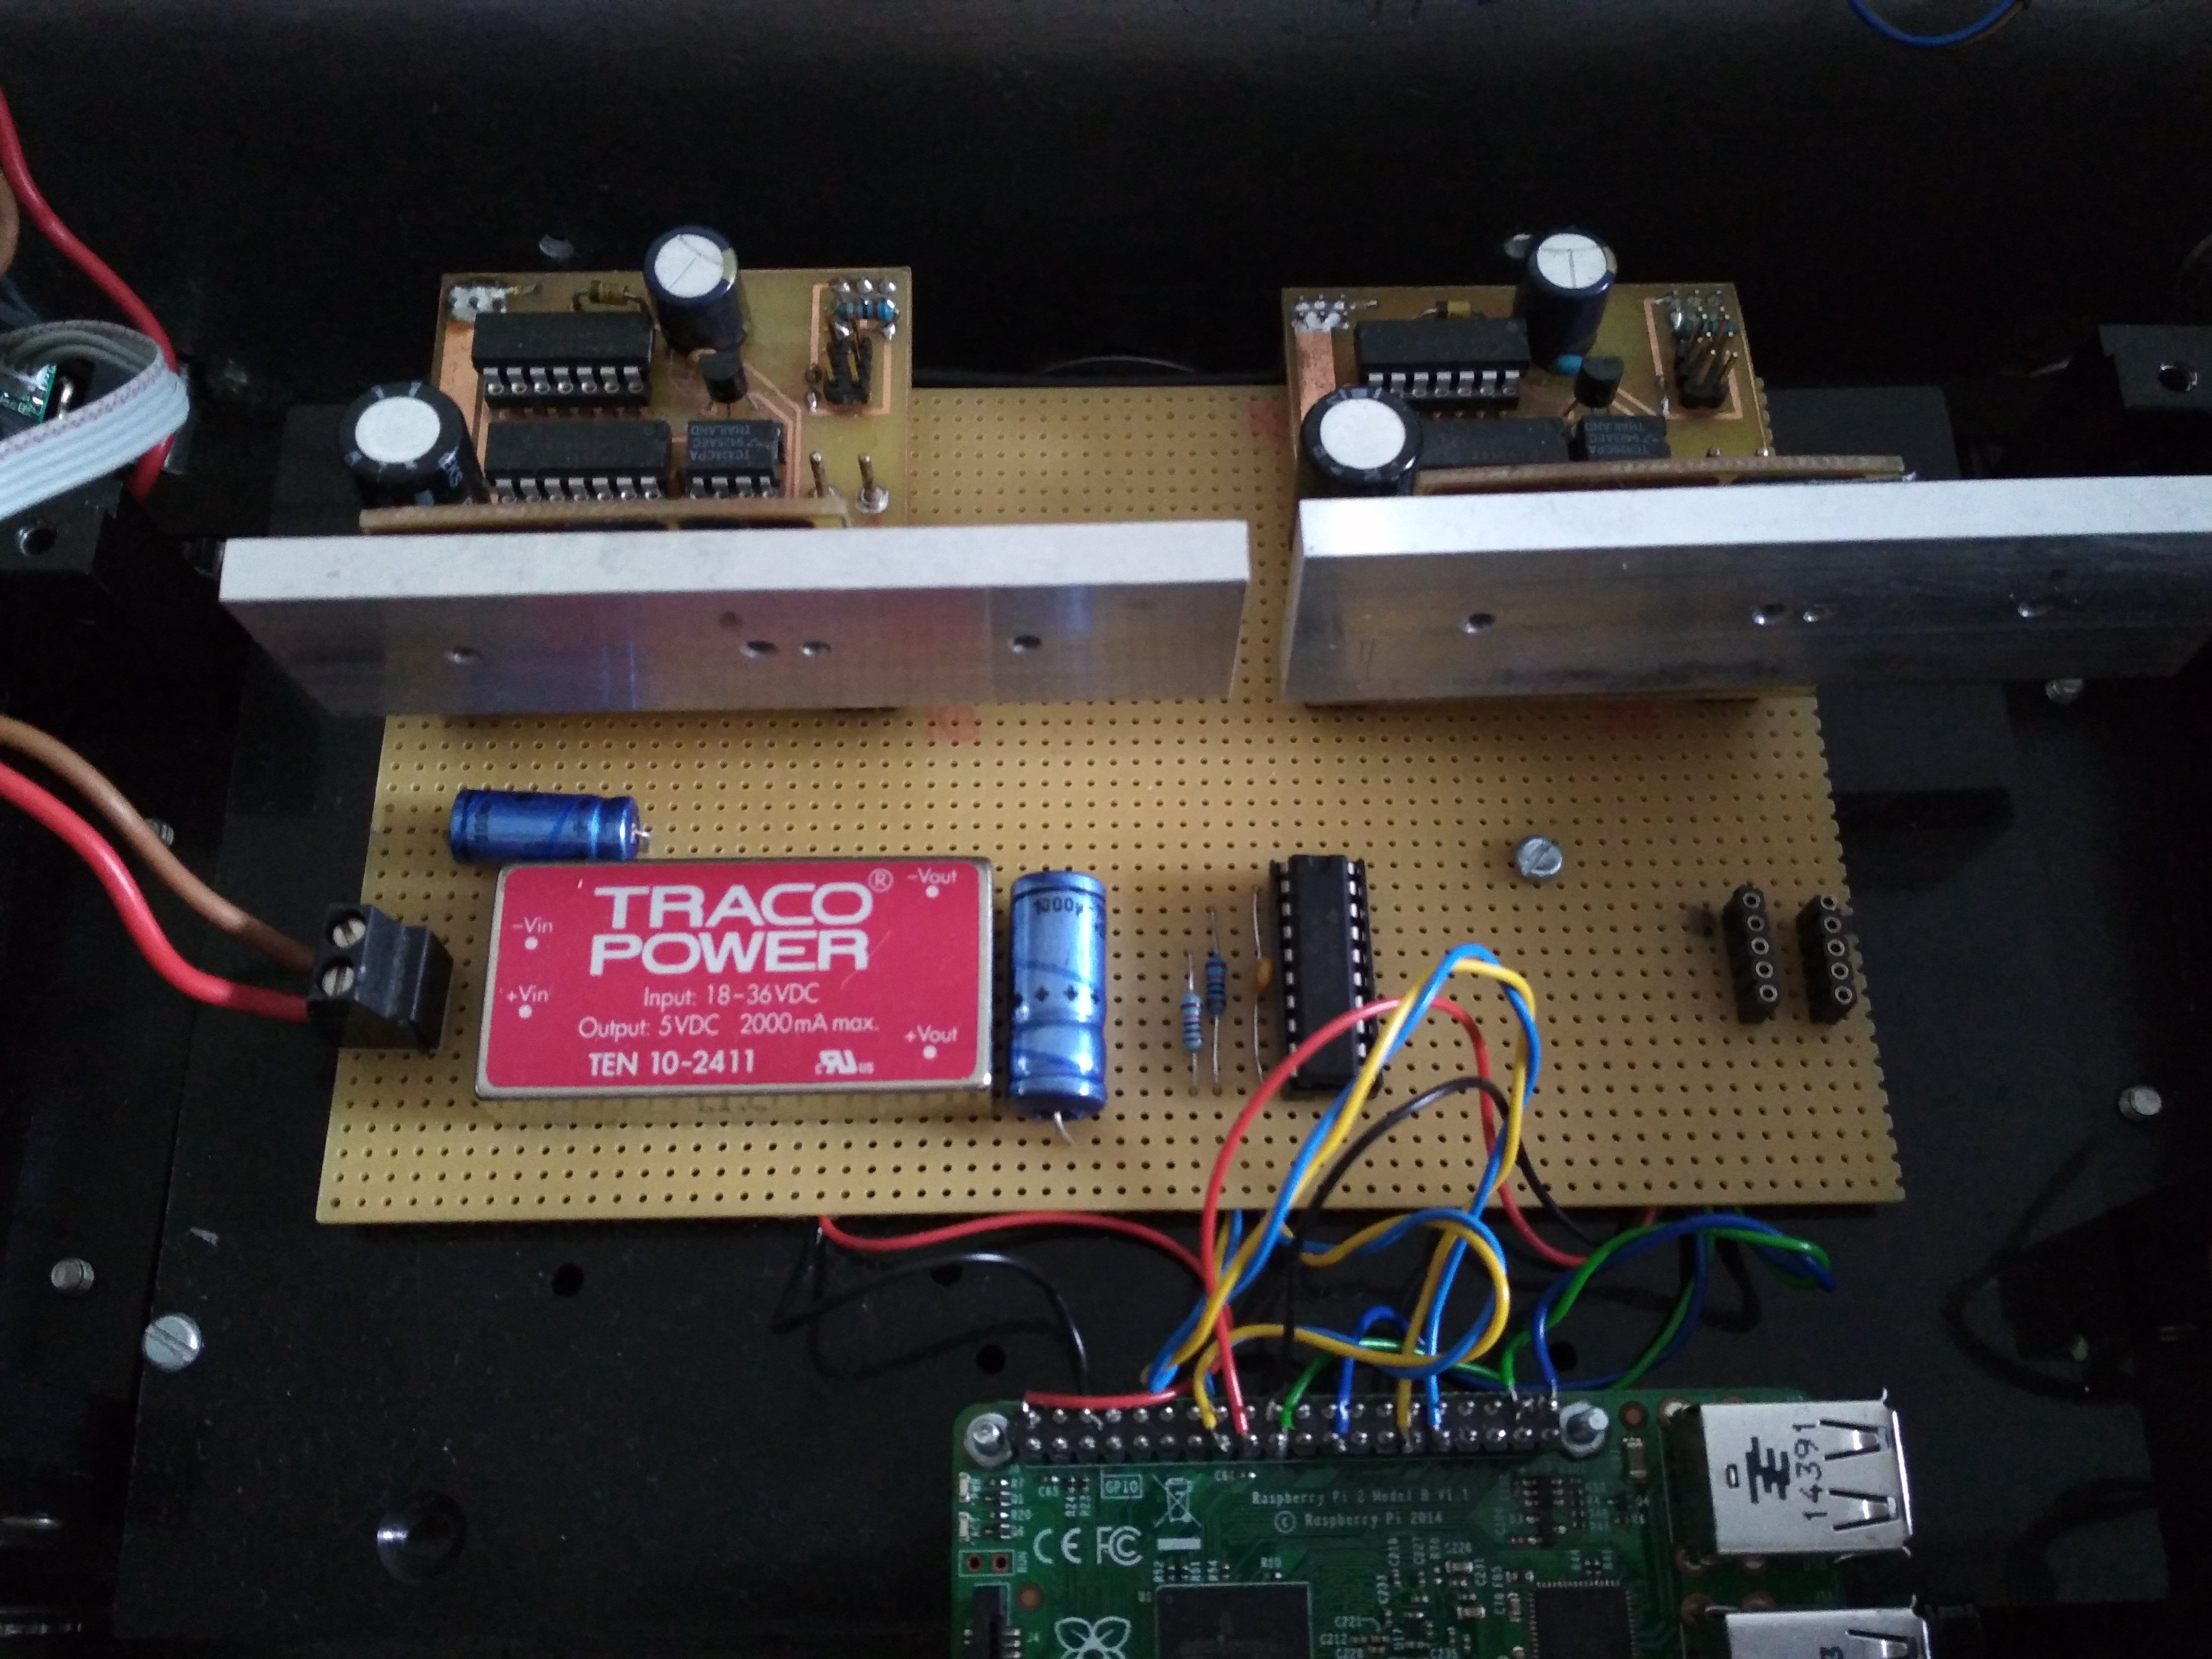
\includegraphics[width=0.9\textwidth]{electronics.jpg}
    \caption{
        Basisplatine mit montierten Motortreibern.
    }
    \label{fig:basisplatine}
\end{figure}

\begin{figure}
    \centering
    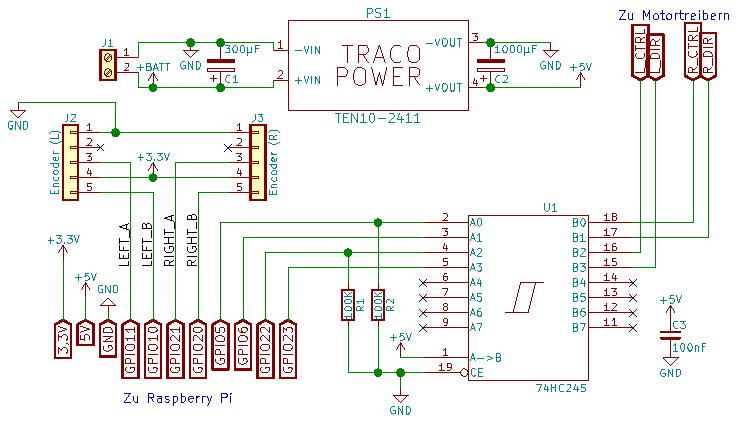
\includegraphics[width=\textwidth]{kicad/electronics/electronics-cropped.pdf}
    \caption{
        Vereinfachter Schaltplan von Spannungsregler und Level Shifter.
    }
    \label{fig:electronics-schematic}
\end{figure}

Um die Elektronik im Gehäuse des KURT2-Roboters unterzubringen, wurden
Motortreiber und restliche Elektronik auf einer Lochrasterplatine montiert, die
in \autoref{fig:basisplatine} zu sehen ist. Die Motortreiber werden in
Buchsenleiten gesteckt, die auf der Hauptplatine verlötet sind, wodurch sich die
Treiber sehr einfach entfernen und austauschen lassen. Die Verbindungen zum
Raspberry Pi werden ebenfalls über eine Buchsenleiste geführt, die auf die
Stiftleiste gesteckt wird. Somit lässt sich auch der Raspberry Pi durch ein
pinkompatibles Modell austauschen.

\autoref{fig:electronics-schematic} zeigt einen groben Schaltplan der auf der
Basisplatine vorhandenen Komponenten, der einen Überblick über die elektrischen
Verbindungen geben soll.

Am Batterieanschluss sowie nach dem Spannungsregler wurden
Elektrolytkondensatoren zum Puffern der Versorgungsspannung verlötet, um
Spannungseinbrüche beim Schalten der Motoren zu mindern. Der 100 nF
Keramikkondensator am Level Shifter ist ein Entkopplungskondensator, der bei
Schaltvorgängen die möglicherweise entstehenden Stromspitzen bereitstellt.

Die \code{CTRL}-Leitungen werden durch 2 Pull-Down-Widerstände an den Eingängen
des Level Shifters auf Masse gezogen, wodurch die Motortreiber standardmäßig
abgeschaltet sind, wenn der Raspberry Pi sie nicht aktiv einschaltet. Fehlen
diese Widerstände, würden die Motoren beispielsweise beim Neustart des Raspberry
Pis unkontrolliert einschalten, was vermieden werden muss.

Zwei Kontakte des Spannungswandlers, \code{-VIN} und \code{-VOUT}, wurden
miteinander verbunden. Da es sich um einen isolierenden Wandler handelt, der
eine Ausgangsspannung erzeugt, die vollständig galvanisch getrennt von der
Eingangsspannung ist, ist diese Verbindung notwendig, um zwischen beiden Seiten
Signale austauschen zu können. Die Verbindung stellt die gemeinsame Masse wieder
her und erlaubt das Schalten der Motortreiber (die am \code{-VIN}-Netz
angeschlossen sind) durch den Raspberry Pi und Level Shifter (die beide am
\code{-VOUT}-Netz angeschlossen sind).

\autoref{tbl:pi-pins} stellt eine Zuordnung aller verwendeten Pins der
Stiftleiste auf dem Raspberry Pi dar und kann genutzt werden, um die von einem
GPIO-Pin erfüllte Funktion einzusehen (oder umgekehrt, den einer Funktion
zugeordneten GPIO-Pin).

\begin{table}
    \centering
    \begin{tabular}{|l|l|l|l|}
        Pin-Name & Pin\# & Funktion                  & Farbe      \\ \hline
        5V       & 2     & Pi-Versorgungsspannung    & Rot        \\
        GND      & 6     & Gemeinsame Erdung         & Schwarz    \\
        3.3V     & 17    & 3,3V Spannung für Encoder & Rot        \\
        GND      & 20    & Erdung für Encoder        & Schwarz    \\
        GPIO22   & 15    & \code{CTRL} linker Motor  & Gelb       \\
        GPIO23   & 16    & \code{DIR} linker Motor   & Hellblau   \\
        GPIO5    & 29    & \code{CTRL} rechter Motor & Gelb       \\
        GPIO6    & 31    & \code{DIR} rechter Motor  & Hellblau   \\
        GPIO21   & 40    & Kanal A linker Encoder    & Dunkelblau \\
        GPIO20   & 38    & Kanal B linker Encoder    & Grün       \\
        GPIO11   & 23    & Kanal A rechter Encoder   & Dunkelblau \\
        GPIO10   & 19    & Kanal B rechter Encoder   & Grün       \\
    \end{tabular}
    \caption{
        Belegung der GPIO-Pins des Raspberry Pis. Pin\# bezeichnet die Nummer
        des Pins auf der Stiftleiste, während der Pin-Name der vom Raspberry Pi
        genutzte Bezeichner für den Pin ist. Zur Pinbelegung des Raspberry Pis
        siehe \cite{pi-gpio-pinout}.
    }
    \label{tbl:pi-pins}
\end{table}

% level shifter verbindung:
%   => oben = Treiber links, rechter Motor; darunter = Treiber rechts, linker Motor

Die Basisplatine und der Raspberry Pi sind auf einer nichtleitenden
Plastikplatte verschraubt, die wiederum in die im Roboterchassis vorhandenen
Gewinde geschraubt ist.



\chapter{Software}

Die Software, die im Rahmen dieser Arbeit geschrieben wurde, ist auf dem
Uni-internen GitLab-Server unter
\url{https://gitlab.informatik.uni-osnabrueck.de/jschievink/kurtberry-pi}
abgelegt. Alle Pfadangaben im folgenden Teil sind, sofern nicht anders
angegeben, relativ zu diesem Repository.

Der hier beschriebene Softwarestack läuft auf dem Raspberry Pi und übernimmt die
Regelung der Motorgeschwindigkeit sowie die Anbindung der Hardware an das Robot
Operating System (ROS) \cite{ros-web}. ROS ist ein etabliertes Robotikframework
und wird seit langem von der Universität für viele Robotikprojekte eingesetzt.

Um ROS einzusetzen, muss zuerst ein ROS-Core gestartet werden, der eine zentrale
Datenbank aller Bestandteile des ROS-Systems führt, mithilfe dieser
eigenständige ROS-Programme (sogenannte ROS-Nodes) miteinander kommunizieren
können. Im Rahmen dieser Arbeit wurde der ROS-Node \code{kurtberry\_pi\_node}
geschrieben, der Teil des \code{kurtberry\_pi}-Pakets ist und mithilfe bereits
bestehender ROS-Nodes die Steuerung des Roboters durchführt.

Da übliche ROS-Systeme viele Nodes enthalten, lässt sich das Starten dieser über
Launch-Files vereinfachen. Mit dem \code{roslaunch}-Befehl lässt sich eine
\code{.launch}-Datei starten, die Nodes definieren und Parameter festlegen kann.
In \path{launch/kurt.launch} findet sich das Launch-File das zum Starten der
benötigten KURT2-Nodes genutzt werden kann.

ROS bietet flexible Möglichkeiten für Interprozesskommunikation (IPC), die es
ermöglichen, Teile einer Robotikanwendung auf verschiedene Computer im Netzwerk
auszulagern, ohne dass deren Funktion oder Kommunikation eingeschränkt wird.

Dies kann beispielsweise genutzt werden, um den Raspberry Pi via Ethernet mit
einem leistungsfähigeren Computer zu verbinden. Dazu wird ein einziger
\code{roscore} genutzt, der auf einem der beiden Computer läuft. Auf dem anderen
Computer kann dann allen ROS-Nodes mitgeteilt werden, dass der \code{roscore}
auf einem anderen System läuft, indem die Umgebungsvariable
\code{ROS\_MASTER\_URI} wie folgt gesetzt wird \cite{roscore}:

\begin{lstlisting}[numbers=none]
    export ROS_MASTER_URI=http://CORE_COMPUTER:PORT/
\end{lstlisting}

Dabei ist \code{CORE\_COMPUTER} der Hostname oder die IP-Adresse des Computers,
auf dem der \code{roscore} läuft, und \code{PORT} der Port den der Core für
Netzwerkanfragen nutzt. Standardmäßig wird beim Start eines \code{roscore} ein
zufälliger Port gewählt. Indem der \code{-p} Parameter beim Start des Cores
angegeben wird, kann ein fester Port definiert werden:

\begin{lstlisting}[numbers=none]
    roscore -p 1234
\end{lstlisting}

Die Kommunikation zwischen ROS-Nodes findet üblicherweise nach dem
Publish-Subscribe Prinzip statt. Es können Topics definiert werden, auf denen
Nachrichten eines festen Typs veröffentlicht werden können. Interessierte
ROS-Nodes können sich dann als \emph{Subscriber} eintragen und bekommen alle
Nachrichten, die dort veröffentlicht werden, zugestellt
\cite{rostopic-tutorial}.

Das Kommandozeilentool \code{rostopic} kann verwendet werden, um verfügbare
Topics aufzulisten und die darauf veröffentlichten Nachrichten mitzuverfolgen
\cite{rostopic}. Die genaue Verwendung von Topics durch die Software wird in
\autoref{section:ros-integration} genauer detailliert.

Auch für die Originalhardware der KURT2-Roboter existiert ein ROS-Paket,
\code{kurt\_driver} \cite{kurt-driver}. Es enthält unter anderem 3D-Meshes und
Beschreibungsdateien für den Roboter, die in der neuen Software wiederverwendet
wurden (in den Ordnern \code{meshes} und \code{urdf}).


\section{Motorsteuerung}

Der Raspberry Pi steuert insgesamt 4 Kontrollsignale (2 Signale pro Motor). Die
4 Leitungen sind mit dem GPIO-Header verbunden (General Purpose Inputs/Outputs).
Um die Motorgeschwindigkeit fließend regeln zu können anstatt die Motoren nur
entweder an oder aus schalten zu können wird Pulsweitenmodulation (PWM)
verwendet.


\subsection{Pulsweitenmodulation}

\begin{figure}[h]
    \centering
    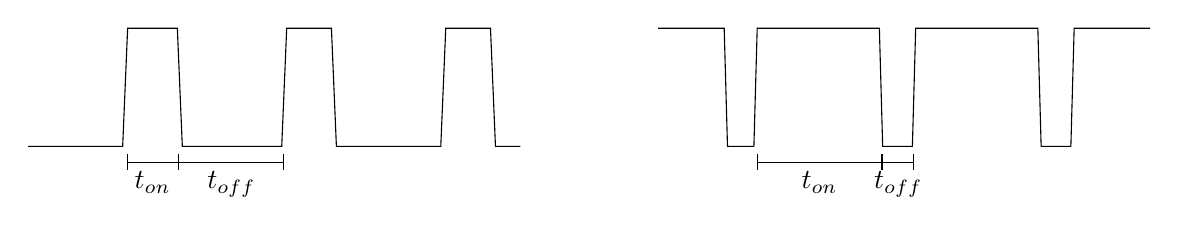
\begin{tikzpicture}
        \draw[domain=0.75:7,variable=\x,samples=100]
            plot ({\x},{(Mod(\x*0.5, 1) < 0.33) * 1.5});
        \draw [|-|] (2,-0.2) -- node[midway,below] {$t_{on}$} (2.66,-0.2);
        \draw [-|] (2.66,-0.2) -- node[midway,below] {$t_{off}$} (4,-0.2);

        \draw[domain=0.75:7,variable=\x,samples=150]
            plot ({\x+8},{(Mod(\x*0.5, 1) < 0.80) * 1.5});
        \draw [|-|] (10,-0.2) -- node[midway,below] {$t_{on}$} (11.6,-0.2);
        \draw [-|] (11.6,-0.2) -- node[midway,below] {$t_{off}$} (12,-0.2);
    \end{tikzpicture}
    \caption{Verlauf zweier PWM-Signale mit gleicher Frequenz, aber
        unterschiedlichem Duty-Cycle. Der Duty-Cycle ergibt sich aus dem
        Verhältnis $\frac{t_{on}}{t_{off}}$ (im linken Signal ca. 33\%, im
        rechten 80\%). Die Periode eines Signals beträgt $t_{on} + t_{off}$ und
        die Frequenz $\frac{1}{t_{on} + t_{off}}$.}
    \label{fig:pwm-signal}
\end{figure}
% TODO: Caption besser in den Text schieben?

% Vllt.: Ausnutzung Trägheit des Motors, des Auges bei LEDs.

Pulsweitenmodulation (PWM) ist ein Modulationsverfahren zum Kodieren analoger
Werte in digitalen Signalen. Dabei wird ein digitaler Ausgang mit einer festen
Frequenz an- und ausgeschaltet. Der kodierte Wert ist der sogenannte
"`Duty-Cycle"' des PWM-Signals und beschreibt das Verhältnis zwischen der An-
und der Aus-Zeit des Signals. Ist der Duty-Cycle 0.0, so ist das resultierende
Signal dauerhaft auf dem niedrigen Pegel (Verbraucher ist ausgeschaltet). Bei
einem Duty-Cycle von 1.0 ist das Signal dauerhaft auf dem hohen Pegel
(Verbraucher ist eingeschaltet). Ein Beispiel eines PWM-Signals ist in
\autoref{fig:pwm-signal} zu sehen. PWM kann genutzt werden, um eine variable
Energiemenge an einen elektrischen Verbraucher zu leiten.

Um ein pulsweitenmoduliertes Signal zu erzeugen, gibt es mehrere Möglichkeiten:

Verfügt die Hardware über einen PWM-Controller so kann dieser programmiert
werden um ein PWM-Signal zu generieren. Ist der Controller konfiguriert,
geschieht die Erzeugung des PWM-Signals im Hintergrund ohne Intervention der
Software. Zur Anpassung des Duty-Cycle ist lediglich nötig, den neuen Wert in
den Controller zu schreiben.

Beim Software-PWM wird der Zustand des gesteuerten Pins per Software geändert,
nachdem die $t_{on}$- bzw. $t_{off}$-Zeit abgelaufen ist. Eine beispielhafte
Implementierung in C-ähnlichem Pseudocode ist im folgenden Listing zu sehen:

\begin{minipage}{\linewidth}
\begin{lstlisting}[
    language=C
]
    // duty = Duty-Cycle (0.0 bis 1.0)
    // freq = PWM-Frequenz in Hertz
    while (true)
    {
        output_on();
        t_on = duty * (1.0 / freq);
        sleep(t_on);

        output_off();
        t_off = (1.0 - duty) * (1.0 / freq);
        sleep(t_off);
    }
\end{lstlisting}
\end{minipage}

Übliche PWM-Frequenzen liegen im Bereich einiger Kilohertz, woraus eine Periode
von einigen hundert Mikrosekunden resultiert. Um beispielsweise einen Duty-Cycle
von 10\% bei einer PWM-Frequenz von 1 kHz zu erzielen, ergibt sich eine An-Zeit
von $t_{on} = {10 \over 100} * {1 \over 1 kHz} = 100 \mu s$ und eine Aus-Zeit
von $t_{off} = (1 - {10 \over 100}) * {1 \over 1 kHz} = 900 \mu s$. Dermaßen
geringe Wartezeiten sorgen dafür, dass Software-PWM meist sehr viel CPU-Zeit
benötigt.

Da der genutzte Raspberry Pi 2B über einen PWM-Controller mit 2 PWM-Kanälen
verfügt, wäre es möglich, diesen für die Motorsteuerung zu nutzen. Allerdings
werden beide Kanäle auch bei der Audiowiedergabe benötigt
\cite{pi-audio-uses-pwm}. Zusätzlich verfügen die älteren Raspberry Pi Modelle
über einen kleineren Header mit nur 26 statt 40 Pins, auf dem nur ein PWM-Kanal
vorliegt \cite{pi-gpio-pinout}. Um größtmögliche Kompatibilität mit anderer
Software die auf dem Raspberry Pi läuft (und möglicherweise Gebrauch von
Audiowiedergabe macht) zu gewährleisten, und um nicht von der spezifischen
PWM-Hardware abhängig zu sein, kommt statt der PWM-Hardware die Softwarelösung
\code{pigpio} zum Einsatz.


\subsection{pigpio}

\newcommand{\pigpio}[0]{\code{pigpio}}

Die \pigpio{}-Bibliothek stellt eine Reihe von Funktionen bereit, mit denen sich
die GPIO-Pins eines Raspberry Pis steuern und lesen lassen. \pigpio{} ermöglicht
sowohl die Steuerung einzelner Pins, als auch die Software-Emulation eines
Buses.

\pigpio{} ermöglicht unter anderem die Verwendung von "`hardware timed PWM"' auf
allen GPIO-Pins \cite{pigpio-web}. Dabei handelt es sich um eine hybride Lösung
aus Soft- und Hardware-PWM, die eine einstellbare Auflösung bis zu einzelnen
Mikrosekunden ermöglicht.

Dazu verwendet \pigpio{} den DMA-Controller des Prozessors
\cite{bcm2835-peripherals}. Mittels DMA (Direct Memory Access) lässt sich ein
Datentransfer starten, der von der Hardware im Hintergrund abgearbeitet wird,
ohne dass sich die CPU oder die darauf laufende Software einschalten muss.
\pigpio{} berechnet die Zustände aller Pins mit der eingestellten Auflösung vor
und speichert sie in einem Puffer. Dann wird der DMA-Controller des Raspberry
Pis so konfiguriert, dass die Pinzustände in die entsprechenden Ausgaberegister
des GPIO-Controllers geschrieben werden. Der Schreibvorgang wird angestoßen,
indem ein freier Timer regelmäßig ein DMA-Event auslöst. Die Größe des Puffers
ist einstellbar und beeinflusst den Arbeitsspeicherverbrauch. Standardmäßig
werden Pinzustände über 120 Millisekunden im Puffer gespeichert, was in einer
maximalen RAM-Nutzung von 16 MB resultiert (bei einer Auflösung von $1 \mu s$)
\cite{pigpio-gpioCfgBufferSize}.

Während die Zustände der GPIO-Pins in Software vorberechnet sind, geschieht ihre
Ausgabe ohne Intervention jeglicher Software, sobald DMA-Controller und Timer
konfiguriert sind. Da der Timer eine Hardwarekomponente ist, nennt der Autor von
\pigpio{} dies "`hardware timed PWM"'.

Dieser Direktzugriff auf Hardwarekomponenten erfordert Zugriff auf
\path{/dev/mem}, eine Gerätedatei, die Operationen direkt auf dem physischen
Speicher des Computers durchführt (zum physischen Speicher zählen hier auch
Peripheriebausteine wie der GPIO- oder DMA-Controller) \cite{dev-mem}. Für
diesen Zugriff werden root-Rechte benötigt.

Die Berechnung der Pinzustände benötigt im Vergleich zu oben beschriebenen
reinen Software-PWM weniger CPU-Ressourcen. Die benötigte Rechenleistung hängt
von der Auflösung des PWM-Signals ab. Der \pigpio{}-Autor gibt Werte von 10-25\%
CPU-Auslastung bei Auflösungen von jeweils 5-1 Mikrosekunden an
\cite{pigpio-gpioCfgClock}.

% TODO refs: https://github.com/raspberrypi/linux/blob/rpi-4.4.y/arch/arm/boot/dts/overlays/README#L934-L935


\subsection{Zugriff aus C++}
\label{subsection:motor-c++}

Da \pigpio{} eine C-Bibliothek ist, aber aus C++-Code heraus genutzt werden
soll, wurde eine Wrapperklasse geschrieben, die die Verwendung vereinfacht. Sie
befindet sich in \path{src/PiGPIO.hpp} und \path{src/PiGPIO.cpp} und erlaubt den
Zugriff auf einzelne Pins mittels der \code{Pin}-Klasse. Es werden nicht alle
Funktionen von \pigpio{} unterstützt, sondern nur eine Untermenge, die zum
Steuern der Motoren ausreichend ist. Dazu zählen die Konfiguration der
PWM-Parameter, das Konfigurieren der Pins als Outputs oder Inputs, das Setzen
des Logiklevels, sowie das Starten von PWM mit gegebenem Duty-Cycle.

Die Motoren werden gesteuert durch die \code{Motor}-Klasse, die in
\path{src/Motor.hpp} definiert ist. Zum Erstellen einer \code{Motor}-Instanz
wird eine \code{MotorConfig} benötigt, die diverse Parameter des Motors festlegt
und aus dem Launch-File \code{launch/kurt.launch} gelesen wird.

Wie am Ende von \autoref{section:Motortreiber} erklärt, verfügen die
Motortreiber nicht über eingebaute Hardware um eine Totzeit der Transistoren
sicherzustellen. Aus diesem Grund begrenzt die \code{Motor}-Klasse die maximale
Anzahl an Richtungsänderungen die ein Motor pro Sekunde durchführen kann.

Zusätzlich wird auch die Maximalbeschleunigung der Motoren von dieser Klasse
begrenzt, um hohe Stromspitzen zu vermeiden. Wird beispielsweise ein Motor aus
dem Stand sofort mit maximalem Duty-Cycle betrieben, fließt ein hoher Strom, der
zum Einbruch der Versorgungsspannung führen kann. Dieser Spannungsabfall kann
dazu führen, dass der Raspberry Pi keine ausreichende Spannung vom
Spannungsregler erhält und abstürzt. Dies hat bei der Arbeit am Roboter ein
signifikantes Problem dargestellt. Wird der Roboter nicht mit einem Akku,
sondern über ein träges Labornetzgerät versorgt, passieren diese Abstürze noch
einfacher.

Die Konfigurationsparameter der \code{Motor}-Klasse sind in \path{src/Motor.hpp}
sowie im Launch-File \path{launch/kurt.launch} umfassend dokumentiert.

Wurde eine Instanz der \code{Motor}-Klasse erstellt, kann mit der Methode
\code{set} eine neue Zielgeschwindigkeit als \code{float} im Bereich $-1.0$ bis
$1.0$ festgelegt werden, wobei $-1.0$ für die Höchstgeschwindigkeit mit
umgekehrter Drehrichtung (rückwärts) steht, und $1.0$ entsprechend für die
Höchstgeschwindigkeit vorwärts. Dabei ist zu beachten, dass die
\code{Motor}-Klasse damit noch keinen geschlossenen Regelkreis erzeugt und die
Geschwindigkeitswerte je nach Gewicht des Roboters und Ladezustand des Akkus
in verschiedenen tatsächlichen Geschwindigkeiten resultieren können.

Das bloße Setzen einer Zielgeschwindigkeit sorgt noch nicht dafür, dass diese
auch angesteuert wird. Dazu muss in regelmäßigen Zeitintervallen die
\code{update}-Methode aufgerufen werden, die die konfigurierten Limits für
Beschleunigung und Richtungswechsel umsetzt und die Motorgeschwindigkeit langsam
an den Zielwert anpasst.


\section{Encoderanbindung}

Zum Lesen der Encodersignale gibt es mehrere Möglichkeiten. Die einfachste
Lösung besteht darin, die Callback-Funktionalität von \pigpio{} zu nutzen um bei
Änderungen auf einem der Encoderkanäle benachrichtigt zu werden (Auswertung in
Software). Eine Python-Implementierung dieses Ansatzes ist in
\path{scripts/encoder.py} zu finden. Der \pigpio{}-Autor stellt einen solchen
Softwareansatz auch als Beispiel bereit \cite{encoder-software-pigpio}. Generell
lassen sich viele äquivalente Implementierungen in diversen Programmiersprachen
im Internet finden \cite{encoder-software-modmypi}
\cite{encoder-software-arduino}.

Dieser Ansatz funktioniert nur bei sehr geringen Geschwindigkeiten zuverlässig,
da bei höheren Geschwindigkeiten die Frequenz der Signale zu schnell wird, um
bei jeder Taktflanke die erforderliche Logik zuverlässig auszuführen. Dem kann
entgegengewirkt werden, indem eine schnellere Programmiersprache für die
Auswertung genutzt würde (beispielsweise C). Allerdings ist auch dies keine
vollständige Lösung des Problems, da der zeitkritische Code noch immer vom
Linux-Scheduler gestartet werden muss, sobald sich das Encodersignal ändert.

Eine mögliche Lösung wäre es, einen Echtzeitkernel zu nutzen, mit dem die Latenz
zwischen dem Zustandswechsel des Signals und der Ausführung des Callbacks
minimiert werden würde. Da das Design eines echtzeitfähigen Systems sowie die
Arbeit mit einem echtzeitfähigen Linux-Kernel eher kompliziert ist (Ubuntu
bietet \emph{fünf} Kernel mit unterschiedlichen Echtzeitfähigkeiten an
\cite{ubuntu-realtime}), wurde nach einer anderen Lösung gesucht, die keinen
Echtzeitkernel erfordert.

Alternativ könnte man \pigpio{} verwenden, um die Encodersignale mit hoher
Samplerate via DMA zu lesen. \pigpio{} stellt dafür die Funktion
\code{gpioSetGetSamplesFunc} zur Verfügung, mit der ein Callback registriert
werden kann, der dann mit den gesammelten Samples aufgerufen wird.

Die Wahl fiel letztlich auf einen anderen Ansatz, der die Latenz des
Linux-Schedulers vollständig umgeht und keinen zeitkritischen Code im Userspace
ausführt: Der Linux-Kernel verfügt bereits über einen generischen Treiber für
Encoder, \code{rotary-encoder}, der Hardwareinterrupts nutzt und vollständig im
Kernel läuft \cite{rotary-encoder}. Bei einer Änderung des Encodersignals wird
ein Interrupt ausgelöst, der über wenige Umwege zum
\code{rotary-encoder}-Treiber gelangt und dort behandelt wird. Der Treiber
bestimmt die Drehrichtung und führt einen Zähler, der über die \code{evdev}-API
an Anwendungen zur Verfügung gestellt wird.
% TODO: User/Kernelspace erklären
% TODO: SPI-Missbrauch

Das \code{evdev}-Interface wird von vielen anderen Ereignis-basierten Geräten
wie Tastaturen, Mäusen und Gamepads verwendet, weshalb es gut dokumentiert und
aus vielen Programmiersprachen einfach zu nutzen ist. Das oben erwähnte
Python-Skript (\path{scripts/encoder.py}) unterstützt auch den Zugriff auf einen
Encoder, der via \code{evdev} eingebunden ist. Es ist auch möglich, die vom
Treiber gesendeten Ereignisse mit dem \code{evtest}-Tool einzusehen, ohne von
spezieller Software abhängig zu sein \cite{evtest-man}.

Zum Laden des Treibers und zum Konfigurieren der GPIO-Pins, an denen die Encoder
angeschlossen sind, wurde die Devicetree-Funktionalität von Linux genutzt, die
im Folgenden genauer beschrieben werden soll.


\subsection{Devicetree}
\label{subsec:devicetree}

\begin{framed}
Bemerkung: Es gibt eine Diskrepanz bei der Schreibweise von "`Devicetree"'.
Während die offizielle Spezifikation \cite{devicetree-spec} immer "`Devicetree"'
als ein einzelnes Wort schreibt, wird das Wort in der Dokumentation im
Linux-Kernel \cite{devicetree-in-linux} als "`Device Tree"' getrennt
geschrieben. Diese Arbeit hält sich an die Schreibweise in der Spezifikation.
\end{framed}

Der Devicetree ist eine Datenstruktur zur Hardwarebeschreibung. Ein Devicetree
kann während des Bootvorganges vom Linux-Kernel geladen werden, um die darin
spezifizierten Geräte und Controller zu konfigurieren und passende Treiber zu
laden \cite{devicetree-in-linux}. Der Devicetree bildet eine Hierarchie aus
Knoten, die Geräte, Controller oder Prozessoren repräsentieren können und sie
mit Eigenschaften versehen können, die von den entsprechenden Treibern zur
Konfiguration genutzt werden können. Beispielsweise lässt sich ein Controller
für den I$^2$C-Bus darstellen, an dem ein Temperatursensor angeschlossen ist,
der im Devicetree als Kindknoten des Controllers aufgeführt ist.

Der aktuelle Devicetree eines Linux-Systems ist im virtuellen Ordner
\path{/proc/device-tree} als Dateihierarchie einsehbar. Nutzt das System keinen
Devicetree, so existiert der Ordner nicht.

Um diese Datenstruktur zu erstellen, ist eine Syntax spezifiziert, mit der ein
menschenlesbarer Devicetree erstellt werden kann. Die Syntax kann mit anderen
Datenbeschreibungssprachen wie JSON verglichen werden. Für solchen
Devicetree-Quellcode wird per Konvention die Dateiendung \code{.dts} verwendet.

Der Devicetree kann durch sogenannte Overlays erweitert werden, die zusätzliche
Knoten definieren oder bestehende Knoten modifizieren
\cite{devicetree-overlay-notes}. Overlays können zur Bootzeit geladen werden
oder während das System bereits läuft. Ein solches Overlay wird zur Einbindung
der Encoder genutzt.

Die Kompilierung von \code{.dts}-Dateien wird mit dem Devicetree-Compiler
\code{dtc} durchgeführt. Dieser Vorgang ist plattformunabhängig und muss nicht
zwangsläufig auf dem Zielsystem stattfinden: Solange alle inkludierten
\code{.dtsi}-Dateien auf dem System vorhanden sind, kann das Kompilat erstellt
und auf dem beschriebenen System eingesetzt werden. Zusätzlich zum Kompilieren
von Devicetrees und Overlays kann \code{dtc} auch genutzt werden, um bereits
kompilierte \code{.dtb}- und \code{.dtbo}-Dateien wieder in menschenlesbaren
Quellcode umzuwandeln. Auch der aktuell vom System genutzte Devicetree kann
angezeigt werden, indem \path{/proc/device-tree} an den Compiler übergeben
wird.
% TODO: Ausprobieren ohne -@

Zum besseren Verständnis soll \autoref{tbl:devicetree-file-types} einen
Überblick über die verschiedenen Dateitypen verschaffen, die für die Arbeit mit
dem Devicetree verwendet werden.

\begin{table}
    \centering
    \begin{tabular}{|l|l|l|}
        Dateiendung  & Bedeutung & Nutzung       \\ \hline
        \code{.dts}  & Devicetree Source & Quellcode für Devicetree oder Overlay \\
        \code{.dtsi} & Devicetree Source Include & Kann in \code{.dts}-Dateien eingebunden werden \\
        \code{.dtb}  & Devicetree Blob & Kompilierter Devicetree \\
        \code{.dtbo} & Devicetree Blob Overlay & Kompiliertes Overlay  \\
    \end{tabular}
    \caption{
        Übersicht über Dateitypen die für den Devicetree genutzt werden.
    }
    \label{tbl:devicetree-file-types}
\end{table}

Das Overlay für die Encoder ist definiert in \path{kernel/kurt-encoders.dts} und
kann mit dem dort vorhandenen Makefile erstellt, geladen und installiert werden.
Die bereitgestellten Targets sind in \autoref{tbl:devicetree-makefile-target}
aufgeführt.

\begin{table}
    \centering
    \begin{tabular}{|l|p{0.6\linewidth}|}
        Befehl & Bedeutung        \\ \hline

        \code{make} / \code{make build}
        & Kompiliert den Overlay-Quellcode \code{kurt-encoders.dts} zum ladbaren
        Overlay \code{kurt-encoders.dtbo}. \\

        \code{make load}
        & Kompiliert das Overlay und lädt es (dies ist zum Testen gedacht und
        wird durch einen Neustart rückgängig gemacht). \\

        \code{make unload}
        & Entlädt das mit \code{make load} geladene Overlay wieder. \\

        \code{make install}
        & Kompiliert das Overlay und installiert es nach \path{/boot/overlays}
        (benötigt root-Rechte). Hierdurch wird es noch \emph{nicht} automatisch
        geladen. \\

        \code{make uninstall}
        & Löscht das installierte Overlay aus \path{/boot/overlays} (benötigt
        root-Rechte). \\

        \code{make clean}
        & Löscht das kompilierte Overlay (\code{kurt-encoders.dtbo}). \\
    \end{tabular}
    \caption{
        \code{make}-Targets für die Arbeit mit dem Encoder-Overlay.
    }
    \label{tbl:devicetree-makefile-target}
\end{table}

\begin{minipage}{\textwidth}
Damit das Overlay beim Starten des Raspberry Pis automatisch geladen wird,
musste der folgende Eintrag am Ende der Datei \path{/boot/config.txt}
hinzugefügt werden:

\begin{lstlisting}[numbers=none]
    dtoverlay=kurt-encoders
\end{lstlisting}
\end{minipage}

% TODO: Ausprobieren:
Es ist zu beachten, dass das Laden des Overlays zur Laufzeit nur möglich ist,
wenn keine alte Version des Overlays während des Bootvorganges geladen wurde.
Praktisch bedeutet dies, dass \code{make load} nur ausgeführt werden darf,
nachdem die \code{dtoverlay}-Zeile auskommentiert und das System neu gestartet
wurde.

Die Arbeit mit dem Devicetree ist oft komplex, da sehr viele interagierende
Module und Gerätetreiber verwaltet werden müssen und \code{dtc} oft nur wenig
hilfreiche Fehler und Warnungen bereitstellt. Aus diesem Grund soll im Folgenden
das im Rahmen dieser Arbeit entwickelte Devicetree-Overlay für die Encoder in
seiner Vollständigkeit erklärt werden.

\begin{lstlisting}[
    caption={
        Vereinfachte Version des Devicetree-Overlays in
        \code{kernel/kurt-encoders.dts} für die Encoder des KURT2-Roboters.
        Basierend auf \cite{rotaries-overlay} und \cite{devicetree-tutorial}.
    },
    label=lst:devicetree-overlay,
    language=C,
    alsoletter=-/|,
    alsoother=@,
    float,
    morekeywords={
        /dts-v1/,
        /plugin/,
        fragment,
        compatible,
        pins,
        function,
        pull,
        __overlay__,
        target,
        pinctrl-0,
        pinctrl-names,
        gpios
    }
]
    /dts-v1/;
    /plugin/;

    / {
        compatible = "brcm,bcm2708";

        fragment@0 {
            target = <&gpio>;
            __overlay__ {
                rot_left_pins: rot_left_pins {
                    brcm,pins = <21 20>;
                    brcm,function = <0>;
                    brcm,pull = <0>;
                };

                rot_right_pins: rot_right_pins {
                    brcm,pins = <11 10>;
                    brcm,function = <0>;
                    brcm,pull = <0>;
                };
            };
        };

        fragment@1 {
            target = <&soc>;
            __overlay__ {
                rot_left: rot_left {
                    compatible = "rotary-encoder";
                    pinctrl-names = "default";
                    pinctrl-0 = <&rot_left_pins>;
                    gpios = <&gpio 21 0>, <&gpio 20 0>;
                    linux,axis = <0>;   // REL_X / ABS_X
                    rotary-encoder,rollover;
                    rotary-encoder,steps = <100000>;
                };

                rot_right: rot_right {
                    compatible = "rotary-encoder";
                    pinctrl-names = "default";
                    pinctrl-0 = <&rot_right_pins>;
                    gpios = <&gpio 11 0>, <&gpio 10 0>;
                    linux,axis = <0>;   // REL_X / ABS_X
                    rotary-encoder,rollover;
                    rotary-encoder,steps = <100000>;
                };
            };
        };
    };
\end{lstlisting}

% TODO: Node-Label unnötig?

Das in \autoref{lst:devicetree-overlay} gezeigte Overlay beginnt mit 2
Direktiven an den Compiler. Die erste, \code{/dts-v1/}, legt die Version der
Devicetree-Sprache fest. Momentan existiert nur Version 1. Die zweite Direktive,
\code{/plugin/}, teilt dem Compiler mit, dass es sich bei dieser Datei um ein
Overlay statt einen eigenständigen Devicetree handelt.

Mit dem \code{/}-Knoten in Zeile 4 (der Wurzel) beginnt das eigentliche Overlay.
Der Wurzelknoten hat eine Eigenschaft, \code{compatible}, die in Zeile 5 auf den
String \code{"brcm,bcm2708"} festgelegt wird. Damit wird dieses Overlay mit dem
BCM2708-Chip von Broadcom als kompatibel gekennzeichnet. BCM2708 ist die
Prozessorfamilie des ersten Raspberry Pis, mit der alle Nachfolgermodelle
kompatibel sind. Der hier verwendete Raspberry Pi 2B nutzt beispielsweise ein
SoC der BCM2709-Familie. Somit markiert dies das Overlay als kompatibel mit
allen Raspberry Pis.

Das Overlay besteht aus 2 Fragmenten, die jeweils einen anderen Teil des
Devicetrees modifizieren. Ein Fragment definiert eine \code{target}-Eigenschaft,
die ein sogenanntes \code{phandle} als Wert zugewiesen bekommt. Ein
\code{phandle} ist eine Referenz auf einen anderen (bestehenden) Knoten im
Devicetree. Mit der \code{target}-Eigenschaft wird der Zielknoten des Fragments
festgelegt, der erweitert oder modifiziert werden soll. Der dem Fragment
untergeordnete \code{\_\_overlay\_\_}-Knoten wird dann genutzt, um seine
Kindknoten und Eigenschaften in den als \code{target} definierten Knoten zu
injizieren.

Das erste Fragment, \code{fragment@0}, hat als \code{target} den Knoten
\code{gpio}. Der \code{gpio}-Knoten ist nicht im Overlay definiert, sondern im
Devicetree des Raspberry Pis. Er kann eingesehen werden, indem der aktuelle
Devicetree auf einem Raspberry Pi mittels \code{dtc /proc/device-tree} angezeigt
wird. Die Definition des Knotens befindet sich im Linux-Quellcode in
\path{arch/arm/boot/dts/bcm283x.dtsi} \cite{devicetree-pi-gpio}. Die dort
enthaltene Zeile \code{compatible = "brcm,bcm2835-gpio";} sorgt dafür, dass der
\code{brcm,bcm2835-gpio}-Treiber für den GPIO-Controller genutzt wird
\cite{devicetree-bcmgpio}. Der im Fragment enthaltene
\code{\_\_overlay\_\_}-Knoten definiert 2 Knoten, die dem \code{gpio}-Knoten als
Kindknoten hinzugefügt werden sollen: \code{rot\_left\_pins} und
\code{rot\_right\_pins}.

Beide hinzugefügten Knoten definieren jeweils eine Pingruppe, die vom
\code{pinctrl}-Subsystem des Kernels verwaltet wird. \code{pinctrl} erlaubt es,
mehrere Pins zu logischen Gruppen zu kombinieren und ihre Konfiguration
gemeinsam zu definieren. Viele GPIO-Controller erlauben beispielsweise die
Auswahl einer von mehreren Funktionen, die ein Pin erfüllen soll, sowie die
Konfiguration von integrierten Pull-Up und/oder Pull-Down Widerständen. Der
bereits vorhandene \code{gpio}-Knoten enthält bereits viele vordefinierte
Pingruppen, die von Hardwareperipherie genutzt werden können
\cite{devicetree-pi-gpio}.

Beide Pingruppen definieren die gleichen 3 Eigenschaften:

\begin{itemize}
    \item \code{brcm,pins} listet die Pins auf, die Teil der Gruppe sind.

    Die Reihenfolge spielt keine Rolle, aber aus Gründen der Konsistenz wird
    zuerst der Pin des A-Kanals und dann der des B-Kanals des Encoders
    aufgeführt. Beide Gruppen unterscheiden sich ausschließlich durch die Pins,
    die ihnen zugeordnet sind, alle nachfolgenden Eigenschaften sind identisch.

    \item \code{brcm,function} selektiert, welche interne Funktion auf den Pin
    gelegt werden soll.

    Der hier gewählte Wert 0 konfiguriert die Pins als Inputs. Mit dem Wert 1
    könnte man sie als Outputs konfigurieren und Werte von 2-7 legen sogenannte
    "`alternate functions"' auf den Pin, die von anderer Peripherie zur
    Verfügung gestellt wird \cite{devicetree-bcmgpio}.

    \item \code{brcm,pull} konfiguriert die integrierten Pull-Up und Pull-Down
    Widerstände.

    Der Wert 0 deaktiviert die Widerstände, da die genutzten Encoder sie nicht
    benötigen. Sollen andere Encoder genutzt werden, muss dieser Wert unter
    Umständen geändert werden. Andere gültige Werte für die
    \code{brcm,pull}-Eigenschaft wären 1, um den Pull-Down Widerstand zu
    aktivieren, oder 2, um den Pull-Up Widerstand zu nutzen
    \cite{devicetree-bcmgpio}.
\end{itemize}

Die bloße Definition dieser 2 Pingruppen hat alleine noch keinen Effekt. Die
Gruppen müssen erst von einem anderen Devicetree-Knoten genutzt werden, damit
sich ihre Einstellungen auswirken. Dies geschieht im zweiten Fragment des
Overlays, \code{fragment@1}.

Zeile 25 legt als Zielknoten \code{soc} fest. Dieser Knoten ist ebenfalls in der
Datei \path{arch/arm/boot/dts/bcm283x.dtsi} definiert und ist der Elternknoten
der gesamten Peripherie des Broadcom-SoCs. Auch dieses Fragment fügt wieder 2
neue Knoten ein, ohne bestehende zu verändern. Wieder unterscheiden sich beide
nur durch ihren Namen und die zugewiesenen GPIOs, weshalb nur auf den ersten
Knoten, \code{rot\_left}, genauer eingegangen wird, der den Encoder des linken
Motors darstellt.

Folgende Eigenschaften werden festgelegt:

\begin{itemize}
    \item \code{compatible = "rotary-encoder";}

    Diese Zeile teilt dem Devicetree-Subsystem mit, dass das durch diesen Knoten
    beschriebene Gerät mit dem \code{rotary-encoder}-Treiber kompatibel ist, der
    beim Laden des Overlays nun vom Kernel geladen wird, um das Gerät
    anzusprechen.

    \item \code{pinctrl-names = "default";}

    Hier werden die Pinzustände, in denen sich der Gerätetreiber befinden kann,
    benannt. Für die Encoder existiert nur ein Zustand, der nie gewechselt wird,
    aber andere Gerätetreiber könnten beispielsweise einen Pin zwischen Output
    und Input hin- und zurückschalten, um einen bidirektionalen Bus zu
    implementieren.

    \item \code{pinctrl-0 = <\&rot\_left\_pins>;}

    Der einzige Pinzustand der Encoder wird hier festgelegt. Er besteht aus der
    im ersten Fragment definierten Pingruppe \code{rot\_left\_pins}. Für
    komplexere Treiber kann eine beliebige Anzahl Pingruppen zu einem Zustand
    kombiniert werden, aber für die Encoder ist eine Gruppe ausreichend.

    Aufgrund dieser Zeile konfiguriert das \code{pinctrl}-Subsystem die
    verwendeten Pins so um, wie im \code{rot\_left\_pins}-Knoten definiert.

    \item \code{gpios = <\&gpio 21 0>, <\&gpio 20 0>;}

    Mit dieser Zeile wird dem \code{rotary-encoder}-Treiber mitgeteilt, an
    welchen GPIO-Pins die beiden Encoderkanäle angeschlossen sind. Die Pins sind
    identisch mit denen der zugewiesenen Pingruppe, \code{rot\_left\_pins}. Hier
    ist jedoch die Reihenfolge wichtig, da der erste Eintrag als Pin für den
    A-Kanal des Encoders genutzt wird, und entsprechend der zweite Eintrag für
    den B-Kanal.

    Die Syntax der Pinangaben listet zuerst den Devicetree-Knoten des
    GPIO-Controllers via \code{phandle}. Im Falle des Raspberry Pi ist das der
    gleiche Knoten der auch im ersten Fragment zur Definition der Pingruppen
    genutzt wurde (der Pin-Controller, oder \code{pinmux}). GPIO-Controller und
    \code{pinmux} müssen aber nicht zwangsläufig vom selben Knoten repräsentiert
    werden. Die restliche Syntax ist Treiberabhängig. Hier folgt dem
    GPIO-Controller \code{phandle} die Nummer des GPIOs (diese kann dem
    Datenblatt entnommen werden \cite{bcm2835-peripherals}) sowie ein Wert mit
    dem optionale Parameter angegeben werden können. Die optionalen Parameter
    sind hier immer 0, der einzige andere Wert, der akzeptiert wird, ist 1,
    wodurch der Zustand des Pins aus Softwaresicht invertiert werden würde
    \cite{devicetree-bcmgpio}.

    Zusammenfassend legt diese Zeile also GPIO 21 für den A-Kanal und GPIO 20
    für den B-Kanal des Encoders fest.

    \item \code{linux,axis = <0>;}

    Diese Zeile konfiguriert das erzeugte \code{evdev}-Gerät, indem die Achse
    festgelegt wird, über die der Encoderwert übermittelt wird
    \cite{devicetree-rotary}. Gültig sind alle Werte, die das Input-Subsystem
    von Linux als Identifikatoren für Achsen anerkennt \cite{input-event-codes}.

    Der Wert 0 ist dort als die Achse \code{REL\_X} und \code{ABS\_X} definiert.
    Der Encodertreiber nutzt standardmäßig eine absolute Achse, also ist
    \code{ABS\_X} in diesem Fall richtig.

    Indem man die Eigenschaft \code{rotary-encoder,relative-axis} spezifiziert,
    kann stattdessen eine relative Achse erzeugt werden. Diese überträgt nur
    inkrementelle Ereignisse, also würde man beim Drehen des Encoders eine Reihe
    von "`+1"'- bzw. "`-1"'-Ereignissen empfangen. Dann müsste der Code, der den
    Encoder nutzt, aber in der Lage sein, \emph{jedes} der Ereignisse zu
    empfangen und auf einen internen Zähler zu rechnen. Indem der Treiber im
    absoluten Modus betrieben wird, führt er diesen Zähler selbst und berichtet
    dessen Wert als Ereignisse an das Programm. Geht nun ein Ereignis verloren,
    kann dies einfach ignoriert werden und mit dem nächsten Ereignis
    weitergearbeitet werden, ohne dass Zählschritte verloren gehen.

    Zur weiteren Einrichtung des \code{evdev}-Interfaces und der absoluten Achse
    dienen auch die nächsten Zeilen.

    \item \code{rotary-encoder,rollover;}

    Ist die \code{rollover}-Eigenschaft vorhanden, so wird der interne Zähler
    nach Erreichen der oberen oder unteren Begrenzung zum "`überlaufen"'
    gebracht und nimmt den Wert an der gegenüberliegenden Begrenzung an
    \cite{devicetree-rotary}.

    \item \code{rotary-encoder,steps = <100000>;}

    Hier wird die obere Begrenzung des Zählers auf 100000 festgelegt
    \cite{devicetree-rotary}. Das sollte ausreichen, damit die Software den
    Zähler nach weniger als 50000 verpassten Schritten abfragt. Geschieht die
    Abfrage nicht rechtzeitig, so würde die Software errechnen, dass der Encoder
    in die andere Richtung gedreht wurde, wodurch die Odometriedaten stark
    verfälscht werden würden.
    % TODO: Besser erklären

    % TODO: Vllt. rollover und steps tauschen
\end{itemize}

Die erstellten \code{evdev}-Geräte tauchen nach dem Laden des Overlays als
\path{/dev/input/js0} und \path{/dev/input/js1} auf, sofern keine anderen
\code{evdev}-Geräte vor den Encodern registriert wurde.



\subsection{Zugriff aus C++}

Der ROS-Node enthält sowohl Code für den Zugriff auf die durch den
\code{rotary-encoder}-Treiber erstellten \code{evdev}-Geräte, als auch für das
Auslesen in Software mithilfe von \pigpio{}.

Dazu wurde eine simple Klassenhierarchie erstellt, dessen Basisklasse in
\path{src/Encoder.hpp} definiert ist. Die \code{Encoder}-Klasse stellt
Basisfunktionalitäten zur Verfügung, die die rohen Encoderticks in
Radumdrehungen und Winkelgeschwindigkeit umrechnen können. Die einzige Methode,
die eine Subklasse implementieren muss, ist die rein virtuelle Methode \code{int
read()}, die die Anzahl der Encoderticks seit dem letzten Aufruf von
\code{read()} (oder seit dem Erstellen der Klasseninstanz, wenn \code{read()}
zum ersten mal aufgerufen wird) zurückliefern muss.

Die Klasse \code{EvdevEncoder} implementiert den Zugriff auf die
\code{evdev}-Encoder mithilfe von \code{libevdev}, einer C-Bibliothek für den
Zugriff \code{evdev}-Geräte \cite{libevdev}.

Der Konstruktor der Klasse benötigt die folgenden Argumente:

\begin{itemize}
    \item \code{int ticksPerTurn}

    Legt die Anzahl der Encoderticks pro Radumdrehung fest. Dieser Wert wird an
    die zugrundeliegende \code{Encoder}-Klasse übergeben und dort zur Umrechnung
    von Ticks in nützlichere Einheiten genutzt.

    \item \code{const std::string\& search\_name}

    Das Suchmuster für das \code{evdev}-Gerät, das gelesen werden soll.

    Anstatt einfach den vollständigen Pfad zu nutzen, werden alle Gerätedateien,
    deren Pfade mit \path{/dev/input/event*} beginnen, gegen \code{search\_name}
    getestet. Passt genau eine Datei auf das Suchmuster, wird sie als der
    Encoder geöffnet.

    Falls sich nun das Namensschema des \code{rotary-encoder}-Treibers oder des
    Devicetrees ändert, bestehen gute Chancen, dass das richtige Gerät trotzdem
    gefunden wird.

    \item \code{int wrap}

    Der Maximalwert des Encoders. Dieser Wert muss mit dem im Devicetree
    übereinstimmen.

% TODO `wrap` könnte unnötig sein?

    \item \code{bool invert}

    Mit diesem Parameter kann die Drehrichtung des Encoders invertiert werden.
\end{itemize}

% TODO: Realistische Zähler messen.

Die Implementierung der \code{read}-Methode muss auf einen eventuellen Überlauf
(bzw. Unterlauf) des Zählers reagieren können, da sich dieser immer zwischen 0
und dem eingestellten \code{wrap}-Wert bewegt (hier wurde 100000 gewählt). Das
bedeutet, dass auch bei einem sehr hohen Maximalwert im Milliardenbereich ein
Unterlauf des Zählers möglich ist, indem der Encoder einfach rückwärts gedreht
wird.

% TODO: Illustrieren


\section{PID-Regler}

\begin{figure}[h]
    \centering
    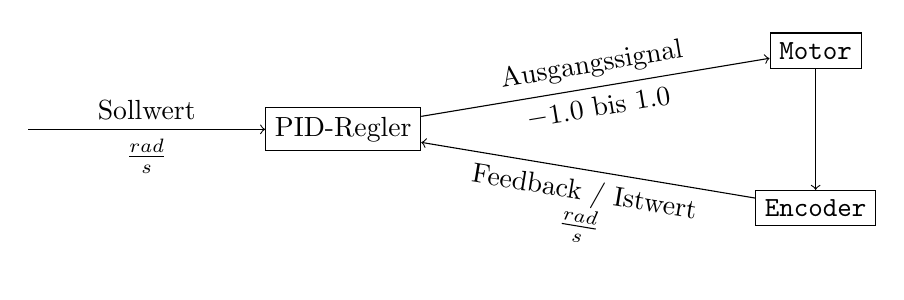
\begin{tikzpicture}
        \node[draw=black] (controller) at (0,0) {PID-Regler};
        \node[draw=black] (actuator) at (6,1) {\code{Motor}};
        \node[draw=black] (sensor) at (6,-1) {\code{Encoder}};

        \draw[->] (controller) -- node[midway,above,sloped] {Ausgangssignal} node[midway,below,sloped] {$-1.0$ bis $1.0$} (actuator);
        \draw[->] (actuator) to (sensor);
        \draw[->] (sensor) to node[midway,below,sloped,align=center] {Feedback / Istwert \\ $rad \over s$} (controller);
        \draw[->] (-4,0) to node[midway,above] {Sollwert} node[midway,below] {$rad \over s$} (controller);
    \end{tikzpicture}
    \caption{
        Schematische Darstellung des verwendeten PID-Reglers. Das
        Ausgangssignal wird an die \code{Motor}-Klasse übergeben, die das
        PWM-Signal erzeugt.
    }
    \label{fig:controller}
\end{figure}

Jetzt, wo die Motoren mit C++-Code gesteuert werden können und die
Radgeschwindigkeit des Roboters abgefragt werden kann, kann mit beidem ein
geschlossener Regelkreis implementiert werden. Dieser erlaubt das Setzen der
Radgeschwindigkeit der linken und rechten Seite des Roboters und hält diese
selbstständig, unabhängig von der Beladung des Roboters und des Ladestands des
Akkus.

Als Regler wird ein generischer PID-Regler verwendet, der in der Datei
\path{src/PIDController.cpp} implementiert ist. Die Interaktionen mit anderen
Teilen der Software sowie die verwendeten physikalischen Einheiten sind in
\autoref{fig:controller} dargestellt. Die Implementierung rechnet ausschließlich
in \code{float}s und ist unabhängig von den tatsächlich vorliegenden Einheiten.

Ein PID-Regler verfügt über 3 Teile, deren gewichtete Summe das Ausgangssignal
des Reglers ist \cite{pid-theory}:

\begin{itemize}
    \item \textbf{P}roportional

    Der Proportionalteil des Reglers entspricht der Abweichung der geregelten
    Größe (hier die Motorgeschwindigkeit) von ihrem Sollwert.

    Besteht ein Regler nur aus einem P-Teil, so spricht man von einem P-Regler.

    \item \textbf{I}ntegral

    Der Integralteil summiert die Abweichung vom Sollwert über mehrere
    Zeitschritte auf.

    Besteht ein Regler nur aus einem I-Teil, so spricht man von einem I-Regler.

    \item \textbf{D}erivative

    Der D-Anteil entspricht der zeitlichen Veränderung des Fehlers (der
    Abweichung vom Sollwert). Steigt die Abweichung vom Sollwert (der Fehler),
    so ist der D-Anteil $> 0$ und erhöht das Ausgangssignal des Reglers. Sinkt
    die Abweichung, so bewegt sich die Größe auf das Ziel zu und der D-Anteil
    wird $< 0$, wodurch das Ausgangssignal des Reglers abgeschwächt wird und das
    Ziel langsamer angesteuert wird. Damit dämpft der D-Anteil den Regler,
    wodurch das Überschreiten des Zielwertes vermindert wird und sich der Regler
    weniger in Oszillation begibt.

    Ein Regler, der nur aus einem D-Teil besteht, kann nicht sinnvoll als Regler
    genutzt werden, da er den Sollwert nicht ansteuert. Wird ein P-Regler mit
    einem D-Anteil verwendet, spricht man von einem PD-Regler.
\end{itemize}

Die Gewichtung des P-, I-, und D-Teiles ist gegeben durch die Faktoren $K_p$,
$K_i$ und $K_d$, die im Launch-File konfiguriert werden können und als Parameter
an den Konstruktor der \code{PIDController}-Klasse übergeben werden.

Zusätzlich kann der I-Anteil auf ein Maximum begrenzt werden. Dieses Limit wird
als Parameter \code{integralLimit} an den Konstruktor übergeben und ist im
Launch-File als \code{windup\_limit} konfigurierbar. Es dient dazu, ein
Überschreiten des Sollwerts aufgrund eines zu hohen Einflusses des I-Anteils zu
vermeiden. Wird $K_i$ auf 0 gesetzt, so hat dieses Limit keinen Effekt (der
Regler wird effektiv zu einem PD-Regler).


\section{ROS-Einbindung}
\label{section:ros-integration}

\begin{figure}
    \centering
    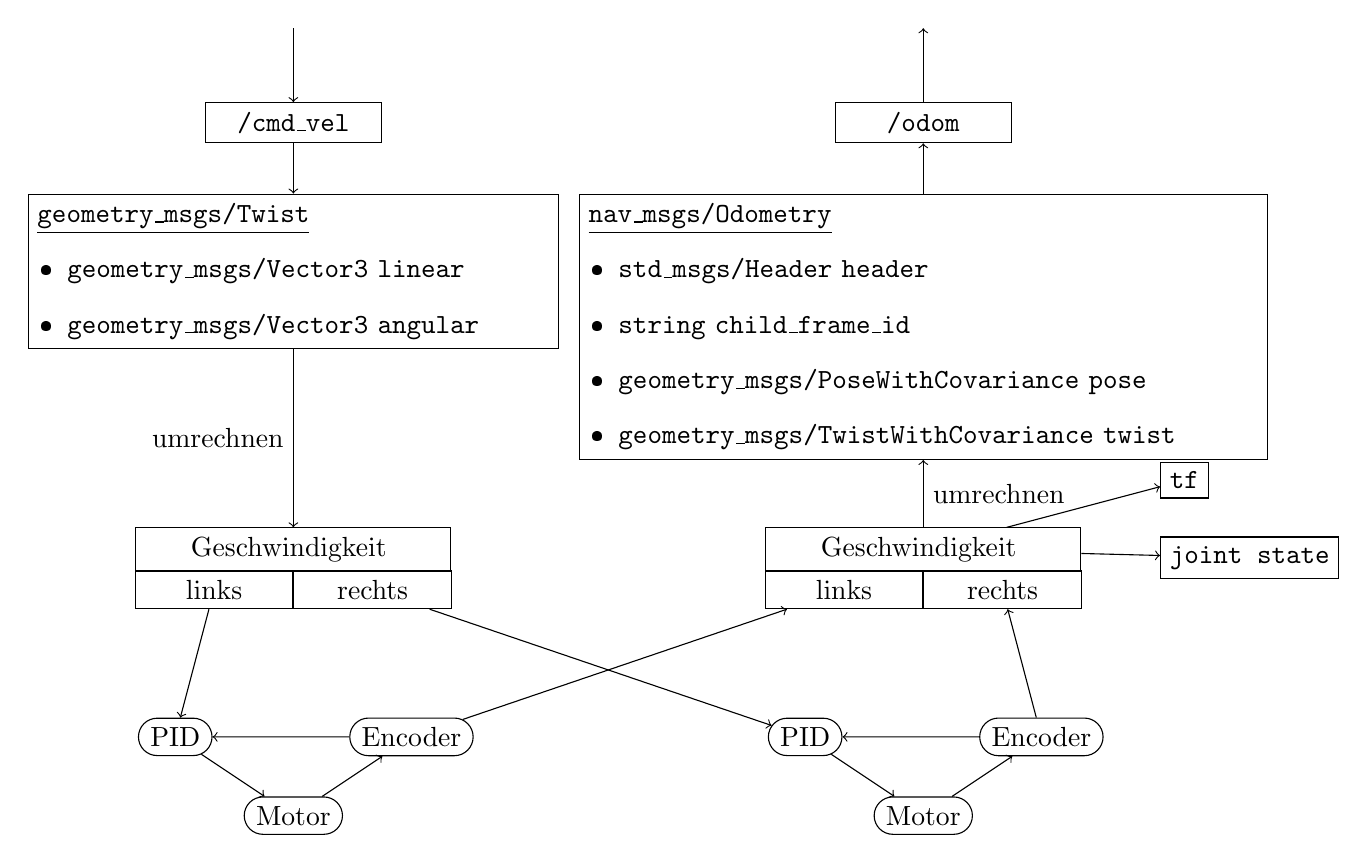
\begin{tikzpicture}
        \node[draw,text width=2cm,align=center] (topic-cmdvel) at (0,5.3) {\code{/cmd\_vel}};
        \node[draw,text width=2cm,align=center] (topic-odom) at (8,5.3) {\code{/odom}};
        \draw[->] (0,6.5) to (topic-cmdvel);
        \draw[<-] (8,6.5) to (topic-odom);

        \node[draw,text width=6.5cm,anchor=north] (msg-twist) at (0,4.4) {
            \underline{\code{geometry\_msgs/Twist}}
            \begin{itemize}
                \setlength{\itemindent} {-.5cm}
                \item \code{geometry\_msgs/Vector3 linear}
                \item \code{geometry\_msgs/Vector3 angular}
            \end{itemize}
        };
        \node[draw,text width=8.5cm,anchor=north] (msg-odometry) at (8,4.4) {
            \underline{\code{nav\_msgs/Odometry}}
            \begin{itemize}
                \setlength{\itemindent} {-.5cm}
                \item \code{std\_msgs/Header header}
                \item \code{string child\_frame\_id}
                \item \code{geometry\_msgs/PoseWithCovariance pose}
                \item \code{geometry\_msgs/TwistWithCovariance twist}
            \end{itemize}
        };

        \draw[->] (topic-cmdvel) to (msg-twist);
        \draw[<-] (topic-odom) to (msg-odometry);

        \node[draw, align=center, minimum width = 4cm,minimum height=0,anchor=south] (spd-left) at (0,-0.4) {
            Geschwindigkeit
        };
        \node[draw, align=center, minimum width=2cm, below=-\pgflinewidth of spd-left, anchor=north east] (spd-left-l) {links};
        \node[draw, align=center, minimum width=2cm, below=-\pgflinewidth of spd-left, anchor=north west] (spd-left-r) {rechts};

        \node[
            draw, align=center,
            minimum width = 4cm, minimum height=0,
            anchor=south
        ] (spd-right) at (8,-0.4) {
            Geschwindigkeit
        };
        \node[draw, align=center, minimum width=2cm, below=-\pgflinewidth of spd-right, anchor=north east] (spd-right-l) {links};
        \node[draw, align=center, minimum width=2cm, below=-\pgflinewidth of spd-right, anchor=north west] (spd-right-r) {rechts};

        \node[draw,right=of spd-right,yshift=25pt] (tf) {\code{tf}};
        \draw[->] (spd-right) -- (tf);

        \node[draw,right=of spd-right,yshift=-3pt] (joint-state) {\code{joint state}};
        \draw[->] (spd-right) -- (joint-state);

        \draw[->] (msg-twist) to node[midway,left] {umrechnen} (spd-left);
        \draw[<-] (msg-odometry) to node[midway,right] {umrechnen} (spd-right);

        \node[rounded rectangle,draw] (pid-left) at (-1.5,-2.5) {PID};
        \node[rounded rectangle,draw] (encoder-left) at (1.5,-2.5) {Encoder};
        \node[rounded rectangle,draw] (motor-left) at (0,-3.5) {Motor};
        \draw[->] (spd-left-l) -- (pid-left);
        \draw[<-] (spd-right-l) -- (encoder-left);
        \draw[->] (encoder-left) -- (pid-left);
        \draw[->] (motor-left) -- (encoder-left);
        \draw[->] (pid-left) -- (motor-left);

        \node[rounded rectangle,draw] (pid-right) at (6.5,-2.5) {PID};
        \node[rounded rectangle,draw] (encoder-right) at (9.5,-2.5) {Encoder};
        \node[rounded rectangle,draw] (motor-right) at (8,-3.5) {Motor};
        \draw[->] (spd-left-r) -- (pid-right);
        \draw[<-] (spd-right-r) -- (encoder-right);
        \draw[->] (encoder-right) -- (pid-right);
        \draw[->] (motor-right) -- (encoder-right);
        \draw[->] (pid-right) -- (motor-right);
    \end{tikzpicture}
    \caption{
        Datenfluss zwischen ROS und den PID-Reglern. Die Umwandlung der
        übertragenen Nachrichten wird von \code{ros\_control} übernommen.
        Nachrichtenstruktur nach \cite{ros-twist} und \cite{ros-odometry}.
    }
    \label{fig:ros-dataflow}
\end{figure}

Nun ist die Software in der Lage, die Radgeschwindigkeiten auf beiden Seiten des
Roboters zu regeln und die aktuelle Geschwindigkeit auszulesen. Damit all das in
ROS integriert werden kann, müssen die Standardschnittstellen von ROS
unterstützt werden, die im Folgenden erklärt werden sollen.

Die Steuerung eines Roboters wird üblicherweise über das Topic \code{/cmd\_vel}
durchgeführt. Ein ROS-Node kann dort Nachrichten vom Typ
\code{geometry\_msgs/Twist} veröffentlichen, um den Roboter anzuweisen, sich zu
bewegen \cite{ros-twist}. Damit dies funktioniert, muss die Software als
Subscriber auf solche Nachrichten reagieren.

Eine \code{Twist}-Nachricht enthält die gewünschte lineare Geschwindigkeit sowie
die Winkelgeschwindigkeit aus Sicht des Roboters. Diese Geschwindigkeiten müssen
in die Geschwindigkeiten des linken und rechten Motors des Differentialantriebs
umgerechnet werden, bevor der Sollwert des Reglers gesetzt werden kann.

Die vollständige Integration der Odometriedaten ist weitaus komplizierter als
die Steuerung des Roboters via \code{/cmd\_vel}. Die Odometriedaten werden
zunächst als Nachrichten vom Typ \code{nav\_msgs/Odometry} über das
\code{/odom}-Topic veröffentlicht \cite{ros-odometry}. Auch hier müssen die
Daten zunächst in eine \code{Odometry}-Nachricht konvertiert werden. Zusätzlich
müssen die Odometriedaten aber auch an das \code{tf}-Subsystem weitergeleitet
werden und die Gelenkzustände aktualisiert werden. Warum das nötig ist, soll in
den nachfolgenden Abschnitten erklärt werden.

\autoref{fig:ros-dataflow} verdeutlicht den Datenfluss zwischen ROS und dem
Rest des Softwarestacks.


\subsection{tf}

Das \code{tf}-Paket (kurz für "`Transform"') erlaubt die Definition von
verknüpften Koordinatensystemen ("`Frames"'), zwischen denen dann effizient
umgerechnet werden kann \cite{ros-tf}. Die Koordinatensysteme bilden eine
Baumstruktur, in der ein Kindknoten relativ zum Elternknoten durch Anwendung
einer Translation und Rotation definiert wird.

Die Koordinatensysteme können sich zur Laufzeit dynamisch ändern, sodass
beispielsweise ein sich drehender Roboterarm dafür sorgt, dass sich das
Koordinatensystem des daran befindlichen Greifers im Verhältnis zur stationären
Welt bewegt.

Ein beweglicher Roboter wie der KURT2 definiert üblicherweise ein
Basiskoordinatensystem \code{/base\_link}, dessen Ursprung das Rotationszentrum
des Roboters ist, sowie ein statisches Koordinatensystem \code{/map}, in dem die
Umgebung des Roboters abgebildet werden kann. Als Kindknoten von
\code{/base\_link} werden oft weitere Koordinatensysteme für Sensoren und
bewegliche Komponenten des Roboters definiert. Für den hier genutzten
KURT2-Roboter sind dynamische Koordinatensysteme für die 6 Räder definiert.

Das \code{tf}-Paket stellt auch einige Tools zum Debuggen der
\code{tf}-Konfiguration bereit: Der aktuelle Zustand des \code{tf}-Baumes lässt
sich mit dem \code{rqt\_tf\_tree}-Tool visualisieren \cite{rqt-tf-tree}. Mit dem
im \code{tf}-Paket enthaltenen Tool \code{tf\_echo} lässt sich die
Transformation zwischen zwei Frames anzeigen (relative Distanz und Rotation)
\cite{ros-tf}.


\subsection{URDF}

URDF (Unified Robot Description Format) ist ein XML-basiertes Format zur
Beschreibung von Robotern \cite{ros-urdf}. Eine URDF-Datei kann
\code{tf}-Koordinatensysteme, bewegliche Gelenke, 3D-Meshes und physikalische
Eigenschaften von Komponenten des Roboters definieren.

Da der ROS-Node zur Steuerung der Originalhardware bereits eine vollständige
URDF-Datei enthält, mussten nur wenige Pfadänderungen daran vorgenommen werden,
damit externe Dateien gefunden werden konnten. Die angepasste URDF-Datei
befindet sich in \path{urdf/kurt_indoor.urdf.xacro}. Die anderen URDF-Dateien im
\code{urdf}-Ordner definieren andere KURT2-Varianten oder werden in die
Hauptdatei eingebunden und sind hier nicht weiter von Belang.

Die URDF-Datei definiert unter anderem Gelenke für die 6 Räder, die sich um ihre
eigene Achse drehen können. Der Zustand dieser Gelenke muss durch die
Odometriedaten aktualisiert werden. Das Launch-File \path{launch/kurt.launch}
startet einen \code{robot\_state\_publisher} ROS-Node, der aus den
Gelenkzuständen dann die entsprechenden Auswirkungen auf den \code{tf}-Tree zu
bestimmen und zu veröffentlichen \cite{ros-robot-state-publisher}. Zusätzlich
veröffentlicht der \code{robot\_state\_publisher} auch alle \code{tf}-Frames,
die fixiert sind und sich \emph{nicht} abhängig von Gelenkzuständen verändern
können. Damit wird der Software die gesamte Arbeit mit dem \code{tf}-Paket
abgenommen: Es müssen lediglich die Gelenkzustände berechnet und gesetzt werden.

Der Inhalt der URDF-Datei wird als Parameter \code{robot\_description} im
Launch-File \path{launch/kurt.launch} eingebunden und steht damit allen Nodes
zur Verfügung.


\subsection{ros\_control}

Um die Interaktion mit \code{/cmd\_vel} und \code{/odom} einfacher zu gestalten,
wurden die \code{ros\_control}-Pakete genutzt, die in diesem Abschnitt
detaillierter beschrieben werden sollen.

Die \code{ros\_control}-Pakete beinhalten Nodes und Schnittstellen zum Verwalten
von Controllern und zur Kommunikation mit Roboterhardware \cite{ros-control}.
Dies dient dazu, die Integration neuer Roboter in ROS zu vereinfachen. Eine
Sammlung von Controllern ist im Paket \code{ros\_controllers} enthalten
\cite{ros-controllers}.

\code{ros\_control} übernimmt die in \autoref{fig:ros-dataflow} gezeigten
Umrechnungsschritte und erfordert nur die Implementierung eines relativ simplen
Interfaces, wodurch die Kommunikation mit ROS maßgeblich vereinfacht wird.

Die Umwandlung der Nachrichten, die über die \code{/cmd\_vel} und \code{/odom}
Topics versendet werden, wird von einem \code{DiffDriveController} übernommen
\cite{ros-diff-drive-controller}. Der andere Controller, der zum Einsatz kommt,
ist ein \code{JointStateController}, der die im C++-Code zugewiesenen
Gelenkzustände automatisch an den Rest des ROS-Systems weiterleitet
\cite{ros-joint-state-controller}. Beide werden im Launch-File
\path{launch/kurt.launch} konfiguriert, angelehnt an eine bestehende
Konfiguration für Clearpath Robotics' Jackal \cite{ros-control-config-base}.

Da bestehende Dokumentation des \code{JointStateController}s und der
Konfiguration der Controller mittels Node-Parameter beim Schreiben der
Konfiguration nicht sehr hilfreich war, soll im Folgenden die
Controller-Konfiguration genauer erklärt werden, die in
\autoref{lst:controller-config} gezeigt ist.

\begin{lstlisting}[
    caption={
        Controller-Konfiguration im Launch-File \code{launch/kurt.launch}.
    },
    label=lst:controller-config,
    language=YAML,
    float,
]
joint_state_controller:
    type: joint_state_controller/JointStateController
    publish_rate: 50
diffdrive:
    type: diff_drive_controller/DiffDriveController
    left_wheel: 'left_middle_wheel_joint'
    right_wheel: 'right_middle_wheel_joint'
    pose_covariance_diagonal: [0.001, 0.001, 1000000.0, 1000000.0, 1000000.0, 1000.0]
    twist_covariance_diagonal: [0.001, 0.001, 1000000.0, 1000000.0, 1000000.0, 1000.0]

    wheel_separation: 0.28
    wheel_radius: 0.06
    linear:
        x:
            has_acceleration_limits: true
            max_acceleration: 0.8
            has_jerk_limits: true
            max_jerk: 5.0
\end{lstlisting}

Die Konfiguration ist im YAML-Format und definiert die beiden oben erwähnten
Controller. Um einen Controller zu definieren, muss ein Name als Schlüssel
vergeben werden, über den der Controller später referenziert werden kann. Dies
erlaubt auch die mehrfache Verwendung eines Controllertyps. Der untergeordnete
Schlüssel \code{type} legt dann den Typ des Controllers im Format
\code{package/class} fest.

Zeilen 1-3 in \autoref{lst:controller-config} definieren einen
\code{JointStateController}. Da dieser Controllertyp fast immer gleich
funktioniert, gibt es nur eine Einstellung, die festgelegt werden kann: Das
Festlegen der \code{publish\_rate}, der Rate mit der die Gelenkzustände an den
Rest des ROS-Systems übermittelt werden sollen. In diesem Fall wird eine Rate
von 50 Hz verwendet, was für die meisten Anwendungen angemessen sein sollte.

Der Rest der Konfiguration definiert den \code{DiffDriveController}, der
deutlich mehr Konfigurationsmöglichkeiten bereitstellt, aber auch besser
dokumentiert ist \cite{ros-diff-drive-controller}.

Die Parameter \code{left\_wheel} und \code{right\_wheel} definieren die Gelenke
der linken und rechten Räder. Sowohl ein einzelnes Gelenk als auch eine Liste
von Gelenken kann angegeben werden. Alle hier spezifizierten Gelenke werden vom
C++-Code aktualisiert.

Die nächsten Parameter, \code{pose\_covariance\_diagonal} und
\code{twist\_covariance\_diagonal}, definieren die Kovarianzmatrizen für die
erzeugten \code{nav\_msgs/Odometry}-Nachrichten (siehe
\autoref{fig:ros-dataflow}). Die Kovarianzmatrizen geben Auskunft über die
Genauigkeit der Odometriedaten. Odometrie erreicht prinzipbedingt keine
besonders hohe Präzision: Die Schätzung weicht mit der Zeit von der
tatsächlichen Position ab, da keine externe Positionsreferenz genutzt wird
(Odometrie ist eine Form von Koppelnavigation oder "`Dead Reckoning"'). Daher
sollten zur Lokalisierung eines Roboters zusätzliche Datenquellen genutzt
werden, die dann zum Beispiel mit einem Kalman- oder Madgwick-Filter zu einem
genaueren Ergebnis kombiniert werden \cite{madgwick}. Die Werte der
Kovarianzmatrizen (oder genauer gesagt, deren Hauptdiagonalen) könnten
experimentell bestimmt werden. Darauf wurde hier aber verzichtet und stattdessen
die Werte aus der Beispielkonfiguration genutzt, die ebenfalls ein
zufriedenstellendes Ergebnis liefern sollten \cite{ros-diff-drive-controller}.

Die Werte in den Diagonalen der Kovarianzmatrizen beschreiben die
\emph{Varianzen} der 6 Variablen. Diese 6 Variablen sind, der Reihe nach,
X-Position, Y-Position, Z-Position, Rotation um X-Achse, um Y-Achse und um die
Z-Achse \cite{ros-pose-with-covariance} \cite{ros-twist-with-covariance}. Je
höher die Varianz einer Variable, desto ungenauer die Schätzung. Die Z-Achse
zeigt nach oben, während X- und Y-Achse in der Ebene liegen, die vom Roboter
befahren werden kann. Betrachtet man nun die Werte der Matrizen, ergeben sie
intuitiv Sinn: Die kleinsten und somit genausten Werte sind bei der X- und
Y-Position (in der Roboterebene), während die Varianz der Z-Position sehr hoch
gewählt ist. In Z-Richtung kann Odometrie keine Aussage treffen, weshalb eine
hohe Varianz passt. Bei der Rotation ist dies ähnlich: Rotation um X- und
Y-Achse können durch Odometrie nicht wahrgenommen werden, weshalb die Varianz
sehr hoch gewählt wurde. Die Rotation um die Z-Achse (die eine Drehung des
Roboters in der Ebene beschreibt), kann durch Odometrie wahrgenommen werden.
Allerdings tendiert Odometrie dazu, bei Drehbewegungen ungenauer zu werden als
bei Geradeausfahrt, weshalb der Wert hier deutlich größer als bei der X- und
Y-Position ist.

Die nächsten Parameter dienen zum Festlegen der Radeigenschaften, die
erforderlich sind, um aus Drehung eines Rads die Distanz und Drehung des
Roboters zu ermitteln: \code{wheel\_separation} ist die Distanz (in Metern)
zwischen den linken und rechten Rädern, die zur Bestimmung der Roboterdrehung
genutzt wird, während \code{wheel\_radius} den Radius aller Räder festlegt, der
zur Distanzbestimmung nötig ist.

Alle weiteren Parameter dienen der Sicherheitsbegrenzung des Fahrverhaltens.
Ähnliche Begrenzungen sind bereits in der Motorsteuerung implementiert, sodass
die Einstellungen hier nur als redundante Absicherung dienen (siehe
\autoref{subsection:motor-c++}). Unter dem Schlüssel \code{linear} werden
Begrenzungen für lineare Bewegungen festgelegt, während mit dem
\code{angular}-Schlüssel (der hier nicht genutzt wird) Winkelbewegungen begrenzt
werden können. Die Existenz des \code{x}-Unterschlüssels scheint zuerst zu
implizieren, dass auch die Bewegung entlang anderer Achsen auf diese Weise
begrenzt werden kann, aber das ist nicht der Fall: Ein Differentialantrieb kann
lineare Bewegungen nur entlang einer Achse ausführen (vorwärts/rückwärts), und
Drehbewegungen nur um die nach oben gerichtete Z-Achse, weshalb der
\code{angular}-Schlüssel einen entsprechenden \code{z}-Unterschlüssel erfordert
\cite{ros-diff-drive-controller}. Die lineare Beschleunigung wird auf $0.8 {m
\over s^2}$ begrenzt und der Ruck ("`Jerk"'), die Änderungsrate der
Beschleunigung, auf $5 {m \over s^3}$.

Zusätzlich kann auch Winkelgeschwindigkeit, -Beschleunigung und -Ruck begrenzt
werden, indem neben dem \code{linear}-Schlüssel ein \code{angular}-Schlüssel
angelegt wird \cite{ros-diff-drive-controller}.

Damit die konfigurierten Controller geladen werden können, muss ein
Controller-Manager erstellt werden. Dabei handelt es sich nicht um einen
eigenständigen ROS-Node, sondern eine C++-Klasse, die von einem bestehenden
ROS-Node instanziiert werden muss. Der \code{kurtberry\_pi\_node} erstellt den
\code{ControllerManager} in \path{src/Main.cpp} vor dem Betreten der
Hauptschleife. Wenn der Node gestartet ist können Controller über die in
\cite{ros-controller-manager} beschriebenen Tools und Services geladen werden.
Damit die gewünschten Controller automatisch geladen und gestartet werden, wird
der \code{spawner} ROS-Node aus dem \code{controller\_manager}-Paket vom
Launch-File gestartet.

Die Kommunikation der Controller mit den Motoren und Encodern läuft über die
\code{hardware\_interface::RobotHW}-Klasse ab. Die Implementierung der
\code{RobotHW} ist die Klasse \code{Kurt} in \path{src/Kurt.hpp} und
\path{src/Kurt.cpp}.

Der Konstruktor der \code{Kurt}-Klasse liest die im Launch-File gesetzten
Node-Parameter und erstellt damit entsprechende \code{Encoder}-, \code{Motor}-
und \code{PIDController}-Instanzen. Die \code{RobotHW}-spezifischen Operationen
werden am Ende ausgeführt und werden in \autoref{lst:robothw-glue} gezeigt.

    % JointStateHandle state_left(
    %     "left_middle_wheel_joint",
    %     &pos[0], &vel[0], &eff[0]);
    % m_jointState.registerHandle(state_left);
    % JointStateHandle state_right(
    %     "right_middle_wheel_joint",
    %     &pos[1], &vel[1], &eff[1]);
    % m_jointState.registerHandle(state_right);

    % registerInterface(&m_jointState);

    % JointHandle ctrl_left(
    %     m_jointState.getHandle("left_middle_wheel_joint"),
    %     &cmd[0]);
    % m_jointCtrl.registerHandle(ctrl_left);
    % JointHandle ctrl_right(
    %     m_jointState.getHandle("right_middle_wheel_joint"),
    %     &cmd[1]);
    % m_jointCtrl.registerHandle(ctrl_right);

    % registerInterface(&m_jointCtrl);

% Highlight members
\lstset{
    emph={m_jointState, m_jointCtrl},
    emphstyle={\color{red!60!black}}
}
\begin{lstlisting}[
    label=lst:robothw-glue,
    language=C++,
    morekeywords={JointStateHandle,JointHandle},
    autogobble,
    caption={Initialisierungscode für \code{RobotHW}-Schnittstellen. Basierend auf \cite{ros-control-hw-interface}.},
    float
]
    const char* joint_names[6] = {
        "left_front_wheel_joint", "left_middle_wheel_joint", "left_rear_wheel_joint",
        "right_front_wheel_joint", "right_middle_wheel_joint", "right_rear_wheel_joint",
    };
    for (int i = 0; i < 6; i++)
    {
        JointStateHandle state(joint_names[i], &m_pos[i], &m_vel[i], &m_eff[i]);
        m_jointState.registerHandle(state);
    }

    registerInterface(&m_jointState);

    JointHandle ctrl_left(
        m_jointState.getHandle("left_middle_wheel_joint"),
        &m_cmd[0]);
    JointHandle ctrl_right(
        m_jointState.getHandle("right_middle_wheel_joint"),
        &m_cmd[1]);
    m_jointCtrl.registerHandle(ctrl_left);
    m_jointCtrl.registerHandle(ctrl_right);

    registerInterface(&m_jointCtrl);
\end{lstlisting}

Die \code{for}-Schleife in den Zeilen 5-9 legt für jedes der 6 Radgelenke
jeweils ein \code{JointStateHandle} an und registriert es mit
\code{m\_jointState}, einer Instanz der \code{JointStateInterface}-Klasse. Ein
\code{JointStateHandle} wird zur Übermittlung des aktuellen Gelenkzustands an
\code{ros\_control} genutzt und bekommt im Konstruktor Zeiger auf
\code{double}-Variablen übergeben, in die die \code{Kurt}-Instanz später die
entsprechenden Gelenkzustände schreibt. Es wird je eine Variable für
positionsbasierte (\code{m\_pos}), geschwindigkeitsbasierte (\code{m\_vel}) und
Kraftbasierte Gelenke (\code{m\_eff} = effort) übergeben, wobei die hier
verwendeten Gelenke geschwindigkeitsbasiert sind. Die Werte werden von der
Methode \code{Kurt::write} von den Encodern gelesen und in die \code{m\_pos} und
\code{m\_vel}-Variablen geschrieben.

Die Gelenkzustände werden vom \code{joint\_state\_controller} über das Topic
\code{/joint\_states} an interessierte ROS-Nodes weitergeleitet. Dabei beachtet
der Controller alle Gelenke, die mit einem \code{JointStateHandle} registriert
wurden, weshalb hier insgesamt 6 dieser Handles nötig sind.

Die Zeilen 13-20 richten den Datenfluss in die umgekehrte Richtung ein: Zwei
\code{JointHandle} werden analog zu den \code{JointStateHandle}s angelegt und
bekommen Zeiger auf die \code{m\_cmd}-Werte übergeben. Jedes \code{JointHandle}
wird dann mit \code{m\_jointCtrl} registriert, einer Variable vom Typ
\code{VelocityJointInterface}. In der Hauptschleife des Nodes werden die
\code{m\_cmd}-Werte durch den eingerichteten \code{diff\_drive\_controller} auf
die gewünschte Winkelgeschwindigkeit in Radianten pro Sekunde gesetzt. In der
Methode \code{Kurt::read} werden dann die Sollwerte beider Achsen von den
\code{m\_cmd}-Variablen gelesen und als Sollwert der PID-Regler gesetzt.

Hier sind genau so viele \code{JointHandle}s notwendig, wie in der Konfiguration
des \code{diff\_drive\_controller}s angegeben wurden. In diesem Fall sind dies
nur die Gelenke der beiden mittleren Räder. Es wäre zwar auch möglich, dort alle
6 Gelenke zu registrieren, allerdings würde das nur mehr Code für keinen
wirklichen Vorteil erfordern: Die Umwandlung der Odometriedaten funktioniert
auch mit 2 Radgelenken und die Entgegennahme von Befehlen muss auch nur über 2
Gelenke ablaufen.

In den Zeilen 10 und 21 wird das nun eingerichtete \code{JointStateInterface}
(\code{m\_jointState}) sowie das \code{VelocityJointInterface}
(\code{m\_jointCtrl}) mit der geerbten Methode \code{registerInterface} mit der
\code{RobotHW} registriert, wodurch sie erst aktiv werden.

Die Variablen \code{m\_pos}, \code{m\_vel}, \code{m\_eff} und \code{m\_cmd} sind
Member der \code{Kurt}-Klasse. Da im Konstruktor ihre Adresse in Form eines
Zeigers an ROS-Klassen übergeben wird, die darauf womöglich bis zur Zerstörung
der \code{Kurt}-Klasse zugreifen, darf eine \code{Kurt}-Instanz unter keinen
Umständen im Speicher verschoben oder kopiert werden. Das wird in
\path{src/Kurt.hpp} erzwungen, indem Copy-Konstruktor und Zuweisungsoperator
gelöscht werden (wodurch der Compiler auch keinen automatischen Move-Konstruktor
erzeugt).

% TODO: PS3 Controller erwähnen (sixpair, sixad autostart)
% https://github.com/rdepena/node-dualshock-controller/wiki/Pairing-The-Dual-shock-3-controller-in-Linux-(Ubuntu-Debian)


\section{Hauptschleife und Initialisierung}

Die im vorhergehenden Abschnitt erläuterte \code{Kurt}-Klasse verwaltet bereits
Motoren, Encoder und Geschwindigkeitsregelung, sowie die Interaktion mit
\code{ros\_control} über die definierten Gelenke. Die vor der Nutzung des Nodes
zu erledigenden Aufgaben beschränken sich deshalb hauptsächlich auf die
Initialisierung von ROS und \pigpio{}. Sowohl diese Initialisierung als auch die
danach ausgeführte Hauptschleife befinden sich in der Datei \path{src/Main.cpp}.

Die von der \code{main}-Funktion ausgeführten Schritte lassen sich wie folgt
unterteilen:

\begin{itemize}
    \item Initialisierung von ROS, Erstellung von \code{NodeHandle}s.
    \item Initialisierung von \pigpio{}.
    \item Erstellung der \code{Kurt}-Instanz.
    \item Erstellung des \code{ControllerManager}.
    \item Erstellung eines \code{AsyncSpinner}, der die Kommunikation mit ROS
        in einem Hintergrundthread durchführt.
    \item Betreten der Hauptschleife, die die folgenden Operationen mit
        festgelegter Updaterate durchführt:

    \begin{itemize}
        \item Aktualisieren der Encoder, Motoren und Regler durch Aufrufen von
            \code{Kurt::update}.
        \item Lesen der Sollwerte von ROS durch Aufrufen von \code{Kurt::read}.
        \item Aktualisieren aller im \code{ControllerManager} geladenen
            Controller durch Aufruf von \code{cm.update}.
        \item Zurückschreiben der Radgeschwindigkeiten durch Aufrufen von
            \code{Kurt::write}.
    \end{itemize}
\end{itemize}

Die Hauptschleife wird mit einer festen Anzahl von Iterationen pro Sekunde
ausgeführt, die im Launch-File festgelegt werden kann und mittels
\code{ros::Rate} umgesetzt wird \cite{ros-rate-doxygen}. Kann die konfigurierte
Updaterate nicht eingehalten werden, so wird ein Fehler geloggt, da der Code an
mehreren Stellen erwartet, dass die Rate fest ist und immer eingehalten wird.
Ist das nicht der Fall, kann die Regelung der Robotergeschwindigkeit versagen
und die Geschwindigkeit vom Sollwert abweichen. Die Prozessorleistung des
Raspberry Pi scheint für eine Updaterate von 100 Hz problemlos auszureichen, was
für die meisten Anwendungen genügen sollte.

Die Initialisierung von \pigpio{} muss nach der Initialisierung von ROS
stattfinden, da Parameter im Launch-File konfiguriert werden können, die vor der
Initialisierung von \pigpio{} gesetzt werden müssen.

Sowohl \pigpio{} als auch ROS installieren bei ihrer Initialisierung
Signal-Handler, die beispielsweise aufgerufen werden, wenn der Nutzer das
Programm mit \Ctrl+\keystroke{C} unterbricht. Wenn nichts getan wird, um diesen
Konflikt zu lösen, würden die zuletzt registrierten Signal-Handler genutzt
werden, also die von \pigpio{}. Diese rufen allerdings (verständlicherweise) die
Funktionen zum Beenden des ROS-Nodes nicht auf, weshalb die Signal-Handler von
ROS genutzt werden sollen. Dies wird von der \code{initPigpio}-Funktion
bewerkstelligt, indem die von ROS installierten Handler gespeichert und nach der
Initialisierung von \pigpio{} wiederhergestellt werden.

Idealerweise würden sowohl ROS als auch \pigpio{} vollständig auf Signal-Handler
verzichten, aber zumindest bei \pigpio{} ist dies schwierig, da eventuell
laufende DMA-Transfers beendet werden müssen (da der DMA-Controller der Hardware
direkt genutzt wird, könnten Transfers nach Beendigung des Programms
weiterlaufen). Aktuellere Versionen von \pigpio{} erlauben die Deaktivierung des
Signal-Handlers durch eine interne Einstellung \cite{pigpio-sighandler}. Die in
den Ubuntu-Repositories vorhandene Version ist dafür allerdings zu alt.


\chapter{Auswertung}
\label{ch:evaluation}

\begin{figure}[hp]
    \hspace{-1.75cm} %% Creator: Matplotlib, PGF backend
%%
%% To include the figure in your LaTeX document, write
%%   \input{<filename>.pgf}
%%
%% Make sure the required packages are loaded in your preamble
%%   \usepackage{pgf}
%%
%% Figures using additional raster images can only be included by \input if
%% they are in the same directory as the main LaTeX file. For loading figures
%% from other directories you can use the `import` package
%%   \usepackage{import}
%% and then include the figures with
%%   \import{<path to file>}{<filename>.pgf}
%%
%% Matplotlib used the following preamble
%%   \usepackage{fontspec}
%%
\begingroup%
\makeatletter%
\begin{pgfpicture}%
\pgfpathrectangle{\pgfpointorigin}{\pgfqpoint{7.750000in}{6.500000in}}%
\pgfusepath{use as bounding box, clip}%
\begin{pgfscope}%
\pgfsetbuttcap%
\pgfsetmiterjoin%
\definecolor{currentfill}{rgb}{1.000000,1.000000,1.000000}%
\pgfsetfillcolor{currentfill}%
\pgfsetlinewidth{0.000000pt}%
\definecolor{currentstroke}{rgb}{1.000000,1.000000,1.000000}%
\pgfsetstrokecolor{currentstroke}%
\pgfsetdash{}{0pt}%
\pgfpathmoveto{\pgfqpoint{0.000000in}{0.000000in}}%
\pgfpathlineto{\pgfqpoint{7.750000in}{0.000000in}}%
\pgfpathlineto{\pgfqpoint{7.750000in}{6.500000in}}%
\pgfpathlineto{\pgfqpoint{0.000000in}{6.500000in}}%
\pgfpathclose%
\pgfusepath{fill}%
\end{pgfscope}%
\begin{pgfscope}%
\pgfsetbuttcap%
\pgfsetmiterjoin%
\definecolor{currentfill}{rgb}{1.000000,1.000000,1.000000}%
\pgfsetfillcolor{currentfill}%
\pgfsetlinewidth{0.000000pt}%
\definecolor{currentstroke}{rgb}{0.000000,0.000000,0.000000}%
\pgfsetstrokecolor{currentstroke}%
\pgfsetstrokeopacity{0.000000}%
\pgfsetdash{}{0pt}%
\pgfpathmoveto{\pgfqpoint{0.968750in}{3.445000in}}%
\pgfpathlineto{\pgfqpoint{3.698864in}{3.445000in}}%
\pgfpathlineto{\pgfqpoint{3.698864in}{5.720000in}}%
\pgfpathlineto{\pgfqpoint{0.968750in}{5.720000in}}%
\pgfpathclose%
\pgfusepath{fill}%
\end{pgfscope}%
\begin{pgfscope}%
\pgfsetbuttcap%
\pgfsetroundjoin%
\definecolor{currentfill}{rgb}{0.000000,0.000000,0.000000}%
\pgfsetfillcolor{currentfill}%
\pgfsetlinewidth{0.803000pt}%
\definecolor{currentstroke}{rgb}{0.000000,0.000000,0.000000}%
\pgfsetstrokecolor{currentstroke}%
\pgfsetdash{}{0pt}%
\pgfsys@defobject{currentmarker}{\pgfqpoint{0.000000in}{-0.048611in}}{\pgfqpoint{0.000000in}{0.000000in}}{%
\pgfpathmoveto{\pgfqpoint{0.000000in}{0.000000in}}%
\pgfpathlineto{\pgfqpoint{0.000000in}{-0.048611in}}%
\pgfusepath{stroke,fill}%
}%
\begin{pgfscope}%
\pgfsys@transformshift{1.093155in}{3.445000in}%
\pgfsys@useobject{currentmarker}{}%
\end{pgfscope}%
\end{pgfscope}%
\begin{pgfscope}%
\pgfsetbuttcap%
\pgfsetroundjoin%
\definecolor{currentfill}{rgb}{0.000000,0.000000,0.000000}%
\pgfsetfillcolor{currentfill}%
\pgfsetlinewidth{0.803000pt}%
\definecolor{currentstroke}{rgb}{0.000000,0.000000,0.000000}%
\pgfsetstrokecolor{currentstroke}%
\pgfsetdash{}{0pt}%
\pgfsys@defobject{currentmarker}{\pgfqpoint{0.000000in}{-0.048611in}}{\pgfqpoint{0.000000in}{0.000000in}}{%
\pgfpathmoveto{\pgfqpoint{0.000000in}{0.000000in}}%
\pgfpathlineto{\pgfqpoint{0.000000in}{-0.048611in}}%
\pgfusepath{stroke,fill}%
}%
\begin{pgfscope}%
\pgfsys@transformshift{1.710472in}{3.445000in}%
\pgfsys@useobject{currentmarker}{}%
\end{pgfscope}%
\end{pgfscope}%
\begin{pgfscope}%
\pgfsetbuttcap%
\pgfsetroundjoin%
\definecolor{currentfill}{rgb}{0.000000,0.000000,0.000000}%
\pgfsetfillcolor{currentfill}%
\pgfsetlinewidth{0.803000pt}%
\definecolor{currentstroke}{rgb}{0.000000,0.000000,0.000000}%
\pgfsetstrokecolor{currentstroke}%
\pgfsetdash{}{0pt}%
\pgfsys@defobject{currentmarker}{\pgfqpoint{0.000000in}{-0.048611in}}{\pgfqpoint{0.000000in}{0.000000in}}{%
\pgfpathmoveto{\pgfqpoint{0.000000in}{0.000000in}}%
\pgfpathlineto{\pgfqpoint{0.000000in}{-0.048611in}}%
\pgfusepath{stroke,fill}%
}%
\begin{pgfscope}%
\pgfsys@transformshift{2.327790in}{3.445000in}%
\pgfsys@useobject{currentmarker}{}%
\end{pgfscope}%
\end{pgfscope}%
\begin{pgfscope}%
\pgfsetbuttcap%
\pgfsetroundjoin%
\definecolor{currentfill}{rgb}{0.000000,0.000000,0.000000}%
\pgfsetfillcolor{currentfill}%
\pgfsetlinewidth{0.803000pt}%
\definecolor{currentstroke}{rgb}{0.000000,0.000000,0.000000}%
\pgfsetstrokecolor{currentstroke}%
\pgfsetdash{}{0pt}%
\pgfsys@defobject{currentmarker}{\pgfqpoint{0.000000in}{-0.048611in}}{\pgfqpoint{0.000000in}{0.000000in}}{%
\pgfpathmoveto{\pgfqpoint{0.000000in}{0.000000in}}%
\pgfpathlineto{\pgfqpoint{0.000000in}{-0.048611in}}%
\pgfusepath{stroke,fill}%
}%
\begin{pgfscope}%
\pgfsys@transformshift{2.945107in}{3.445000in}%
\pgfsys@useobject{currentmarker}{}%
\end{pgfscope}%
\end{pgfscope}%
\begin{pgfscope}%
\pgfsetbuttcap%
\pgfsetroundjoin%
\definecolor{currentfill}{rgb}{0.000000,0.000000,0.000000}%
\pgfsetfillcolor{currentfill}%
\pgfsetlinewidth{0.803000pt}%
\definecolor{currentstroke}{rgb}{0.000000,0.000000,0.000000}%
\pgfsetstrokecolor{currentstroke}%
\pgfsetdash{}{0pt}%
\pgfsys@defobject{currentmarker}{\pgfqpoint{0.000000in}{-0.048611in}}{\pgfqpoint{0.000000in}{0.000000in}}{%
\pgfpathmoveto{\pgfqpoint{0.000000in}{0.000000in}}%
\pgfpathlineto{\pgfqpoint{0.000000in}{-0.048611in}}%
\pgfusepath{stroke,fill}%
}%
\begin{pgfscope}%
\pgfsys@transformshift{3.562425in}{3.445000in}%
\pgfsys@useobject{currentmarker}{}%
\end{pgfscope}%
\end{pgfscope}%
\begin{pgfscope}%
\pgfsetbuttcap%
\pgfsetroundjoin%
\definecolor{currentfill}{rgb}{0.000000,0.000000,0.000000}%
\pgfsetfillcolor{currentfill}%
\pgfsetlinewidth{0.803000pt}%
\definecolor{currentstroke}{rgb}{0.000000,0.000000,0.000000}%
\pgfsetstrokecolor{currentstroke}%
\pgfsetdash{}{0pt}%
\pgfsys@defobject{currentmarker}{\pgfqpoint{-0.048611in}{0.000000in}}{\pgfqpoint{0.000000in}{0.000000in}}{%
\pgfpathmoveto{\pgfqpoint{0.000000in}{0.000000in}}%
\pgfpathlineto{\pgfqpoint{-0.048611in}{0.000000in}}%
\pgfusepath{stroke,fill}%
}%
\begin{pgfscope}%
\pgfsys@transformshift{0.968750in}{3.549193in}%
\pgfsys@useobject{currentmarker}{}%
\end{pgfscope}%
\end{pgfscope}%
\begin{pgfscope}%
\pgftext[x=0.694058in,y=3.500999in,left,base]{\sffamily\fontsize{10.000000}{12.000000}\selectfont \(\displaystyle 0.0\)}%
\end{pgfscope}%
\begin{pgfscope}%
\pgfsetbuttcap%
\pgfsetroundjoin%
\definecolor{currentfill}{rgb}{0.000000,0.000000,0.000000}%
\pgfsetfillcolor{currentfill}%
\pgfsetlinewidth{0.803000pt}%
\definecolor{currentstroke}{rgb}{0.000000,0.000000,0.000000}%
\pgfsetstrokecolor{currentstroke}%
\pgfsetdash{}{0pt}%
\pgfsys@defobject{currentmarker}{\pgfqpoint{-0.048611in}{0.000000in}}{\pgfqpoint{0.000000in}{0.000000in}}{%
\pgfpathmoveto{\pgfqpoint{0.000000in}{0.000000in}}%
\pgfpathlineto{\pgfqpoint{-0.048611in}{0.000000in}}%
\pgfusepath{stroke,fill}%
}%
\begin{pgfscope}%
\pgfsys@transformshift{0.968750in}{3.962673in}%
\pgfsys@useobject{currentmarker}{}%
\end{pgfscope}%
\end{pgfscope}%
\begin{pgfscope}%
\pgftext[x=0.694058in,y=3.914478in,left,base]{\sffamily\fontsize{10.000000}{12.000000}\selectfont \(\displaystyle 0.2\)}%
\end{pgfscope}%
\begin{pgfscope}%
\pgfsetbuttcap%
\pgfsetroundjoin%
\definecolor{currentfill}{rgb}{0.000000,0.000000,0.000000}%
\pgfsetfillcolor{currentfill}%
\pgfsetlinewidth{0.803000pt}%
\definecolor{currentstroke}{rgb}{0.000000,0.000000,0.000000}%
\pgfsetstrokecolor{currentstroke}%
\pgfsetdash{}{0pt}%
\pgfsys@defobject{currentmarker}{\pgfqpoint{-0.048611in}{0.000000in}}{\pgfqpoint{0.000000in}{0.000000in}}{%
\pgfpathmoveto{\pgfqpoint{0.000000in}{0.000000in}}%
\pgfpathlineto{\pgfqpoint{-0.048611in}{0.000000in}}%
\pgfusepath{stroke,fill}%
}%
\begin{pgfscope}%
\pgfsys@transformshift{0.968750in}{4.376152in}%
\pgfsys@useobject{currentmarker}{}%
\end{pgfscope}%
\end{pgfscope}%
\begin{pgfscope}%
\pgftext[x=0.694058in,y=4.327958in,left,base]{\sffamily\fontsize{10.000000}{12.000000}\selectfont \(\displaystyle 0.4\)}%
\end{pgfscope}%
\begin{pgfscope}%
\pgfsetbuttcap%
\pgfsetroundjoin%
\definecolor{currentfill}{rgb}{0.000000,0.000000,0.000000}%
\pgfsetfillcolor{currentfill}%
\pgfsetlinewidth{0.803000pt}%
\definecolor{currentstroke}{rgb}{0.000000,0.000000,0.000000}%
\pgfsetstrokecolor{currentstroke}%
\pgfsetdash{}{0pt}%
\pgfsys@defobject{currentmarker}{\pgfqpoint{-0.048611in}{0.000000in}}{\pgfqpoint{0.000000in}{0.000000in}}{%
\pgfpathmoveto{\pgfqpoint{0.000000in}{0.000000in}}%
\pgfpathlineto{\pgfqpoint{-0.048611in}{0.000000in}}%
\pgfusepath{stroke,fill}%
}%
\begin{pgfscope}%
\pgfsys@transformshift{0.968750in}{4.789632in}%
\pgfsys@useobject{currentmarker}{}%
\end{pgfscope}%
\end{pgfscope}%
\begin{pgfscope}%
\pgftext[x=0.694058in,y=4.741437in,left,base]{\sffamily\fontsize{10.000000}{12.000000}\selectfont \(\displaystyle 0.6\)}%
\end{pgfscope}%
\begin{pgfscope}%
\pgfsetbuttcap%
\pgfsetroundjoin%
\definecolor{currentfill}{rgb}{0.000000,0.000000,0.000000}%
\pgfsetfillcolor{currentfill}%
\pgfsetlinewidth{0.803000pt}%
\definecolor{currentstroke}{rgb}{0.000000,0.000000,0.000000}%
\pgfsetstrokecolor{currentstroke}%
\pgfsetdash{}{0pt}%
\pgfsys@defobject{currentmarker}{\pgfqpoint{-0.048611in}{0.000000in}}{\pgfqpoint{0.000000in}{0.000000in}}{%
\pgfpathmoveto{\pgfqpoint{0.000000in}{0.000000in}}%
\pgfpathlineto{\pgfqpoint{-0.048611in}{0.000000in}}%
\pgfusepath{stroke,fill}%
}%
\begin{pgfscope}%
\pgfsys@transformshift{0.968750in}{5.203111in}%
\pgfsys@useobject{currentmarker}{}%
\end{pgfscope}%
\end{pgfscope}%
\begin{pgfscope}%
\pgftext[x=0.694058in,y=5.154917in,left,base]{\sffamily\fontsize{10.000000}{12.000000}\selectfont \(\displaystyle 0.8\)}%
\end{pgfscope}%
\begin{pgfscope}%
\pgfsetbuttcap%
\pgfsetroundjoin%
\definecolor{currentfill}{rgb}{0.000000,0.000000,0.000000}%
\pgfsetfillcolor{currentfill}%
\pgfsetlinewidth{0.803000pt}%
\definecolor{currentstroke}{rgb}{0.000000,0.000000,0.000000}%
\pgfsetstrokecolor{currentstroke}%
\pgfsetdash{}{0pt}%
\pgfsys@defobject{currentmarker}{\pgfqpoint{-0.048611in}{0.000000in}}{\pgfqpoint{0.000000in}{0.000000in}}{%
\pgfpathmoveto{\pgfqpoint{0.000000in}{0.000000in}}%
\pgfpathlineto{\pgfqpoint{-0.048611in}{0.000000in}}%
\pgfusepath{stroke,fill}%
}%
\begin{pgfscope}%
\pgfsys@transformshift{0.968750in}{5.616591in}%
\pgfsys@useobject{currentmarker}{}%
\end{pgfscope}%
\end{pgfscope}%
\begin{pgfscope}%
\pgftext[x=0.694058in,y=5.568396in,left,base]{\sffamily\fontsize{10.000000}{12.000000}\selectfont \(\displaystyle 1.0\)}%
\end{pgfscope}%
\begin{pgfscope}%
\pgftext[x=0.638502in,y=4.582500in,,bottom,rotate=90.000000]{\sffamily\fontsize{10.000000}{12.000000}\selectfont Geschwindigkeit (\(\displaystyle m \over s\))}%
\end{pgfscope}%
\begin{pgfscope}%
\pgfpathrectangle{\pgfqpoint{0.968750in}{3.445000in}}{\pgfqpoint{2.730114in}{2.275000in}}%
\pgfusepath{clip}%
\pgfsetrectcap%
\pgfsetroundjoin%
\pgfsetlinewidth{1.505625pt}%
\definecolor{currentstroke}{rgb}{0.000000,0.000000,1.000000}%
\pgfsetstrokecolor{currentstroke}%
\pgfsetdash{}{0pt}%
\pgfpathmoveto{\pgfqpoint{1.092846in}{3.549193in}}%
\pgfpathlineto{\pgfqpoint{1.093250in}{4.066042in}}%
\pgfpathlineto{\pgfqpoint{2.321016in}{4.066042in}}%
\pgfpathlineto{\pgfqpoint{2.336716in}{3.549193in}}%
\pgfpathlineto{\pgfqpoint{3.564955in}{3.549193in}}%
\pgfpathlineto{\pgfqpoint{3.564955in}{3.549193in}}%
\pgfusepath{stroke}%
\end{pgfscope}%
\begin{pgfscope}%
\pgfpathrectangle{\pgfqpoint{0.968750in}{3.445000in}}{\pgfqpoint{2.730114in}{2.275000in}}%
\pgfusepath{clip}%
\pgfsetrectcap%
\pgfsetroundjoin%
\pgfsetlinewidth{1.505625pt}%
\definecolor{currentstroke}{rgb}{1.000000,0.000000,0.000000}%
\pgfsetstrokecolor{currentstroke}%
\pgfsetdash{}{0pt}%
\pgfpathmoveto{\pgfqpoint{1.099304in}{3.549193in}}%
\pgfpathlineto{\pgfqpoint{1.454459in}{3.549931in}}%
\pgfpathlineto{\pgfqpoint{1.503689in}{3.581114in}}%
\pgfpathlineto{\pgfqpoint{1.522189in}{3.605389in}}%
\pgfpathlineto{\pgfqpoint{1.546904in}{3.627884in}}%
\pgfpathlineto{\pgfqpoint{1.559244in}{3.648151in}}%
\pgfpathlineto{\pgfqpoint{1.571628in}{3.676908in}}%
\pgfpathlineto{\pgfqpoint{1.577800in}{3.693993in}}%
\pgfpathlineto{\pgfqpoint{1.590169in}{3.711007in}}%
\pgfpathlineto{\pgfqpoint{1.614852in}{3.741589in}}%
\pgfpathlineto{\pgfqpoint{1.633406in}{3.785674in}}%
\pgfpathlineto{\pgfqpoint{1.639519in}{3.797932in}}%
\pgfpathlineto{\pgfqpoint{1.682724in}{3.850769in}}%
\pgfpathlineto{\pgfqpoint{1.701260in}{3.868566in}}%
\pgfpathlineto{\pgfqpoint{1.707448in}{3.876354in}}%
\pgfpathlineto{\pgfqpoint{1.713600in}{3.881895in}}%
\pgfpathlineto{\pgfqpoint{1.725972in}{3.887255in}}%
\pgfpathlineto{\pgfqpoint{1.750643in}{3.890035in}}%
\pgfpathlineto{\pgfqpoint{1.762996in}{3.888150in}}%
\pgfpathlineto{\pgfqpoint{1.769166in}{3.891314in}}%
\pgfpathlineto{\pgfqpoint{1.781541in}{3.893353in}}%
\pgfpathlineto{\pgfqpoint{1.793867in}{3.899910in}}%
\pgfpathlineto{\pgfqpoint{1.818577in}{3.895209in}}%
\pgfpathlineto{\pgfqpoint{1.830924in}{3.898732in}}%
\pgfpathlineto{\pgfqpoint{1.837081in}{3.902223in}}%
\pgfpathlineto{\pgfqpoint{1.861792in}{3.909263in}}%
\pgfpathlineto{\pgfqpoint{1.898825in}{3.917071in}}%
\pgfpathlineto{\pgfqpoint{1.911190in}{3.920126in}}%
\pgfpathlineto{\pgfqpoint{1.917370in}{3.921237in}}%
\pgfpathlineto{\pgfqpoint{1.929692in}{3.928750in}}%
\pgfpathlineto{\pgfqpoint{1.954390in}{3.930022in}}%
\pgfpathlineto{\pgfqpoint{1.985254in}{3.944398in}}%
\pgfpathlineto{\pgfqpoint{1.997581in}{3.944541in}}%
\pgfpathlineto{\pgfqpoint{2.022314in}{3.946446in}}%
\pgfpathlineto{\pgfqpoint{2.046983in}{3.954750in}}%
\pgfpathlineto{\pgfqpoint{2.065501in}{3.955057in}}%
\pgfpathlineto{\pgfqpoint{2.114908in}{3.952826in}}%
\pgfpathlineto{\pgfqpoint{2.121091in}{3.939031in}}%
\pgfpathlineto{\pgfqpoint{2.133364in}{3.881415in}}%
\pgfpathlineto{\pgfqpoint{2.158038in}{3.792604in}}%
\pgfpathlineto{\pgfqpoint{2.170398in}{3.800150in}}%
\pgfpathlineto{\pgfqpoint{2.176590in}{3.806137in}}%
\pgfpathlineto{\pgfqpoint{2.188942in}{3.826344in}}%
\pgfpathlineto{\pgfqpoint{2.201285in}{3.861597in}}%
\pgfpathlineto{\pgfqpoint{2.226037in}{3.965745in}}%
\pgfpathlineto{\pgfqpoint{2.238354in}{3.996443in}}%
\pgfpathlineto{\pgfqpoint{2.244567in}{4.001444in}}%
\pgfpathlineto{\pgfqpoint{2.250712in}{4.004510in}}%
\pgfpathlineto{\pgfqpoint{2.256888in}{4.003862in}}%
\pgfpathlineto{\pgfqpoint{2.269231in}{4.008112in}}%
\pgfpathlineto{\pgfqpoint{2.293892in}{4.014332in}}%
\pgfpathlineto{\pgfqpoint{2.312433in}{4.000639in}}%
\pgfpathlineto{\pgfqpoint{2.318613in}{3.999196in}}%
\pgfpathlineto{\pgfqpoint{2.324810in}{3.998965in}}%
\pgfpathlineto{\pgfqpoint{2.337277in}{4.000675in}}%
\pgfpathlineto{\pgfqpoint{2.361882in}{4.008918in}}%
\pgfpathlineto{\pgfqpoint{2.380351in}{4.005637in}}%
\pgfpathlineto{\pgfqpoint{2.392687in}{3.997523in}}%
\pgfpathlineto{\pgfqpoint{2.405031in}{3.986563in}}%
\pgfpathlineto{\pgfqpoint{2.442049in}{3.939780in}}%
\pgfpathlineto{\pgfqpoint{2.454386in}{3.914448in}}%
\pgfpathlineto{\pgfqpoint{2.472888in}{3.872125in}}%
\pgfpathlineto{\pgfqpoint{2.497579in}{3.819948in}}%
\pgfpathlineto{\pgfqpoint{2.509933in}{3.788626in}}%
\pgfpathlineto{\pgfqpoint{2.522286in}{3.764905in}}%
\pgfpathlineto{\pgfqpoint{2.528436in}{3.755801in}}%
\pgfpathlineto{\pgfqpoint{2.540777in}{3.731734in}}%
\pgfpathlineto{\pgfqpoint{2.565449in}{3.669995in}}%
\pgfpathlineto{\pgfqpoint{2.577804in}{3.648147in}}%
\pgfpathlineto{\pgfqpoint{2.590148in}{3.615474in}}%
\pgfpathlineto{\pgfqpoint{2.599391in}{3.586706in}}%
\pgfpathlineto{\pgfqpoint{2.608664in}{3.562480in}}%
\pgfpathlineto{\pgfqpoint{2.636441in}{3.549193in}}%
\pgfpathlineto{\pgfqpoint{3.574768in}{3.549193in}}%
\pgfpathlineto{\pgfqpoint{3.574768in}{3.549193in}}%
\pgfusepath{stroke}%
\end{pgfscope}%
\begin{pgfscope}%
\pgfsetrectcap%
\pgfsetmiterjoin%
\pgfsetlinewidth{0.803000pt}%
\definecolor{currentstroke}{rgb}{0.000000,0.000000,0.000000}%
\pgfsetstrokecolor{currentstroke}%
\pgfsetdash{}{0pt}%
\pgfpathmoveto{\pgfqpoint{0.968750in}{3.445000in}}%
\pgfpathlineto{\pgfqpoint{0.968750in}{5.720000in}}%
\pgfusepath{stroke}%
\end{pgfscope}%
\begin{pgfscope}%
\pgfsetrectcap%
\pgfsetmiterjoin%
\pgfsetlinewidth{0.803000pt}%
\definecolor{currentstroke}{rgb}{0.000000,0.000000,0.000000}%
\pgfsetstrokecolor{currentstroke}%
\pgfsetdash{}{0pt}%
\pgfpathmoveto{\pgfqpoint{3.698864in}{3.445000in}}%
\pgfpathlineto{\pgfqpoint{3.698864in}{5.720000in}}%
\pgfusepath{stroke}%
\end{pgfscope}%
\begin{pgfscope}%
\pgfsetrectcap%
\pgfsetmiterjoin%
\pgfsetlinewidth{0.803000pt}%
\definecolor{currentstroke}{rgb}{0.000000,0.000000,0.000000}%
\pgfsetstrokecolor{currentstroke}%
\pgfsetdash{}{0pt}%
\pgfpathmoveto{\pgfqpoint{0.968750in}{3.445000in}}%
\pgfpathlineto{\pgfqpoint{3.698864in}{3.445000in}}%
\pgfusepath{stroke}%
\end{pgfscope}%
\begin{pgfscope}%
\pgfsetrectcap%
\pgfsetmiterjoin%
\pgfsetlinewidth{0.803000pt}%
\definecolor{currentstroke}{rgb}{0.000000,0.000000,0.000000}%
\pgfsetstrokecolor{currentstroke}%
\pgfsetdash{}{0pt}%
\pgfpathmoveto{\pgfqpoint{0.968750in}{5.720000in}}%
\pgfpathlineto{\pgfqpoint{3.698864in}{5.720000in}}%
\pgfusepath{stroke}%
\end{pgfscope}%
\begin{pgfscope}%
\pgfsetbuttcap%
\pgfsetmiterjoin%
\definecolor{currentfill}{rgb}{1.000000,1.000000,1.000000}%
\pgfsetfillcolor{currentfill}%
\pgfsetlinewidth{0.000000pt}%
\definecolor{currentstroke}{rgb}{0.000000,0.000000,0.000000}%
\pgfsetstrokecolor{currentstroke}%
\pgfsetstrokeopacity{0.000000}%
\pgfsetdash{}{0pt}%
\pgfpathmoveto{\pgfqpoint{4.244886in}{3.445000in}}%
\pgfpathlineto{\pgfqpoint{6.975000in}{3.445000in}}%
\pgfpathlineto{\pgfqpoint{6.975000in}{5.720000in}}%
\pgfpathlineto{\pgfqpoint{4.244886in}{5.720000in}}%
\pgfpathclose%
\pgfusepath{fill}%
\end{pgfscope}%
\begin{pgfscope}%
\pgfsetbuttcap%
\pgfsetroundjoin%
\definecolor{currentfill}{rgb}{0.000000,0.000000,0.000000}%
\pgfsetfillcolor{currentfill}%
\pgfsetlinewidth{0.803000pt}%
\definecolor{currentstroke}{rgb}{0.000000,0.000000,0.000000}%
\pgfsetstrokecolor{currentstroke}%
\pgfsetdash{}{0pt}%
\pgfsys@defobject{currentmarker}{\pgfqpoint{0.000000in}{-0.048611in}}{\pgfqpoint{0.000000in}{0.000000in}}{%
\pgfpathmoveto{\pgfqpoint{0.000000in}{0.000000in}}%
\pgfpathlineto{\pgfqpoint{0.000000in}{-0.048611in}}%
\pgfusepath{stroke,fill}%
}%
\begin{pgfscope}%
\pgfsys@transformshift{4.369291in}{3.445000in}%
\pgfsys@useobject{currentmarker}{}%
\end{pgfscope}%
\end{pgfscope}%
\begin{pgfscope}%
\pgfsetbuttcap%
\pgfsetroundjoin%
\definecolor{currentfill}{rgb}{0.000000,0.000000,0.000000}%
\pgfsetfillcolor{currentfill}%
\pgfsetlinewidth{0.803000pt}%
\definecolor{currentstroke}{rgb}{0.000000,0.000000,0.000000}%
\pgfsetstrokecolor{currentstroke}%
\pgfsetdash{}{0pt}%
\pgfsys@defobject{currentmarker}{\pgfqpoint{0.000000in}{-0.048611in}}{\pgfqpoint{0.000000in}{0.000000in}}{%
\pgfpathmoveto{\pgfqpoint{0.000000in}{0.000000in}}%
\pgfpathlineto{\pgfqpoint{0.000000in}{-0.048611in}}%
\pgfusepath{stroke,fill}%
}%
\begin{pgfscope}%
\pgfsys@transformshift{4.986609in}{3.445000in}%
\pgfsys@useobject{currentmarker}{}%
\end{pgfscope}%
\end{pgfscope}%
\begin{pgfscope}%
\pgfsetbuttcap%
\pgfsetroundjoin%
\definecolor{currentfill}{rgb}{0.000000,0.000000,0.000000}%
\pgfsetfillcolor{currentfill}%
\pgfsetlinewidth{0.803000pt}%
\definecolor{currentstroke}{rgb}{0.000000,0.000000,0.000000}%
\pgfsetstrokecolor{currentstroke}%
\pgfsetdash{}{0pt}%
\pgfsys@defobject{currentmarker}{\pgfqpoint{0.000000in}{-0.048611in}}{\pgfqpoint{0.000000in}{0.000000in}}{%
\pgfpathmoveto{\pgfqpoint{0.000000in}{0.000000in}}%
\pgfpathlineto{\pgfqpoint{0.000000in}{-0.048611in}}%
\pgfusepath{stroke,fill}%
}%
\begin{pgfscope}%
\pgfsys@transformshift{5.603926in}{3.445000in}%
\pgfsys@useobject{currentmarker}{}%
\end{pgfscope}%
\end{pgfscope}%
\begin{pgfscope}%
\pgfsetbuttcap%
\pgfsetroundjoin%
\definecolor{currentfill}{rgb}{0.000000,0.000000,0.000000}%
\pgfsetfillcolor{currentfill}%
\pgfsetlinewidth{0.803000pt}%
\definecolor{currentstroke}{rgb}{0.000000,0.000000,0.000000}%
\pgfsetstrokecolor{currentstroke}%
\pgfsetdash{}{0pt}%
\pgfsys@defobject{currentmarker}{\pgfqpoint{0.000000in}{-0.048611in}}{\pgfqpoint{0.000000in}{0.000000in}}{%
\pgfpathmoveto{\pgfqpoint{0.000000in}{0.000000in}}%
\pgfpathlineto{\pgfqpoint{0.000000in}{-0.048611in}}%
\pgfusepath{stroke,fill}%
}%
\begin{pgfscope}%
\pgfsys@transformshift{6.221244in}{3.445000in}%
\pgfsys@useobject{currentmarker}{}%
\end{pgfscope}%
\end{pgfscope}%
\begin{pgfscope}%
\pgfsetbuttcap%
\pgfsetroundjoin%
\definecolor{currentfill}{rgb}{0.000000,0.000000,0.000000}%
\pgfsetfillcolor{currentfill}%
\pgfsetlinewidth{0.803000pt}%
\definecolor{currentstroke}{rgb}{0.000000,0.000000,0.000000}%
\pgfsetstrokecolor{currentstroke}%
\pgfsetdash{}{0pt}%
\pgfsys@defobject{currentmarker}{\pgfqpoint{0.000000in}{-0.048611in}}{\pgfqpoint{0.000000in}{0.000000in}}{%
\pgfpathmoveto{\pgfqpoint{0.000000in}{0.000000in}}%
\pgfpathlineto{\pgfqpoint{0.000000in}{-0.048611in}}%
\pgfusepath{stroke,fill}%
}%
\begin{pgfscope}%
\pgfsys@transformshift{6.838561in}{3.445000in}%
\pgfsys@useobject{currentmarker}{}%
\end{pgfscope}%
\end{pgfscope}%
\begin{pgfscope}%
\pgfsetbuttcap%
\pgfsetroundjoin%
\definecolor{currentfill}{rgb}{0.000000,0.000000,0.000000}%
\pgfsetfillcolor{currentfill}%
\pgfsetlinewidth{0.803000pt}%
\definecolor{currentstroke}{rgb}{0.000000,0.000000,0.000000}%
\pgfsetstrokecolor{currentstroke}%
\pgfsetdash{}{0pt}%
\pgfsys@defobject{currentmarker}{\pgfqpoint{-0.048611in}{0.000000in}}{\pgfqpoint{0.000000in}{0.000000in}}{%
\pgfpathmoveto{\pgfqpoint{0.000000in}{0.000000in}}%
\pgfpathlineto{\pgfqpoint{-0.048611in}{0.000000in}}%
\pgfusepath{stroke,fill}%
}%
\begin{pgfscope}%
\pgfsys@transformshift{4.244886in}{3.549193in}%
\pgfsys@useobject{currentmarker}{}%
\end{pgfscope}%
\end{pgfscope}%
\begin{pgfscope}%
\pgfsetbuttcap%
\pgfsetroundjoin%
\definecolor{currentfill}{rgb}{0.000000,0.000000,0.000000}%
\pgfsetfillcolor{currentfill}%
\pgfsetlinewidth{0.803000pt}%
\definecolor{currentstroke}{rgb}{0.000000,0.000000,0.000000}%
\pgfsetstrokecolor{currentstroke}%
\pgfsetdash{}{0pt}%
\pgfsys@defobject{currentmarker}{\pgfqpoint{-0.048611in}{0.000000in}}{\pgfqpoint{0.000000in}{0.000000in}}{%
\pgfpathmoveto{\pgfqpoint{0.000000in}{0.000000in}}%
\pgfpathlineto{\pgfqpoint{-0.048611in}{0.000000in}}%
\pgfusepath{stroke,fill}%
}%
\begin{pgfscope}%
\pgfsys@transformshift{4.244886in}{3.962673in}%
\pgfsys@useobject{currentmarker}{}%
\end{pgfscope}%
\end{pgfscope}%
\begin{pgfscope}%
\pgfsetbuttcap%
\pgfsetroundjoin%
\definecolor{currentfill}{rgb}{0.000000,0.000000,0.000000}%
\pgfsetfillcolor{currentfill}%
\pgfsetlinewidth{0.803000pt}%
\definecolor{currentstroke}{rgb}{0.000000,0.000000,0.000000}%
\pgfsetstrokecolor{currentstroke}%
\pgfsetdash{}{0pt}%
\pgfsys@defobject{currentmarker}{\pgfqpoint{-0.048611in}{0.000000in}}{\pgfqpoint{0.000000in}{0.000000in}}{%
\pgfpathmoveto{\pgfqpoint{0.000000in}{0.000000in}}%
\pgfpathlineto{\pgfqpoint{-0.048611in}{0.000000in}}%
\pgfusepath{stroke,fill}%
}%
\begin{pgfscope}%
\pgfsys@transformshift{4.244886in}{4.376152in}%
\pgfsys@useobject{currentmarker}{}%
\end{pgfscope}%
\end{pgfscope}%
\begin{pgfscope}%
\pgfsetbuttcap%
\pgfsetroundjoin%
\definecolor{currentfill}{rgb}{0.000000,0.000000,0.000000}%
\pgfsetfillcolor{currentfill}%
\pgfsetlinewidth{0.803000pt}%
\definecolor{currentstroke}{rgb}{0.000000,0.000000,0.000000}%
\pgfsetstrokecolor{currentstroke}%
\pgfsetdash{}{0pt}%
\pgfsys@defobject{currentmarker}{\pgfqpoint{-0.048611in}{0.000000in}}{\pgfqpoint{0.000000in}{0.000000in}}{%
\pgfpathmoveto{\pgfqpoint{0.000000in}{0.000000in}}%
\pgfpathlineto{\pgfqpoint{-0.048611in}{0.000000in}}%
\pgfusepath{stroke,fill}%
}%
\begin{pgfscope}%
\pgfsys@transformshift{4.244886in}{4.789632in}%
\pgfsys@useobject{currentmarker}{}%
\end{pgfscope}%
\end{pgfscope}%
\begin{pgfscope}%
\pgfsetbuttcap%
\pgfsetroundjoin%
\definecolor{currentfill}{rgb}{0.000000,0.000000,0.000000}%
\pgfsetfillcolor{currentfill}%
\pgfsetlinewidth{0.803000pt}%
\definecolor{currentstroke}{rgb}{0.000000,0.000000,0.000000}%
\pgfsetstrokecolor{currentstroke}%
\pgfsetdash{}{0pt}%
\pgfsys@defobject{currentmarker}{\pgfqpoint{-0.048611in}{0.000000in}}{\pgfqpoint{0.000000in}{0.000000in}}{%
\pgfpathmoveto{\pgfqpoint{0.000000in}{0.000000in}}%
\pgfpathlineto{\pgfqpoint{-0.048611in}{0.000000in}}%
\pgfusepath{stroke,fill}%
}%
\begin{pgfscope}%
\pgfsys@transformshift{4.244886in}{5.203111in}%
\pgfsys@useobject{currentmarker}{}%
\end{pgfscope}%
\end{pgfscope}%
\begin{pgfscope}%
\pgfsetbuttcap%
\pgfsetroundjoin%
\definecolor{currentfill}{rgb}{0.000000,0.000000,0.000000}%
\pgfsetfillcolor{currentfill}%
\pgfsetlinewidth{0.803000pt}%
\definecolor{currentstroke}{rgb}{0.000000,0.000000,0.000000}%
\pgfsetstrokecolor{currentstroke}%
\pgfsetdash{}{0pt}%
\pgfsys@defobject{currentmarker}{\pgfqpoint{-0.048611in}{0.000000in}}{\pgfqpoint{0.000000in}{0.000000in}}{%
\pgfpathmoveto{\pgfqpoint{0.000000in}{0.000000in}}%
\pgfpathlineto{\pgfqpoint{-0.048611in}{0.000000in}}%
\pgfusepath{stroke,fill}%
}%
\begin{pgfscope}%
\pgfsys@transformshift{4.244886in}{5.616591in}%
\pgfsys@useobject{currentmarker}{}%
\end{pgfscope}%
\end{pgfscope}%
\begin{pgfscope}%
\pgfpathrectangle{\pgfqpoint{4.244886in}{3.445000in}}{\pgfqpoint{2.730114in}{2.275000in}}%
\pgfusepath{clip}%
\pgfsetrectcap%
\pgfsetroundjoin%
\pgfsetlinewidth{1.505625pt}%
\definecolor{currentstroke}{rgb}{0.000000,0.000000,1.000000}%
\pgfsetstrokecolor{currentstroke}%
\pgfsetdash{}{0pt}%
\pgfpathmoveto{\pgfqpoint{4.368982in}{3.549193in}}%
\pgfpathlineto{\pgfqpoint{4.369506in}{4.582892in}}%
\pgfpathlineto{\pgfqpoint{5.599196in}{4.582892in}}%
\pgfpathlineto{\pgfqpoint{5.614956in}{3.549193in}}%
\pgfpathlineto{\pgfqpoint{6.843423in}{3.549193in}}%
\pgfpathlineto{\pgfqpoint{6.843423in}{3.549193in}}%
\pgfusepath{stroke}%
\end{pgfscope}%
\begin{pgfscope}%
\pgfpathrectangle{\pgfqpoint{4.244886in}{3.445000in}}{\pgfqpoint{2.730114in}{2.275000in}}%
\pgfusepath{clip}%
\pgfsetrectcap%
\pgfsetroundjoin%
\pgfsetlinewidth{1.505625pt}%
\definecolor{currentstroke}{rgb}{1.000000,0.000000,0.000000}%
\pgfsetstrokecolor{currentstroke}%
\pgfsetdash{}{0pt}%
\pgfpathmoveto{\pgfqpoint{4.385629in}{3.549193in}}%
\pgfpathlineto{\pgfqpoint{4.706623in}{3.549193in}}%
\pgfpathlineto{\pgfqpoint{4.731316in}{3.556984in}}%
\pgfpathlineto{\pgfqpoint{4.749838in}{3.565582in}}%
\pgfpathlineto{\pgfqpoint{4.762201in}{3.569445in}}%
\pgfpathlineto{\pgfqpoint{4.774533in}{3.580389in}}%
\pgfpathlineto{\pgfqpoint{4.799230in}{3.608456in}}%
\pgfpathlineto{\pgfqpoint{4.811596in}{3.618522in}}%
\pgfpathlineto{\pgfqpoint{4.817774in}{3.627888in}}%
\pgfpathlineto{\pgfqpoint{4.830279in}{3.652923in}}%
\pgfpathlineto{\pgfqpoint{4.842493in}{3.682516in}}%
\pgfpathlineto{\pgfqpoint{4.867182in}{3.721597in}}%
\pgfpathlineto{\pgfqpoint{4.879547in}{3.750214in}}%
\pgfpathlineto{\pgfqpoint{4.885701in}{3.768402in}}%
\pgfpathlineto{\pgfqpoint{4.898225in}{3.791113in}}%
\pgfpathlineto{\pgfqpoint{4.910388in}{3.806977in}}%
\pgfpathlineto{\pgfqpoint{4.947441in}{3.889161in}}%
\pgfpathlineto{\pgfqpoint{4.966039in}{3.917568in}}%
\pgfpathlineto{\pgfqpoint{4.978324in}{3.943464in}}%
\pgfpathlineto{\pgfqpoint{5.003024in}{3.991160in}}%
\pgfpathlineto{\pgfqpoint{5.015385in}{4.007259in}}%
\pgfpathlineto{\pgfqpoint{5.027750in}{4.036094in}}%
\pgfpathlineto{\pgfqpoint{5.034007in}{4.048491in}}%
\pgfpathlineto{\pgfqpoint{5.046247in}{4.068538in}}%
\pgfpathlineto{\pgfqpoint{5.070971in}{4.083532in}}%
\pgfpathlineto{\pgfqpoint{5.083298in}{4.117509in}}%
\pgfpathlineto{\pgfqpoint{5.089456in}{4.128769in}}%
\pgfpathlineto{\pgfqpoint{5.095664in}{4.131781in}}%
\pgfpathlineto{\pgfqpoint{5.101950in}{4.127197in}}%
\pgfpathlineto{\pgfqpoint{5.114173in}{4.132249in}}%
\pgfpathlineto{\pgfqpoint{5.139013in}{4.198388in}}%
\pgfpathlineto{\pgfqpoint{5.157401in}{4.225195in}}%
\pgfpathlineto{\pgfqpoint{5.163646in}{4.228141in}}%
\pgfpathlineto{\pgfqpoint{5.169907in}{4.243606in}}%
\pgfpathlineto{\pgfqpoint{5.182142in}{4.286198in}}%
\pgfpathlineto{\pgfqpoint{5.206845in}{4.355666in}}%
\pgfpathlineto{\pgfqpoint{5.219485in}{4.372671in}}%
\pgfpathlineto{\pgfqpoint{5.225412in}{4.402403in}}%
\pgfpathlineto{\pgfqpoint{5.231577in}{4.412428in}}%
\pgfpathlineto{\pgfqpoint{5.235001in}{4.407724in}}%
\pgfpathlineto{\pgfqpoint{5.262447in}{4.448712in}}%
\pgfpathlineto{\pgfqpoint{5.280970in}{4.465213in}}%
\pgfpathlineto{\pgfqpoint{5.293479in}{4.469459in}}%
\pgfpathlineto{\pgfqpoint{5.330365in}{4.517295in}}%
\pgfpathlineto{\pgfqpoint{5.342603in}{4.524459in}}%
\pgfpathlineto{\pgfqpoint{5.348882in}{4.539137in}}%
\pgfpathlineto{\pgfqpoint{5.354940in}{4.534114in}}%
\pgfpathlineto{\pgfqpoint{5.361276in}{4.539190in}}%
\pgfpathlineto{\pgfqpoint{5.398158in}{4.547608in}}%
\pgfpathlineto{\pgfqpoint{5.410634in}{4.502681in}}%
\pgfpathlineto{\pgfqpoint{5.416772in}{4.545071in}}%
\pgfpathlineto{\pgfqpoint{5.422865in}{4.545149in}}%
\pgfpathlineto{\pgfqpoint{5.429275in}{4.531906in}}%
\pgfpathlineto{\pgfqpoint{5.441491in}{4.581475in}}%
\pgfpathlineto{\pgfqpoint{5.466048in}{4.548584in}}%
\pgfpathlineto{\pgfqpoint{5.478410in}{4.541368in}}%
\pgfpathlineto{\pgfqpoint{5.484573in}{4.600425in}}%
\pgfpathlineto{\pgfqpoint{5.490762in}{4.550913in}}%
\pgfpathlineto{\pgfqpoint{5.497068in}{4.548478in}}%
\pgfpathlineto{\pgfqpoint{5.509147in}{4.562174in}}%
\pgfpathlineto{\pgfqpoint{5.533960in}{4.513739in}}%
\pgfpathlineto{\pgfqpoint{5.546191in}{4.561256in}}%
\pgfpathlineto{\pgfqpoint{5.558657in}{4.554586in}}%
\pgfpathlineto{\pgfqpoint{5.564857in}{4.552587in}}%
\pgfpathlineto{\pgfqpoint{5.577186in}{4.497809in}}%
\pgfpathlineto{\pgfqpoint{5.599251in}{4.525838in}}%
\pgfpathlineto{\pgfqpoint{5.608037in}{4.585064in}}%
\pgfpathlineto{\pgfqpoint{5.614269in}{4.540698in}}%
\pgfpathlineto{\pgfqpoint{5.626568in}{4.543390in}}%
\pgfpathlineto{\pgfqpoint{5.651256in}{4.558064in}}%
\pgfpathlineto{\pgfqpoint{5.663711in}{4.546655in}}%
\pgfpathlineto{\pgfqpoint{5.669886in}{4.532923in}}%
\pgfpathlineto{\pgfqpoint{5.676079in}{4.515389in}}%
\pgfpathlineto{\pgfqpoint{5.682385in}{4.501684in}}%
\pgfpathlineto{\pgfqpoint{5.694608in}{4.492405in}}%
\pgfpathlineto{\pgfqpoint{5.719264in}{4.500208in}}%
\pgfpathlineto{\pgfqpoint{5.731621in}{4.485315in}}%
\pgfpathlineto{\pgfqpoint{5.737774in}{4.483498in}}%
\pgfpathlineto{\pgfqpoint{5.741270in}{4.471582in}}%
\pgfpathlineto{\pgfqpoint{5.750173in}{4.478495in}}%
\pgfpathlineto{\pgfqpoint{5.762473in}{4.475075in}}%
\pgfpathlineto{\pgfqpoint{5.787149in}{4.434871in}}%
\pgfpathlineto{\pgfqpoint{5.805645in}{4.412812in}}%
\pgfpathlineto{\pgfqpoint{5.811846in}{4.398188in}}%
\pgfpathlineto{\pgfqpoint{5.818216in}{4.377595in}}%
\pgfpathlineto{\pgfqpoint{5.830299in}{4.354841in}}%
\pgfpathlineto{\pgfqpoint{5.873495in}{4.271307in}}%
\pgfpathlineto{\pgfqpoint{5.885953in}{4.253877in}}%
\pgfpathlineto{\pgfqpoint{5.898220in}{4.224023in}}%
\pgfpathlineto{\pgfqpoint{5.922863in}{4.199673in}}%
\pgfpathlineto{\pgfqpoint{5.935212in}{4.173027in}}%
\pgfpathlineto{\pgfqpoint{5.966048in}{4.127320in}}%
\pgfpathlineto{\pgfqpoint{6.003086in}{4.036949in}}%
\pgfpathlineto{\pgfqpoint{6.015440in}{4.020324in}}%
\pgfpathlineto{\pgfqpoint{6.058640in}{3.934111in}}%
\pgfpathlineto{\pgfqpoint{6.077109in}{3.903367in}}%
\pgfpathlineto{\pgfqpoint{6.083300in}{3.889466in}}%
\pgfpathlineto{\pgfqpoint{6.089551in}{3.872326in}}%
\pgfpathlineto{\pgfqpoint{6.101799in}{3.844707in}}%
\pgfpathlineto{\pgfqpoint{6.126472in}{3.797185in}}%
\pgfpathlineto{\pgfqpoint{6.144991in}{3.754229in}}%
\pgfpathlineto{\pgfqpoint{6.169681in}{3.709791in}}%
\pgfpathlineto{\pgfqpoint{6.194371in}{3.647461in}}%
\pgfpathlineto{\pgfqpoint{6.237553in}{3.567940in}}%
\pgfpathlineto{\pgfqpoint{6.262268in}{3.554669in}}%
\pgfpathlineto{\pgfqpoint{6.274605in}{3.550758in}}%
\pgfpathlineto{\pgfqpoint{6.293151in}{3.549193in}}%
\pgfpathlineto{\pgfqpoint{6.836375in}{3.549193in}}%
\pgfpathlineto{\pgfqpoint{6.836375in}{3.549193in}}%
\pgfusepath{stroke}%
\end{pgfscope}%
\begin{pgfscope}%
\pgfsetrectcap%
\pgfsetmiterjoin%
\pgfsetlinewidth{0.803000pt}%
\definecolor{currentstroke}{rgb}{0.000000,0.000000,0.000000}%
\pgfsetstrokecolor{currentstroke}%
\pgfsetdash{}{0pt}%
\pgfpathmoveto{\pgfqpoint{4.244886in}{3.445000in}}%
\pgfpathlineto{\pgfqpoint{4.244886in}{5.720000in}}%
\pgfusepath{stroke}%
\end{pgfscope}%
\begin{pgfscope}%
\pgfsetrectcap%
\pgfsetmiterjoin%
\pgfsetlinewidth{0.803000pt}%
\definecolor{currentstroke}{rgb}{0.000000,0.000000,0.000000}%
\pgfsetstrokecolor{currentstroke}%
\pgfsetdash{}{0pt}%
\pgfpathmoveto{\pgfqpoint{6.975000in}{3.445000in}}%
\pgfpathlineto{\pgfqpoint{6.975000in}{5.720000in}}%
\pgfusepath{stroke}%
\end{pgfscope}%
\begin{pgfscope}%
\pgfsetrectcap%
\pgfsetmiterjoin%
\pgfsetlinewidth{0.803000pt}%
\definecolor{currentstroke}{rgb}{0.000000,0.000000,0.000000}%
\pgfsetstrokecolor{currentstroke}%
\pgfsetdash{}{0pt}%
\pgfpathmoveto{\pgfqpoint{4.244886in}{3.445000in}}%
\pgfpathlineto{\pgfqpoint{6.975000in}{3.445000in}}%
\pgfusepath{stroke}%
\end{pgfscope}%
\begin{pgfscope}%
\pgfsetrectcap%
\pgfsetmiterjoin%
\pgfsetlinewidth{0.803000pt}%
\definecolor{currentstroke}{rgb}{0.000000,0.000000,0.000000}%
\pgfsetstrokecolor{currentstroke}%
\pgfsetdash{}{0pt}%
\pgfpathmoveto{\pgfqpoint{4.244886in}{5.720000in}}%
\pgfpathlineto{\pgfqpoint{6.975000in}{5.720000in}}%
\pgfusepath{stroke}%
\end{pgfscope}%
\begin{pgfscope}%
\pgfsetbuttcap%
\pgfsetmiterjoin%
\definecolor{currentfill}{rgb}{1.000000,1.000000,1.000000}%
\pgfsetfillcolor{currentfill}%
\pgfsetfillopacity{0.800000}%
\pgfsetlinewidth{1.003750pt}%
\definecolor{currentstroke}{rgb}{0.800000,0.800000,0.800000}%
\pgfsetstrokecolor{currentstroke}%
\pgfsetstrokeopacity{0.800000}%
\pgfsetdash{}{0pt}%
\pgfpathmoveto{\pgfqpoint{4.402639in}{5.192223in}}%
\pgfpathlineto{\pgfqpoint{6.877778in}{5.192223in}}%
\pgfpathquadraticcurveto{\pgfqpoint{6.905556in}{5.192223in}}{\pgfqpoint{6.905556in}{5.220001in}}%
\pgfpathlineto{\pgfqpoint{6.905556in}{5.622778in}}%
\pgfpathquadraticcurveto{\pgfqpoint{6.905556in}{5.650556in}}{\pgfqpoint{6.877778in}{5.650556in}}%
\pgfpathlineto{\pgfqpoint{4.402639in}{5.650556in}}%
\pgfpathquadraticcurveto{\pgfqpoint{4.374861in}{5.650556in}}{\pgfqpoint{4.374861in}{5.622778in}}%
\pgfpathlineto{\pgfqpoint{4.374861in}{5.220001in}}%
\pgfpathquadraticcurveto{\pgfqpoint{4.374861in}{5.192223in}}{\pgfqpoint{4.402639in}{5.192223in}}%
\pgfpathclose%
\pgfusepath{stroke,fill}%
\end{pgfscope}%
\begin{pgfscope}%
\pgfsetrectcap%
\pgfsetroundjoin%
\pgfsetlinewidth{1.505625pt}%
\definecolor{currentstroke}{rgb}{0.000000,0.000000,1.000000}%
\pgfsetstrokecolor{currentstroke}%
\pgfsetdash{}{0pt}%
\pgfpathmoveto{\pgfqpoint{4.430417in}{5.539444in}}%
\pgfpathlineto{\pgfqpoint{4.708194in}{5.539444in}}%
\pgfusepath{stroke}%
\end{pgfscope}%
\begin{pgfscope}%
\pgftext[x=4.819306in,y=5.490833in,left,base]{\sffamily\fontsize{10.000000}{12.000000}\selectfont Zielgeschwindigkeit (\texttt{/cmd\_vel})}%
\end{pgfscope}%
\begin{pgfscope}%
\pgfsetrectcap%
\pgfsetroundjoin%
\pgfsetlinewidth{1.505625pt}%
\definecolor{currentstroke}{rgb}{1.000000,0.000000,0.000000}%
\pgfsetstrokecolor{currentstroke}%
\pgfsetdash{}{0pt}%
\pgfpathmoveto{\pgfqpoint{4.430417in}{5.331111in}}%
\pgfpathlineto{\pgfqpoint{4.708194in}{5.331111in}}%
\pgfusepath{stroke}%
\end{pgfscope}%
\begin{pgfscope}%
\pgftext[x=4.819306in,y=5.282500in,left,base]{\sffamily\fontsize{10.000000}{12.000000}\selectfont Wirkliche Geschwindigkeit (\texttt{/odom})}%
\end{pgfscope}%
\begin{pgfscope}%
\pgfsetbuttcap%
\pgfsetmiterjoin%
\definecolor{currentfill}{rgb}{1.000000,1.000000,1.000000}%
\pgfsetfillcolor{currentfill}%
\pgfsetlinewidth{0.000000pt}%
\definecolor{currentstroke}{rgb}{0.000000,0.000000,0.000000}%
\pgfsetstrokecolor{currentstroke}%
\pgfsetstrokeopacity{0.000000}%
\pgfsetdash{}{0pt}%
\pgfpathmoveto{\pgfqpoint{0.968750in}{0.715000in}}%
\pgfpathlineto{\pgfqpoint{3.698864in}{0.715000in}}%
\pgfpathlineto{\pgfqpoint{3.698864in}{2.990000in}}%
\pgfpathlineto{\pgfqpoint{0.968750in}{2.990000in}}%
\pgfpathclose%
\pgfusepath{fill}%
\end{pgfscope}%
\begin{pgfscope}%
\pgfsetbuttcap%
\pgfsetroundjoin%
\definecolor{currentfill}{rgb}{0.000000,0.000000,0.000000}%
\pgfsetfillcolor{currentfill}%
\pgfsetlinewidth{0.803000pt}%
\definecolor{currentstroke}{rgb}{0.000000,0.000000,0.000000}%
\pgfsetstrokecolor{currentstroke}%
\pgfsetdash{}{0pt}%
\pgfsys@defobject{currentmarker}{\pgfqpoint{0.000000in}{-0.048611in}}{\pgfqpoint{0.000000in}{0.000000in}}{%
\pgfpathmoveto{\pgfqpoint{0.000000in}{0.000000in}}%
\pgfpathlineto{\pgfqpoint{0.000000in}{-0.048611in}}%
\pgfusepath{stroke,fill}%
}%
\begin{pgfscope}%
\pgfsys@transformshift{1.093155in}{0.715000in}%
\pgfsys@useobject{currentmarker}{}%
\end{pgfscope}%
\end{pgfscope}%
\begin{pgfscope}%
\pgftext[x=1.093155in,y=0.617778in,,top]{\sffamily\fontsize{10.000000}{12.000000}\selectfont \(\displaystyle 0\)}%
\end{pgfscope}%
\begin{pgfscope}%
\pgfsetbuttcap%
\pgfsetroundjoin%
\definecolor{currentfill}{rgb}{0.000000,0.000000,0.000000}%
\pgfsetfillcolor{currentfill}%
\pgfsetlinewidth{0.803000pt}%
\definecolor{currentstroke}{rgb}{0.000000,0.000000,0.000000}%
\pgfsetstrokecolor{currentstroke}%
\pgfsetdash{}{0pt}%
\pgfsys@defobject{currentmarker}{\pgfqpoint{0.000000in}{-0.048611in}}{\pgfqpoint{0.000000in}{0.000000in}}{%
\pgfpathmoveto{\pgfqpoint{0.000000in}{0.000000in}}%
\pgfpathlineto{\pgfqpoint{0.000000in}{-0.048611in}}%
\pgfusepath{stroke,fill}%
}%
\begin{pgfscope}%
\pgfsys@transformshift{1.710472in}{0.715000in}%
\pgfsys@useobject{currentmarker}{}%
\end{pgfscope}%
\end{pgfscope}%
\begin{pgfscope}%
\pgftext[x=1.710472in,y=0.617778in,,top]{\sffamily\fontsize{10.000000}{12.000000}\selectfont \(\displaystyle 2\)}%
\end{pgfscope}%
\begin{pgfscope}%
\pgfsetbuttcap%
\pgfsetroundjoin%
\definecolor{currentfill}{rgb}{0.000000,0.000000,0.000000}%
\pgfsetfillcolor{currentfill}%
\pgfsetlinewidth{0.803000pt}%
\definecolor{currentstroke}{rgb}{0.000000,0.000000,0.000000}%
\pgfsetstrokecolor{currentstroke}%
\pgfsetdash{}{0pt}%
\pgfsys@defobject{currentmarker}{\pgfqpoint{0.000000in}{-0.048611in}}{\pgfqpoint{0.000000in}{0.000000in}}{%
\pgfpathmoveto{\pgfqpoint{0.000000in}{0.000000in}}%
\pgfpathlineto{\pgfqpoint{0.000000in}{-0.048611in}}%
\pgfusepath{stroke,fill}%
}%
\begin{pgfscope}%
\pgfsys@transformshift{2.327790in}{0.715000in}%
\pgfsys@useobject{currentmarker}{}%
\end{pgfscope}%
\end{pgfscope}%
\begin{pgfscope}%
\pgftext[x=2.327790in,y=0.617778in,,top]{\sffamily\fontsize{10.000000}{12.000000}\selectfont \(\displaystyle 4\)}%
\end{pgfscope}%
\begin{pgfscope}%
\pgfsetbuttcap%
\pgfsetroundjoin%
\definecolor{currentfill}{rgb}{0.000000,0.000000,0.000000}%
\pgfsetfillcolor{currentfill}%
\pgfsetlinewidth{0.803000pt}%
\definecolor{currentstroke}{rgb}{0.000000,0.000000,0.000000}%
\pgfsetstrokecolor{currentstroke}%
\pgfsetdash{}{0pt}%
\pgfsys@defobject{currentmarker}{\pgfqpoint{0.000000in}{-0.048611in}}{\pgfqpoint{0.000000in}{0.000000in}}{%
\pgfpathmoveto{\pgfqpoint{0.000000in}{0.000000in}}%
\pgfpathlineto{\pgfqpoint{0.000000in}{-0.048611in}}%
\pgfusepath{stroke,fill}%
}%
\begin{pgfscope}%
\pgfsys@transformshift{2.945107in}{0.715000in}%
\pgfsys@useobject{currentmarker}{}%
\end{pgfscope}%
\end{pgfscope}%
\begin{pgfscope}%
\pgftext[x=2.945107in,y=0.617778in,,top]{\sffamily\fontsize{10.000000}{12.000000}\selectfont \(\displaystyle 6\)}%
\end{pgfscope}%
\begin{pgfscope}%
\pgfsetbuttcap%
\pgfsetroundjoin%
\definecolor{currentfill}{rgb}{0.000000,0.000000,0.000000}%
\pgfsetfillcolor{currentfill}%
\pgfsetlinewidth{0.803000pt}%
\definecolor{currentstroke}{rgb}{0.000000,0.000000,0.000000}%
\pgfsetstrokecolor{currentstroke}%
\pgfsetdash{}{0pt}%
\pgfsys@defobject{currentmarker}{\pgfqpoint{0.000000in}{-0.048611in}}{\pgfqpoint{0.000000in}{0.000000in}}{%
\pgfpathmoveto{\pgfqpoint{0.000000in}{0.000000in}}%
\pgfpathlineto{\pgfqpoint{0.000000in}{-0.048611in}}%
\pgfusepath{stroke,fill}%
}%
\begin{pgfscope}%
\pgfsys@transformshift{3.562425in}{0.715000in}%
\pgfsys@useobject{currentmarker}{}%
\end{pgfscope}%
\end{pgfscope}%
\begin{pgfscope}%
\pgftext[x=3.562425in,y=0.617778in,,top]{\sffamily\fontsize{10.000000}{12.000000}\selectfont \(\displaystyle 8\)}%
\end{pgfscope}%
\begin{pgfscope}%
\pgftext[x=2.333807in,y=0.438889in,,top]{\sffamily\fontsize{10.000000}{12.000000}\selectfont Zeit (s)}%
\end{pgfscope}%
\begin{pgfscope}%
\pgfsetbuttcap%
\pgfsetroundjoin%
\definecolor{currentfill}{rgb}{0.000000,0.000000,0.000000}%
\pgfsetfillcolor{currentfill}%
\pgfsetlinewidth{0.803000pt}%
\definecolor{currentstroke}{rgb}{0.000000,0.000000,0.000000}%
\pgfsetstrokecolor{currentstroke}%
\pgfsetdash{}{0pt}%
\pgfsys@defobject{currentmarker}{\pgfqpoint{-0.048611in}{0.000000in}}{\pgfqpoint{0.000000in}{0.000000in}}{%
\pgfpathmoveto{\pgfqpoint{0.000000in}{0.000000in}}%
\pgfpathlineto{\pgfqpoint{-0.048611in}{0.000000in}}%
\pgfusepath{stroke,fill}%
}%
\begin{pgfscope}%
\pgfsys@transformshift{0.968750in}{0.819193in}%
\pgfsys@useobject{currentmarker}{}%
\end{pgfscope}%
\end{pgfscope}%
\begin{pgfscope}%
\pgftext[x=0.694058in,y=0.770999in,left,base]{\sffamily\fontsize{10.000000}{12.000000}\selectfont \(\displaystyle 0.0\)}%
\end{pgfscope}%
\begin{pgfscope}%
\pgfsetbuttcap%
\pgfsetroundjoin%
\definecolor{currentfill}{rgb}{0.000000,0.000000,0.000000}%
\pgfsetfillcolor{currentfill}%
\pgfsetlinewidth{0.803000pt}%
\definecolor{currentstroke}{rgb}{0.000000,0.000000,0.000000}%
\pgfsetstrokecolor{currentstroke}%
\pgfsetdash{}{0pt}%
\pgfsys@defobject{currentmarker}{\pgfqpoint{-0.048611in}{0.000000in}}{\pgfqpoint{0.000000in}{0.000000in}}{%
\pgfpathmoveto{\pgfqpoint{0.000000in}{0.000000in}}%
\pgfpathlineto{\pgfqpoint{-0.048611in}{0.000000in}}%
\pgfusepath{stroke,fill}%
}%
\begin{pgfscope}%
\pgfsys@transformshift{0.968750in}{1.232673in}%
\pgfsys@useobject{currentmarker}{}%
\end{pgfscope}%
\end{pgfscope}%
\begin{pgfscope}%
\pgftext[x=0.694058in,y=1.184478in,left,base]{\sffamily\fontsize{10.000000}{12.000000}\selectfont \(\displaystyle 0.2\)}%
\end{pgfscope}%
\begin{pgfscope}%
\pgfsetbuttcap%
\pgfsetroundjoin%
\definecolor{currentfill}{rgb}{0.000000,0.000000,0.000000}%
\pgfsetfillcolor{currentfill}%
\pgfsetlinewidth{0.803000pt}%
\definecolor{currentstroke}{rgb}{0.000000,0.000000,0.000000}%
\pgfsetstrokecolor{currentstroke}%
\pgfsetdash{}{0pt}%
\pgfsys@defobject{currentmarker}{\pgfqpoint{-0.048611in}{0.000000in}}{\pgfqpoint{0.000000in}{0.000000in}}{%
\pgfpathmoveto{\pgfqpoint{0.000000in}{0.000000in}}%
\pgfpathlineto{\pgfqpoint{-0.048611in}{0.000000in}}%
\pgfusepath{stroke,fill}%
}%
\begin{pgfscope}%
\pgfsys@transformshift{0.968750in}{1.646152in}%
\pgfsys@useobject{currentmarker}{}%
\end{pgfscope}%
\end{pgfscope}%
\begin{pgfscope}%
\pgftext[x=0.694058in,y=1.597958in,left,base]{\sffamily\fontsize{10.000000}{12.000000}\selectfont \(\displaystyle 0.4\)}%
\end{pgfscope}%
\begin{pgfscope}%
\pgfsetbuttcap%
\pgfsetroundjoin%
\definecolor{currentfill}{rgb}{0.000000,0.000000,0.000000}%
\pgfsetfillcolor{currentfill}%
\pgfsetlinewidth{0.803000pt}%
\definecolor{currentstroke}{rgb}{0.000000,0.000000,0.000000}%
\pgfsetstrokecolor{currentstroke}%
\pgfsetdash{}{0pt}%
\pgfsys@defobject{currentmarker}{\pgfqpoint{-0.048611in}{0.000000in}}{\pgfqpoint{0.000000in}{0.000000in}}{%
\pgfpathmoveto{\pgfqpoint{0.000000in}{0.000000in}}%
\pgfpathlineto{\pgfqpoint{-0.048611in}{0.000000in}}%
\pgfusepath{stroke,fill}%
}%
\begin{pgfscope}%
\pgfsys@transformshift{0.968750in}{2.059632in}%
\pgfsys@useobject{currentmarker}{}%
\end{pgfscope}%
\end{pgfscope}%
\begin{pgfscope}%
\pgftext[x=0.694058in,y=2.011437in,left,base]{\sffamily\fontsize{10.000000}{12.000000}\selectfont \(\displaystyle 0.6\)}%
\end{pgfscope}%
\begin{pgfscope}%
\pgfsetbuttcap%
\pgfsetroundjoin%
\definecolor{currentfill}{rgb}{0.000000,0.000000,0.000000}%
\pgfsetfillcolor{currentfill}%
\pgfsetlinewidth{0.803000pt}%
\definecolor{currentstroke}{rgb}{0.000000,0.000000,0.000000}%
\pgfsetstrokecolor{currentstroke}%
\pgfsetdash{}{0pt}%
\pgfsys@defobject{currentmarker}{\pgfqpoint{-0.048611in}{0.000000in}}{\pgfqpoint{0.000000in}{0.000000in}}{%
\pgfpathmoveto{\pgfqpoint{0.000000in}{0.000000in}}%
\pgfpathlineto{\pgfqpoint{-0.048611in}{0.000000in}}%
\pgfusepath{stroke,fill}%
}%
\begin{pgfscope}%
\pgfsys@transformshift{0.968750in}{2.473111in}%
\pgfsys@useobject{currentmarker}{}%
\end{pgfscope}%
\end{pgfscope}%
\begin{pgfscope}%
\pgftext[x=0.694058in,y=2.424917in,left,base]{\sffamily\fontsize{10.000000}{12.000000}\selectfont \(\displaystyle 0.8\)}%
\end{pgfscope}%
\begin{pgfscope}%
\pgfsetbuttcap%
\pgfsetroundjoin%
\definecolor{currentfill}{rgb}{0.000000,0.000000,0.000000}%
\pgfsetfillcolor{currentfill}%
\pgfsetlinewidth{0.803000pt}%
\definecolor{currentstroke}{rgb}{0.000000,0.000000,0.000000}%
\pgfsetstrokecolor{currentstroke}%
\pgfsetdash{}{0pt}%
\pgfsys@defobject{currentmarker}{\pgfqpoint{-0.048611in}{0.000000in}}{\pgfqpoint{0.000000in}{0.000000in}}{%
\pgfpathmoveto{\pgfqpoint{0.000000in}{0.000000in}}%
\pgfpathlineto{\pgfqpoint{-0.048611in}{0.000000in}}%
\pgfusepath{stroke,fill}%
}%
\begin{pgfscope}%
\pgfsys@transformshift{0.968750in}{2.886591in}%
\pgfsys@useobject{currentmarker}{}%
\end{pgfscope}%
\end{pgfscope}%
\begin{pgfscope}%
\pgftext[x=0.694058in,y=2.838396in,left,base]{\sffamily\fontsize{10.000000}{12.000000}\selectfont \(\displaystyle 1.0\)}%
\end{pgfscope}%
\begin{pgfscope}%
\pgftext[x=0.638502in,y=1.852500in,,bottom,rotate=90.000000]{\sffamily\fontsize{10.000000}{12.000000}\selectfont Geschwindigkeit (\(\displaystyle m \over s\))}%
\end{pgfscope}%
\begin{pgfscope}%
\pgfpathrectangle{\pgfqpoint{0.968750in}{0.715000in}}{\pgfqpoint{2.730114in}{2.275000in}}%
\pgfusepath{clip}%
\pgfsetrectcap%
\pgfsetroundjoin%
\pgfsetlinewidth{1.505625pt}%
\definecolor{currentstroke}{rgb}{0.000000,0.000000,1.000000}%
\pgfsetstrokecolor{currentstroke}%
\pgfsetdash{}{0pt}%
\pgfpathmoveto{\pgfqpoint{1.092846in}{0.819193in}}%
\pgfpathlineto{\pgfqpoint{1.093248in}{2.369741in}}%
\pgfpathlineto{\pgfqpoint{2.319080in}{2.369741in}}%
\pgfpathlineto{\pgfqpoint{2.335160in}{0.819193in}}%
\pgfpathlineto{\pgfqpoint{3.569229in}{0.819193in}}%
\pgfpathlineto{\pgfqpoint{3.569229in}{0.819193in}}%
\pgfusepath{stroke}%
\end{pgfscope}%
\begin{pgfscope}%
\pgfpathrectangle{\pgfqpoint{0.968750in}{0.715000in}}{\pgfqpoint{2.730114in}{2.275000in}}%
\pgfusepath{clip}%
\pgfsetrectcap%
\pgfsetroundjoin%
\pgfsetlinewidth{1.505625pt}%
\definecolor{currentstroke}{rgb}{1.000000,0.000000,0.000000}%
\pgfsetstrokecolor{currentstroke}%
\pgfsetdash{}{0pt}%
\pgfpathmoveto{\pgfqpoint{1.106828in}{0.819193in}}%
\pgfpathlineto{\pgfqpoint{1.304371in}{0.819193in}}%
\pgfpathlineto{\pgfqpoint{1.341410in}{0.820764in}}%
\pgfpathlineto{\pgfqpoint{1.347594in}{0.819193in}}%
\pgfpathlineto{\pgfqpoint{1.464877in}{0.819193in}}%
\pgfpathlineto{\pgfqpoint{1.477234in}{0.830103in}}%
\pgfpathlineto{\pgfqpoint{1.489594in}{0.847218in}}%
\pgfpathlineto{\pgfqpoint{1.495759in}{0.857363in}}%
\pgfpathlineto{\pgfqpoint{1.508123in}{0.868285in}}%
\pgfpathlineto{\pgfqpoint{1.532806in}{0.901536in}}%
\pgfpathlineto{\pgfqpoint{1.545160in}{0.930793in}}%
\pgfpathlineto{\pgfqpoint{1.557538in}{0.952351in}}%
\pgfpathlineto{\pgfqpoint{1.563702in}{0.960940in}}%
\pgfpathlineto{\pgfqpoint{1.576039in}{0.985970in}}%
\pgfpathlineto{\pgfqpoint{1.600751in}{1.045976in}}%
\pgfpathlineto{\pgfqpoint{1.613660in}{1.059055in}}%
\pgfpathlineto{\pgfqpoint{1.619291in}{1.074198in}}%
\pgfpathlineto{\pgfqpoint{1.631681in}{1.101067in}}%
\pgfpathlineto{\pgfqpoint{1.668689in}{1.213355in}}%
\pgfpathlineto{\pgfqpoint{1.681061in}{1.236685in}}%
\pgfpathlineto{\pgfqpoint{1.687241in}{1.260441in}}%
\pgfpathlineto{\pgfqpoint{1.694072in}{1.219990in}}%
\pgfpathlineto{\pgfqpoint{1.699606in}{1.242518in}}%
\pgfpathlineto{\pgfqpoint{1.711968in}{1.260558in}}%
\pgfpathlineto{\pgfqpoint{1.736667in}{1.305547in}}%
\pgfpathlineto{\pgfqpoint{1.748943in}{1.334562in}}%
\pgfpathlineto{\pgfqpoint{1.755141in}{1.344306in}}%
\pgfpathlineto{\pgfqpoint{1.761293in}{1.362912in}}%
\pgfpathlineto{\pgfqpoint{1.767489in}{1.367147in}}%
\pgfpathlineto{\pgfqpoint{1.779817in}{1.390441in}}%
\pgfpathlineto{\pgfqpoint{1.804543in}{1.426459in}}%
\pgfpathlineto{\pgfqpoint{1.816876in}{1.437075in}}%
\pgfpathlineto{\pgfqpoint{1.829230in}{1.456696in}}%
\pgfpathlineto{\pgfqpoint{1.835409in}{1.463793in}}%
\pgfpathlineto{\pgfqpoint{1.847738in}{1.472363in}}%
\pgfpathlineto{\pgfqpoint{1.870157in}{1.500549in}}%
\pgfpathlineto{\pgfqpoint{1.878633in}{1.560461in}}%
\pgfpathlineto{\pgfqpoint{1.884826in}{1.583025in}}%
\pgfpathlineto{\pgfqpoint{1.897180in}{1.604798in}}%
\pgfpathlineto{\pgfqpoint{1.921880in}{1.631715in}}%
\pgfpathlineto{\pgfqpoint{1.934310in}{1.650798in}}%
\pgfpathlineto{\pgfqpoint{1.940401in}{1.670540in}}%
\pgfpathlineto{\pgfqpoint{1.946588in}{1.681094in}}%
\pgfpathlineto{\pgfqpoint{1.950234in}{1.673094in}}%
\pgfpathlineto{\pgfqpoint{1.977615in}{1.696109in}}%
\pgfpathlineto{\pgfqpoint{1.989972in}{1.663309in}}%
\pgfpathlineto{\pgfqpoint{1.996018in}{1.655695in}}%
\pgfpathlineto{\pgfqpoint{2.002208in}{1.690110in}}%
\pgfpathlineto{\pgfqpoint{2.008245in}{1.670204in}}%
\pgfpathlineto{\pgfqpoint{2.020579in}{1.787158in}}%
\pgfpathlineto{\pgfqpoint{2.045287in}{1.853278in}}%
\pgfpathlineto{\pgfqpoint{2.057504in}{1.867526in}}%
\pgfpathlineto{\pgfqpoint{2.063686in}{1.829149in}}%
\pgfpathlineto{\pgfqpoint{2.069869in}{1.914314in}}%
\pgfpathlineto{\pgfqpoint{2.076048in}{1.883596in}}%
\pgfpathlineto{\pgfqpoint{2.088377in}{1.895597in}}%
\pgfpathlineto{\pgfqpoint{2.110765in}{1.910919in}}%
\pgfpathlineto{\pgfqpoint{2.119249in}{1.948400in}}%
\pgfpathlineto{\pgfqpoint{2.125442in}{1.955464in}}%
\pgfpathlineto{\pgfqpoint{2.137771in}{1.956166in}}%
\pgfpathlineto{\pgfqpoint{2.162455in}{1.962393in}}%
\pgfpathlineto{\pgfqpoint{2.174978in}{1.971603in}}%
\pgfpathlineto{\pgfqpoint{2.180988in}{1.994367in}}%
\pgfpathlineto{\pgfqpoint{2.187154in}{2.003727in}}%
\pgfpathlineto{\pgfqpoint{2.190980in}{1.981478in}}%
\pgfpathlineto{\pgfqpoint{2.218015in}{2.059438in}}%
\pgfpathlineto{\pgfqpoint{2.230384in}{2.058874in}}%
\pgfpathlineto{\pgfqpoint{2.236546in}{2.054343in}}%
\pgfpathlineto{\pgfqpoint{2.248930in}{2.059548in}}%
\pgfpathlineto{\pgfqpoint{2.261267in}{2.063374in}}%
\pgfpathlineto{\pgfqpoint{2.285935in}{2.118864in}}%
\pgfpathlineto{\pgfqpoint{2.298289in}{2.125449in}}%
\pgfpathlineto{\pgfqpoint{2.304588in}{2.084690in}}%
\pgfpathlineto{\pgfqpoint{2.310649in}{2.110589in}}%
\pgfpathlineto{\pgfqpoint{2.316831in}{2.111141in}}%
\pgfpathlineto{\pgfqpoint{2.329154in}{2.122606in}}%
\pgfpathlineto{\pgfqpoint{2.351361in}{2.100049in}}%
\pgfpathlineto{\pgfqpoint{2.366214in}{2.175085in}}%
\pgfpathlineto{\pgfqpoint{2.378566in}{2.231233in}}%
\pgfpathlineto{\pgfqpoint{2.403231in}{2.193120in}}%
\pgfpathlineto{\pgfqpoint{2.415773in}{2.177678in}}%
\pgfpathlineto{\pgfqpoint{2.421774in}{2.187991in}}%
\pgfpathlineto{\pgfqpoint{2.427941in}{2.186503in}}%
\pgfpathlineto{\pgfqpoint{2.446455in}{2.203859in}}%
\pgfpathlineto{\pgfqpoint{2.471144in}{2.167895in}}%
\pgfpathlineto{\pgfqpoint{2.483472in}{2.171691in}}%
\pgfpathlineto{\pgfqpoint{2.489671in}{2.175134in}}%
\pgfpathlineto{\pgfqpoint{2.496074in}{2.157700in}}%
\pgfpathlineto{\pgfqpoint{2.502046in}{2.110812in}}%
\pgfpathlineto{\pgfqpoint{2.514364in}{2.118902in}}%
\pgfpathlineto{\pgfqpoint{2.539055in}{2.215945in}}%
\pgfpathlineto{\pgfqpoint{2.551396in}{2.217957in}}%
\pgfpathlineto{\pgfqpoint{2.557557in}{2.210735in}}%
\pgfpathlineto{\pgfqpoint{2.561408in}{2.176062in}}%
\pgfpathlineto{\pgfqpoint{2.569944in}{2.214799in}}%
\pgfpathlineto{\pgfqpoint{2.582278in}{2.193078in}}%
\pgfpathlineto{\pgfqpoint{2.606956in}{2.130036in}}%
\pgfpathlineto{\pgfqpoint{2.619303in}{2.132969in}}%
\pgfpathlineto{\pgfqpoint{2.625772in}{2.119883in}}%
\pgfpathlineto{\pgfqpoint{2.631664in}{2.147603in}}%
\pgfpathlineto{\pgfqpoint{2.637837in}{2.152873in}}%
\pgfpathlineto{\pgfqpoint{2.650154in}{2.187191in}}%
\pgfpathlineto{\pgfqpoint{2.674871in}{2.109874in}}%
\pgfpathlineto{\pgfqpoint{2.687209in}{2.121898in}}%
\pgfpathlineto{\pgfqpoint{2.693367in}{2.113028in}}%
\pgfpathlineto{\pgfqpoint{2.699540in}{2.107873in}}%
\pgfpathlineto{\pgfqpoint{2.706147in}{2.086532in}}%
\pgfpathlineto{\pgfqpoint{2.718065in}{2.092002in}}%
\pgfpathlineto{\pgfqpoint{2.742753in}{2.076811in}}%
\pgfpathlineto{\pgfqpoint{2.755118in}{2.055459in}}%
\pgfpathlineto{\pgfqpoint{2.761257in}{2.041187in}}%
\pgfpathlineto{\pgfqpoint{2.767432in}{2.031218in}}%
\pgfpathlineto{\pgfqpoint{2.773624in}{2.051019in}}%
\pgfpathlineto{\pgfqpoint{2.785951in}{2.025174in}}%
\pgfpathlineto{\pgfqpoint{2.810641in}{1.992908in}}%
\pgfpathlineto{\pgfqpoint{2.823002in}{1.979998in}}%
\pgfpathlineto{\pgfqpoint{2.829188in}{1.977799in}}%
\pgfpathlineto{\pgfqpoint{2.835577in}{1.967917in}}%
\pgfpathlineto{\pgfqpoint{2.841528in}{1.963375in}}%
\pgfpathlineto{\pgfqpoint{2.851372in}{1.929306in}}%
\pgfpathlineto{\pgfqpoint{2.878542in}{1.916876in}}%
\pgfpathlineto{\pgfqpoint{2.890889in}{1.951260in}}%
\pgfpathlineto{\pgfqpoint{2.897065in}{1.897354in}}%
\pgfpathlineto{\pgfqpoint{2.903373in}{1.887315in}}%
\pgfpathlineto{\pgfqpoint{2.909422in}{1.888118in}}%
\pgfpathlineto{\pgfqpoint{2.921850in}{1.823933in}}%
\pgfpathlineto{\pgfqpoint{2.946651in}{1.976123in}}%
\pgfpathlineto{\pgfqpoint{2.959004in}{1.787009in}}%
\pgfpathlineto{\pgfqpoint{2.965180in}{1.755696in}}%
\pgfpathlineto{\pgfqpoint{2.971363in}{1.808765in}}%
\pgfpathlineto{\pgfqpoint{2.977544in}{1.749707in}}%
\pgfpathlineto{\pgfqpoint{2.989851in}{1.744925in}}%
\pgfpathlineto{\pgfqpoint{3.011955in}{1.704910in}}%
\pgfpathlineto{\pgfqpoint{3.020713in}{1.716339in}}%
\pgfpathlineto{\pgfqpoint{3.026897in}{1.711665in}}%
\pgfpathlineto{\pgfqpoint{3.039239in}{1.696877in}}%
\pgfpathlineto{\pgfqpoint{3.063962in}{1.647984in}}%
\pgfpathlineto{\pgfqpoint{3.082420in}{1.620480in}}%
\pgfpathlineto{\pgfqpoint{3.088608in}{1.613895in}}%
\pgfpathlineto{\pgfqpoint{3.094825in}{1.611448in}}%
\pgfpathlineto{\pgfqpoint{3.107921in}{1.568592in}}%
\pgfpathlineto{\pgfqpoint{3.131768in}{1.556659in}}%
\pgfpathlineto{\pgfqpoint{3.144267in}{1.515188in}}%
\pgfpathlineto{\pgfqpoint{3.150282in}{1.506181in}}%
\pgfpathlineto{\pgfqpoint{3.162646in}{1.480384in}}%
\pgfpathlineto{\pgfqpoint{3.174964in}{1.463814in}}%
\pgfpathlineto{\pgfqpoint{3.199640in}{1.423478in}}%
\pgfpathlineto{\pgfqpoint{3.211982in}{1.395203in}}%
\pgfpathlineto{\pgfqpoint{3.218166in}{1.388951in}}%
\pgfpathlineto{\pgfqpoint{3.224344in}{1.368809in}}%
\pgfpathlineto{\pgfqpoint{3.230506in}{1.356960in}}%
\pgfpathlineto{\pgfqpoint{3.242834in}{1.336918in}}%
\pgfpathlineto{\pgfqpoint{3.279853in}{1.260515in}}%
\pgfpathlineto{\pgfqpoint{3.286010in}{1.251092in}}%
\pgfpathlineto{\pgfqpoint{3.310745in}{1.169577in}}%
\pgfpathlineto{\pgfqpoint{3.335426in}{1.124416in}}%
\pgfpathlineto{\pgfqpoint{3.353927in}{1.101308in}}%
\pgfpathlineto{\pgfqpoint{3.360100in}{1.089750in}}%
\pgfpathlineto{\pgfqpoint{3.378615in}{1.030580in}}%
\pgfpathlineto{\pgfqpoint{3.403254in}{0.934769in}}%
\pgfpathlineto{\pgfqpoint{3.415601in}{0.905767in}}%
\pgfpathlineto{\pgfqpoint{3.434123in}{0.886995in}}%
\pgfpathlineto{\pgfqpoint{3.446464in}{0.871445in}}%
\pgfpathlineto{\pgfqpoint{3.471152in}{0.845732in}}%
\pgfpathlineto{\pgfqpoint{3.502023in}{0.821531in}}%
\pgfpathlineto{\pgfqpoint{3.514355in}{0.819193in}}%
\pgfpathlineto{\pgfqpoint{3.569930in}{0.819193in}}%
\pgfpathlineto{\pgfqpoint{3.569930in}{0.819193in}}%
\pgfusepath{stroke}%
\end{pgfscope}%
\begin{pgfscope}%
\pgfsetrectcap%
\pgfsetmiterjoin%
\pgfsetlinewidth{0.803000pt}%
\definecolor{currentstroke}{rgb}{0.000000,0.000000,0.000000}%
\pgfsetstrokecolor{currentstroke}%
\pgfsetdash{}{0pt}%
\pgfpathmoveto{\pgfqpoint{0.968750in}{0.715000in}}%
\pgfpathlineto{\pgfqpoint{0.968750in}{2.990000in}}%
\pgfusepath{stroke}%
\end{pgfscope}%
\begin{pgfscope}%
\pgfsetrectcap%
\pgfsetmiterjoin%
\pgfsetlinewidth{0.803000pt}%
\definecolor{currentstroke}{rgb}{0.000000,0.000000,0.000000}%
\pgfsetstrokecolor{currentstroke}%
\pgfsetdash{}{0pt}%
\pgfpathmoveto{\pgfqpoint{3.698864in}{0.715000in}}%
\pgfpathlineto{\pgfqpoint{3.698864in}{2.990000in}}%
\pgfusepath{stroke}%
\end{pgfscope}%
\begin{pgfscope}%
\pgfsetrectcap%
\pgfsetmiterjoin%
\pgfsetlinewidth{0.803000pt}%
\definecolor{currentstroke}{rgb}{0.000000,0.000000,0.000000}%
\pgfsetstrokecolor{currentstroke}%
\pgfsetdash{}{0pt}%
\pgfpathmoveto{\pgfqpoint{0.968750in}{0.715000in}}%
\pgfpathlineto{\pgfqpoint{3.698864in}{0.715000in}}%
\pgfusepath{stroke}%
\end{pgfscope}%
\begin{pgfscope}%
\pgfsetrectcap%
\pgfsetmiterjoin%
\pgfsetlinewidth{0.803000pt}%
\definecolor{currentstroke}{rgb}{0.000000,0.000000,0.000000}%
\pgfsetstrokecolor{currentstroke}%
\pgfsetdash{}{0pt}%
\pgfpathmoveto{\pgfqpoint{0.968750in}{2.990000in}}%
\pgfpathlineto{\pgfqpoint{3.698864in}{2.990000in}}%
\pgfusepath{stroke}%
\end{pgfscope}%
\begin{pgfscope}%
\pgfsetbuttcap%
\pgfsetmiterjoin%
\definecolor{currentfill}{rgb}{1.000000,1.000000,1.000000}%
\pgfsetfillcolor{currentfill}%
\pgfsetlinewidth{0.000000pt}%
\definecolor{currentstroke}{rgb}{0.000000,0.000000,0.000000}%
\pgfsetstrokecolor{currentstroke}%
\pgfsetstrokeopacity{0.000000}%
\pgfsetdash{}{0pt}%
\pgfpathmoveto{\pgfqpoint{4.244886in}{0.715000in}}%
\pgfpathlineto{\pgfqpoint{6.975000in}{0.715000in}}%
\pgfpathlineto{\pgfqpoint{6.975000in}{2.990000in}}%
\pgfpathlineto{\pgfqpoint{4.244886in}{2.990000in}}%
\pgfpathclose%
\pgfusepath{fill}%
\end{pgfscope}%
\begin{pgfscope}%
\pgfsetbuttcap%
\pgfsetroundjoin%
\definecolor{currentfill}{rgb}{0.000000,0.000000,0.000000}%
\pgfsetfillcolor{currentfill}%
\pgfsetlinewidth{0.803000pt}%
\definecolor{currentstroke}{rgb}{0.000000,0.000000,0.000000}%
\pgfsetstrokecolor{currentstroke}%
\pgfsetdash{}{0pt}%
\pgfsys@defobject{currentmarker}{\pgfqpoint{0.000000in}{-0.048611in}}{\pgfqpoint{0.000000in}{0.000000in}}{%
\pgfpathmoveto{\pgfqpoint{0.000000in}{0.000000in}}%
\pgfpathlineto{\pgfqpoint{0.000000in}{-0.048611in}}%
\pgfusepath{stroke,fill}%
}%
\begin{pgfscope}%
\pgfsys@transformshift{4.369291in}{0.715000in}%
\pgfsys@useobject{currentmarker}{}%
\end{pgfscope}%
\end{pgfscope}%
\begin{pgfscope}%
\pgftext[x=4.369291in,y=0.617778in,,top]{\sffamily\fontsize{10.000000}{12.000000}\selectfont \(\displaystyle 0\)}%
\end{pgfscope}%
\begin{pgfscope}%
\pgfsetbuttcap%
\pgfsetroundjoin%
\definecolor{currentfill}{rgb}{0.000000,0.000000,0.000000}%
\pgfsetfillcolor{currentfill}%
\pgfsetlinewidth{0.803000pt}%
\definecolor{currentstroke}{rgb}{0.000000,0.000000,0.000000}%
\pgfsetstrokecolor{currentstroke}%
\pgfsetdash{}{0pt}%
\pgfsys@defobject{currentmarker}{\pgfqpoint{0.000000in}{-0.048611in}}{\pgfqpoint{0.000000in}{0.000000in}}{%
\pgfpathmoveto{\pgfqpoint{0.000000in}{0.000000in}}%
\pgfpathlineto{\pgfqpoint{0.000000in}{-0.048611in}}%
\pgfusepath{stroke,fill}%
}%
\begin{pgfscope}%
\pgfsys@transformshift{4.986609in}{0.715000in}%
\pgfsys@useobject{currentmarker}{}%
\end{pgfscope}%
\end{pgfscope}%
\begin{pgfscope}%
\pgftext[x=4.986609in,y=0.617778in,,top]{\sffamily\fontsize{10.000000}{12.000000}\selectfont \(\displaystyle 2\)}%
\end{pgfscope}%
\begin{pgfscope}%
\pgfsetbuttcap%
\pgfsetroundjoin%
\definecolor{currentfill}{rgb}{0.000000,0.000000,0.000000}%
\pgfsetfillcolor{currentfill}%
\pgfsetlinewidth{0.803000pt}%
\definecolor{currentstroke}{rgb}{0.000000,0.000000,0.000000}%
\pgfsetstrokecolor{currentstroke}%
\pgfsetdash{}{0pt}%
\pgfsys@defobject{currentmarker}{\pgfqpoint{0.000000in}{-0.048611in}}{\pgfqpoint{0.000000in}{0.000000in}}{%
\pgfpathmoveto{\pgfqpoint{0.000000in}{0.000000in}}%
\pgfpathlineto{\pgfqpoint{0.000000in}{-0.048611in}}%
\pgfusepath{stroke,fill}%
}%
\begin{pgfscope}%
\pgfsys@transformshift{5.603926in}{0.715000in}%
\pgfsys@useobject{currentmarker}{}%
\end{pgfscope}%
\end{pgfscope}%
\begin{pgfscope}%
\pgftext[x=5.603926in,y=0.617778in,,top]{\sffamily\fontsize{10.000000}{12.000000}\selectfont \(\displaystyle 4\)}%
\end{pgfscope}%
\begin{pgfscope}%
\pgfsetbuttcap%
\pgfsetroundjoin%
\definecolor{currentfill}{rgb}{0.000000,0.000000,0.000000}%
\pgfsetfillcolor{currentfill}%
\pgfsetlinewidth{0.803000pt}%
\definecolor{currentstroke}{rgb}{0.000000,0.000000,0.000000}%
\pgfsetstrokecolor{currentstroke}%
\pgfsetdash{}{0pt}%
\pgfsys@defobject{currentmarker}{\pgfqpoint{0.000000in}{-0.048611in}}{\pgfqpoint{0.000000in}{0.000000in}}{%
\pgfpathmoveto{\pgfqpoint{0.000000in}{0.000000in}}%
\pgfpathlineto{\pgfqpoint{0.000000in}{-0.048611in}}%
\pgfusepath{stroke,fill}%
}%
\begin{pgfscope}%
\pgfsys@transformshift{6.221244in}{0.715000in}%
\pgfsys@useobject{currentmarker}{}%
\end{pgfscope}%
\end{pgfscope}%
\begin{pgfscope}%
\pgftext[x=6.221244in,y=0.617778in,,top]{\sffamily\fontsize{10.000000}{12.000000}\selectfont \(\displaystyle 6\)}%
\end{pgfscope}%
\begin{pgfscope}%
\pgfsetbuttcap%
\pgfsetroundjoin%
\definecolor{currentfill}{rgb}{0.000000,0.000000,0.000000}%
\pgfsetfillcolor{currentfill}%
\pgfsetlinewidth{0.803000pt}%
\definecolor{currentstroke}{rgb}{0.000000,0.000000,0.000000}%
\pgfsetstrokecolor{currentstroke}%
\pgfsetdash{}{0pt}%
\pgfsys@defobject{currentmarker}{\pgfqpoint{0.000000in}{-0.048611in}}{\pgfqpoint{0.000000in}{0.000000in}}{%
\pgfpathmoveto{\pgfqpoint{0.000000in}{0.000000in}}%
\pgfpathlineto{\pgfqpoint{0.000000in}{-0.048611in}}%
\pgfusepath{stroke,fill}%
}%
\begin{pgfscope}%
\pgfsys@transformshift{6.838561in}{0.715000in}%
\pgfsys@useobject{currentmarker}{}%
\end{pgfscope}%
\end{pgfscope}%
\begin{pgfscope}%
\pgftext[x=6.838561in,y=0.617778in,,top]{\sffamily\fontsize{10.000000}{12.000000}\selectfont \(\displaystyle 8\)}%
\end{pgfscope}%
\begin{pgfscope}%
\pgftext[x=5.609943in,y=0.438889in,,top]{\sffamily\fontsize{10.000000}{12.000000}\selectfont Zeit (s)}%
\end{pgfscope}%
\begin{pgfscope}%
\pgfsetbuttcap%
\pgfsetroundjoin%
\definecolor{currentfill}{rgb}{0.000000,0.000000,0.000000}%
\pgfsetfillcolor{currentfill}%
\pgfsetlinewidth{0.803000pt}%
\definecolor{currentstroke}{rgb}{0.000000,0.000000,0.000000}%
\pgfsetstrokecolor{currentstroke}%
\pgfsetdash{}{0pt}%
\pgfsys@defobject{currentmarker}{\pgfqpoint{-0.048611in}{0.000000in}}{\pgfqpoint{0.000000in}{0.000000in}}{%
\pgfpathmoveto{\pgfqpoint{0.000000in}{0.000000in}}%
\pgfpathlineto{\pgfqpoint{-0.048611in}{0.000000in}}%
\pgfusepath{stroke,fill}%
}%
\begin{pgfscope}%
\pgfsys@transformshift{4.244886in}{0.819193in}%
\pgfsys@useobject{currentmarker}{}%
\end{pgfscope}%
\end{pgfscope}%
\begin{pgfscope}%
\pgfsetbuttcap%
\pgfsetroundjoin%
\definecolor{currentfill}{rgb}{0.000000,0.000000,0.000000}%
\pgfsetfillcolor{currentfill}%
\pgfsetlinewidth{0.803000pt}%
\definecolor{currentstroke}{rgb}{0.000000,0.000000,0.000000}%
\pgfsetstrokecolor{currentstroke}%
\pgfsetdash{}{0pt}%
\pgfsys@defobject{currentmarker}{\pgfqpoint{-0.048611in}{0.000000in}}{\pgfqpoint{0.000000in}{0.000000in}}{%
\pgfpathmoveto{\pgfqpoint{0.000000in}{0.000000in}}%
\pgfpathlineto{\pgfqpoint{-0.048611in}{0.000000in}}%
\pgfusepath{stroke,fill}%
}%
\begin{pgfscope}%
\pgfsys@transformshift{4.244886in}{1.232673in}%
\pgfsys@useobject{currentmarker}{}%
\end{pgfscope}%
\end{pgfscope}%
\begin{pgfscope}%
\pgfsetbuttcap%
\pgfsetroundjoin%
\definecolor{currentfill}{rgb}{0.000000,0.000000,0.000000}%
\pgfsetfillcolor{currentfill}%
\pgfsetlinewidth{0.803000pt}%
\definecolor{currentstroke}{rgb}{0.000000,0.000000,0.000000}%
\pgfsetstrokecolor{currentstroke}%
\pgfsetdash{}{0pt}%
\pgfsys@defobject{currentmarker}{\pgfqpoint{-0.048611in}{0.000000in}}{\pgfqpoint{0.000000in}{0.000000in}}{%
\pgfpathmoveto{\pgfqpoint{0.000000in}{0.000000in}}%
\pgfpathlineto{\pgfqpoint{-0.048611in}{0.000000in}}%
\pgfusepath{stroke,fill}%
}%
\begin{pgfscope}%
\pgfsys@transformshift{4.244886in}{1.646152in}%
\pgfsys@useobject{currentmarker}{}%
\end{pgfscope}%
\end{pgfscope}%
\begin{pgfscope}%
\pgfsetbuttcap%
\pgfsetroundjoin%
\definecolor{currentfill}{rgb}{0.000000,0.000000,0.000000}%
\pgfsetfillcolor{currentfill}%
\pgfsetlinewidth{0.803000pt}%
\definecolor{currentstroke}{rgb}{0.000000,0.000000,0.000000}%
\pgfsetstrokecolor{currentstroke}%
\pgfsetdash{}{0pt}%
\pgfsys@defobject{currentmarker}{\pgfqpoint{-0.048611in}{0.000000in}}{\pgfqpoint{0.000000in}{0.000000in}}{%
\pgfpathmoveto{\pgfqpoint{0.000000in}{0.000000in}}%
\pgfpathlineto{\pgfqpoint{-0.048611in}{0.000000in}}%
\pgfusepath{stroke,fill}%
}%
\begin{pgfscope}%
\pgfsys@transformshift{4.244886in}{2.059632in}%
\pgfsys@useobject{currentmarker}{}%
\end{pgfscope}%
\end{pgfscope}%
\begin{pgfscope}%
\pgfsetbuttcap%
\pgfsetroundjoin%
\definecolor{currentfill}{rgb}{0.000000,0.000000,0.000000}%
\pgfsetfillcolor{currentfill}%
\pgfsetlinewidth{0.803000pt}%
\definecolor{currentstroke}{rgb}{0.000000,0.000000,0.000000}%
\pgfsetstrokecolor{currentstroke}%
\pgfsetdash{}{0pt}%
\pgfsys@defobject{currentmarker}{\pgfqpoint{-0.048611in}{0.000000in}}{\pgfqpoint{0.000000in}{0.000000in}}{%
\pgfpathmoveto{\pgfqpoint{0.000000in}{0.000000in}}%
\pgfpathlineto{\pgfqpoint{-0.048611in}{0.000000in}}%
\pgfusepath{stroke,fill}%
}%
\begin{pgfscope}%
\pgfsys@transformshift{4.244886in}{2.473111in}%
\pgfsys@useobject{currentmarker}{}%
\end{pgfscope}%
\end{pgfscope}%
\begin{pgfscope}%
\pgfsetbuttcap%
\pgfsetroundjoin%
\definecolor{currentfill}{rgb}{0.000000,0.000000,0.000000}%
\pgfsetfillcolor{currentfill}%
\pgfsetlinewidth{0.803000pt}%
\definecolor{currentstroke}{rgb}{0.000000,0.000000,0.000000}%
\pgfsetstrokecolor{currentstroke}%
\pgfsetdash{}{0pt}%
\pgfsys@defobject{currentmarker}{\pgfqpoint{-0.048611in}{0.000000in}}{\pgfqpoint{0.000000in}{0.000000in}}{%
\pgfpathmoveto{\pgfqpoint{0.000000in}{0.000000in}}%
\pgfpathlineto{\pgfqpoint{-0.048611in}{0.000000in}}%
\pgfusepath{stroke,fill}%
}%
\begin{pgfscope}%
\pgfsys@transformshift{4.244886in}{2.886591in}%
\pgfsys@useobject{currentmarker}{}%
\end{pgfscope}%
\end{pgfscope}%
\begin{pgfscope}%
\pgfpathrectangle{\pgfqpoint{4.244886in}{0.715000in}}{\pgfqpoint{2.730114in}{2.275000in}}%
\pgfusepath{clip}%
\pgfsetrectcap%
\pgfsetroundjoin%
\pgfsetlinewidth{1.505625pt}%
\definecolor{currentstroke}{rgb}{0.000000,0.000000,1.000000}%
\pgfsetstrokecolor{currentstroke}%
\pgfsetdash{}{0pt}%
\pgfpathmoveto{\pgfqpoint{4.368982in}{0.819193in}}%
\pgfpathlineto{\pgfqpoint{4.369444in}{2.886591in}}%
\pgfpathlineto{\pgfqpoint{5.603453in}{2.886591in}}%
\pgfpathlineto{\pgfqpoint{5.619462in}{0.819193in}}%
\pgfpathlineto{\pgfqpoint{6.845655in}{0.819193in}}%
\pgfpathlineto{\pgfqpoint{6.845655in}{0.819193in}}%
\pgfusepath{stroke}%
\end{pgfscope}%
\begin{pgfscope}%
\pgfpathrectangle{\pgfqpoint{4.244886in}{0.715000in}}{\pgfqpoint{2.730114in}{2.275000in}}%
\pgfusepath{clip}%
\pgfsetrectcap%
\pgfsetroundjoin%
\pgfsetlinewidth{1.505625pt}%
\definecolor{currentstroke}{rgb}{1.000000,0.000000,0.000000}%
\pgfsetstrokecolor{currentstroke}%
\pgfsetdash{}{0pt}%
\pgfpathmoveto{\pgfqpoint{4.383610in}{0.819193in}}%
\pgfpathlineto{\pgfqpoint{4.741656in}{0.819193in}}%
\pgfpathlineto{\pgfqpoint{4.747897in}{0.820735in}}%
\pgfpathlineto{\pgfqpoint{4.760170in}{0.834048in}}%
\pgfpathlineto{\pgfqpoint{4.778819in}{0.861979in}}%
\pgfpathlineto{\pgfqpoint{4.803395in}{0.884171in}}%
\pgfpathlineto{\pgfqpoint{4.821927in}{0.906628in}}%
\pgfpathlineto{\pgfqpoint{4.828110in}{0.915629in}}%
\pgfpathlineto{\pgfqpoint{4.846636in}{0.931623in}}%
\pgfpathlineto{\pgfqpoint{4.871326in}{0.968303in}}%
\pgfpathlineto{\pgfqpoint{4.902256in}{1.039376in}}%
\pgfpathlineto{\pgfqpoint{4.914563in}{1.075254in}}%
\pgfpathlineto{\pgfqpoint{4.951671in}{1.165747in}}%
\pgfpathlineto{\pgfqpoint{4.964032in}{1.200713in}}%
\pgfpathlineto{\pgfqpoint{4.970264in}{1.214705in}}%
\pgfpathlineto{\pgfqpoint{4.982562in}{1.239030in}}%
\pgfpathlineto{\pgfqpoint{5.007282in}{1.275633in}}%
\pgfpathlineto{\pgfqpoint{5.016938in}{1.294834in}}%
\pgfpathlineto{\pgfqpoint{5.025806in}{1.322609in}}%
\pgfpathlineto{\pgfqpoint{5.032113in}{1.329490in}}%
\pgfpathlineto{\pgfqpoint{5.038067in}{1.344756in}}%
\pgfpathlineto{\pgfqpoint{5.050445in}{1.357703in}}%
\pgfpathlineto{\pgfqpoint{5.075159in}{1.418589in}}%
\pgfpathlineto{\pgfqpoint{5.099860in}{1.457866in}}%
\pgfpathlineto{\pgfqpoint{5.106177in}{1.466921in}}%
\pgfpathlineto{\pgfqpoint{5.118364in}{1.490734in}}%
\pgfpathlineto{\pgfqpoint{5.143071in}{1.531268in}}%
\pgfpathlineto{\pgfqpoint{5.155433in}{1.553739in}}%
\pgfpathlineto{\pgfqpoint{5.161617in}{1.557142in}}%
\pgfpathlineto{\pgfqpoint{5.167847in}{1.577664in}}%
\pgfpathlineto{\pgfqpoint{5.173983in}{1.585015in}}%
\pgfpathlineto{\pgfqpoint{5.186309in}{1.596852in}}%
\pgfpathlineto{\pgfqpoint{5.211025in}{1.617418in}}%
\pgfpathlineto{\pgfqpoint{5.223392in}{1.638213in}}%
\pgfpathlineto{\pgfqpoint{5.235745in}{1.664240in}}%
\pgfpathlineto{\pgfqpoint{5.241920in}{1.674270in}}%
\pgfpathlineto{\pgfqpoint{5.254958in}{1.671597in}}%
\pgfpathlineto{\pgfqpoint{5.279150in}{1.629949in}}%
\pgfpathlineto{\pgfqpoint{5.291316in}{1.663473in}}%
\pgfpathlineto{\pgfqpoint{5.297359in}{1.649996in}}%
\pgfpathlineto{\pgfqpoint{5.303562in}{1.735894in}}%
\pgfpathlineto{\pgfqpoint{5.309885in}{1.770414in}}%
\pgfpathlineto{\pgfqpoint{5.322166in}{1.801321in}}%
\pgfpathlineto{\pgfqpoint{5.346751in}{1.876615in}}%
\pgfpathlineto{\pgfqpoint{5.358994in}{1.796097in}}%
\pgfpathlineto{\pgfqpoint{5.371325in}{1.881028in}}%
\pgfpathlineto{\pgfqpoint{5.377567in}{1.886991in}}%
\pgfpathlineto{\pgfqpoint{5.389843in}{1.957901in}}%
\pgfpathlineto{\pgfqpoint{5.414554in}{1.986381in}}%
\pgfpathlineto{\pgfqpoint{5.426915in}{1.946183in}}%
\pgfpathlineto{\pgfqpoint{5.439253in}{1.959571in}}%
\pgfpathlineto{\pgfqpoint{5.445430in}{1.956610in}}%
\pgfpathlineto{\pgfqpoint{5.457767in}{1.977836in}}%
\pgfpathlineto{\pgfqpoint{5.482455in}{2.026823in}}%
\pgfpathlineto{\pgfqpoint{5.500998in}{2.019113in}}%
\pgfpathlineto{\pgfqpoint{5.507156in}{2.043589in}}%
\pgfpathlineto{\pgfqpoint{5.513385in}{2.028227in}}%
\pgfpathlineto{\pgfqpoint{5.525685in}{2.043785in}}%
\pgfpathlineto{\pgfqpoint{5.550373in}{2.060890in}}%
\pgfpathlineto{\pgfqpoint{5.562720in}{2.076840in}}%
\pgfpathlineto{\pgfqpoint{5.568906in}{2.082499in}}%
\pgfpathlineto{\pgfqpoint{5.575064in}{2.106119in}}%
\pgfpathlineto{\pgfqpoint{5.581314in}{2.102149in}}%
\pgfpathlineto{\pgfqpoint{5.593578in}{2.130833in}}%
\pgfpathlineto{\pgfqpoint{5.618288in}{2.159631in}}%
\pgfpathlineto{\pgfqpoint{5.630625in}{2.129677in}}%
\pgfpathlineto{\pgfqpoint{5.636820in}{2.145765in}}%
\pgfpathlineto{\pgfqpoint{5.643006in}{2.147752in}}%
\pgfpathlineto{\pgfqpoint{5.649245in}{2.142777in}}%
\pgfpathlineto{\pgfqpoint{5.661491in}{2.167841in}}%
\pgfpathlineto{\pgfqpoint{5.680047in}{2.178611in}}%
\pgfpathlineto{\pgfqpoint{5.704704in}{2.203081in}}%
\pgfpathlineto{\pgfqpoint{5.717073in}{2.156031in}}%
\pgfpathlineto{\pgfqpoint{5.723233in}{2.170881in}}%
\pgfpathlineto{\pgfqpoint{5.729405in}{2.202331in}}%
\pgfpathlineto{\pgfqpoint{5.735673in}{2.158644in}}%
\pgfpathlineto{\pgfqpoint{5.747929in}{2.219481in}}%
\pgfpathlineto{\pgfqpoint{5.772665in}{2.195493in}}%
\pgfpathlineto{\pgfqpoint{5.784969in}{2.190814in}}%
\pgfpathlineto{\pgfqpoint{5.791165in}{2.234000in}}%
\pgfpathlineto{\pgfqpoint{5.794725in}{2.209193in}}%
\pgfpathlineto{\pgfqpoint{5.803572in}{2.233892in}}%
\pgfpathlineto{\pgfqpoint{5.815879in}{2.223718in}}%
\pgfpathlineto{\pgfqpoint{5.840547in}{2.274632in}}%
\pgfpathlineto{\pgfqpoint{5.852895in}{2.270726in}}%
\pgfpathlineto{\pgfqpoint{5.859087in}{2.264409in}}%
\pgfpathlineto{\pgfqpoint{5.865272in}{2.277987in}}%
\pgfpathlineto{\pgfqpoint{5.871534in}{2.283647in}}%
\pgfpathlineto{\pgfqpoint{5.883771in}{2.237645in}}%
\pgfpathlineto{\pgfqpoint{5.908457in}{2.233707in}}%
\pgfpathlineto{\pgfqpoint{5.920817in}{2.236104in}}%
\pgfpathlineto{\pgfqpoint{5.926991in}{2.260052in}}%
\pgfpathlineto{\pgfqpoint{5.933152in}{2.265222in}}%
\pgfpathlineto{\pgfqpoint{5.939437in}{2.285900in}}%
\pgfpathlineto{\pgfqpoint{5.976365in}{2.171780in}}%
\pgfpathlineto{\pgfqpoint{5.988742in}{2.160733in}}%
\pgfpathlineto{\pgfqpoint{5.994907in}{2.195500in}}%
\pgfpathlineto{\pgfqpoint{6.001108in}{2.257979in}}%
\pgfpathlineto{\pgfqpoint{6.007280in}{2.273939in}}%
\pgfpathlineto{\pgfqpoint{6.019560in}{2.248693in}}%
\pgfpathlineto{\pgfqpoint{6.044257in}{2.251621in}}%
\pgfpathlineto{\pgfqpoint{6.056606in}{2.238238in}}%
\pgfpathlineto{\pgfqpoint{6.062798in}{2.237838in}}%
\pgfpathlineto{\pgfqpoint{6.068953in}{2.228454in}}%
\pgfpathlineto{\pgfqpoint{6.075550in}{2.210256in}}%
\pgfpathlineto{\pgfqpoint{6.087436in}{2.253292in}}%
\pgfpathlineto{\pgfqpoint{6.112156in}{2.307699in}}%
\pgfpathlineto{\pgfqpoint{6.124524in}{2.261400in}}%
\pgfpathlineto{\pgfqpoint{6.130684in}{2.274218in}}%
\pgfpathlineto{\pgfqpoint{6.136880in}{2.226411in}}%
\pgfpathlineto{\pgfqpoint{6.143098in}{2.209577in}}%
\pgfpathlineto{\pgfqpoint{6.155376in}{2.201495in}}%
\pgfpathlineto{\pgfqpoint{6.180107in}{2.205952in}}%
\pgfpathlineto{\pgfqpoint{6.195986in}{2.169753in}}%
\pgfpathlineto{\pgfqpoint{6.204775in}{2.172685in}}%
\pgfpathlineto{\pgfqpoint{6.210940in}{2.162064in}}%
\pgfpathlineto{\pgfqpoint{6.223280in}{2.155961in}}%
\pgfpathlineto{\pgfqpoint{6.235674in}{2.165967in}}%
\pgfpathlineto{\pgfqpoint{6.266515in}{2.118366in}}%
\pgfpathlineto{\pgfqpoint{6.285048in}{2.121087in}}%
\pgfpathlineto{\pgfqpoint{6.291163in}{2.110952in}}%
\pgfpathlineto{\pgfqpoint{6.297365in}{2.106024in}}%
\pgfpathlineto{\pgfqpoint{6.303492in}{2.110537in}}%
\pgfpathlineto{\pgfqpoint{6.322335in}{2.105422in}}%
\pgfpathlineto{\pgfqpoint{6.346727in}{2.071251in}}%
\pgfpathlineto{\pgfqpoint{6.359059in}{2.062534in}}%
\pgfpathlineto{\pgfqpoint{6.365229in}{2.078942in}}%
\pgfpathlineto{\pgfqpoint{6.371434in}{2.076697in}}%
\pgfpathlineto{\pgfqpoint{6.377635in}{2.070072in}}%
\pgfpathlineto{\pgfqpoint{6.390289in}{2.047636in}}%
\pgfpathlineto{\pgfqpoint{6.414612in}{2.048490in}}%
\pgfpathlineto{\pgfqpoint{6.426953in}{2.059900in}}%
\pgfpathlineto{\pgfqpoint{6.433126in}{2.059460in}}%
\pgfpathlineto{\pgfqpoint{6.439315in}{2.031029in}}%
\pgfpathlineto{\pgfqpoint{6.445555in}{2.013508in}}%
\pgfpathlineto{\pgfqpoint{6.457816in}{1.983790in}}%
\pgfpathlineto{\pgfqpoint{6.482523in}{1.967079in}}%
\pgfpathlineto{\pgfqpoint{6.494884in}{1.953763in}}%
\pgfpathlineto{\pgfqpoint{6.507203in}{1.956992in}}%
\pgfpathlineto{\pgfqpoint{6.513395in}{1.951446in}}%
\pgfpathlineto{\pgfqpoint{6.550517in}{1.894753in}}%
\pgfpathlineto{\pgfqpoint{6.562903in}{1.868092in}}%
\pgfpathlineto{\pgfqpoint{6.569051in}{1.862614in}}%
\pgfpathlineto{\pgfqpoint{6.575230in}{1.862502in}}%
\pgfpathlineto{\pgfqpoint{6.581449in}{1.844237in}}%
\pgfpathlineto{\pgfqpoint{6.593769in}{1.831622in}}%
\pgfpathlineto{\pgfqpoint{6.618403in}{1.768006in}}%
\pgfpathlineto{\pgfqpoint{6.630902in}{1.805393in}}%
\pgfpathlineto{\pgfqpoint{6.637063in}{1.794043in}}%
\pgfpathlineto{\pgfqpoint{6.643261in}{1.779718in}}%
\pgfpathlineto{\pgfqpoint{6.649449in}{1.820765in}}%
\pgfpathlineto{\pgfqpoint{6.661747in}{1.750459in}}%
\pgfpathlineto{\pgfqpoint{6.686453in}{1.720524in}}%
\pgfpathlineto{\pgfqpoint{6.698756in}{1.699693in}}%
\pgfpathlineto{\pgfqpoint{6.704920in}{1.693743in}}%
\pgfpathlineto{\pgfqpoint{6.711159in}{1.681074in}}%
\pgfpathlineto{\pgfqpoint{6.717327in}{1.673523in}}%
\pgfpathlineto{\pgfqpoint{6.729621in}{1.653471in}}%
\pgfpathlineto{\pgfqpoint{6.754290in}{1.625566in}}%
\pgfpathlineto{\pgfqpoint{6.767073in}{1.591553in}}%
\pgfpathlineto{\pgfqpoint{6.772781in}{1.590609in}}%
\pgfpathlineto{\pgfqpoint{6.778960in}{1.573405in}}%
\pgfpathlineto{\pgfqpoint{6.782599in}{1.554099in}}%
\pgfpathlineto{\pgfqpoint{6.809798in}{1.480828in}}%
\pgfpathlineto{\pgfqpoint{6.822149in}{1.462560in}}%
\pgfpathlineto{\pgfqpoint{6.840724in}{1.442309in}}%
\pgfpathlineto{\pgfqpoint{6.840724in}{1.442309in}}%
\pgfusepath{stroke}%
\end{pgfscope}%
\begin{pgfscope}%
\pgfsetrectcap%
\pgfsetmiterjoin%
\pgfsetlinewidth{0.803000pt}%
\definecolor{currentstroke}{rgb}{0.000000,0.000000,0.000000}%
\pgfsetstrokecolor{currentstroke}%
\pgfsetdash{}{0pt}%
\pgfpathmoveto{\pgfqpoint{4.244886in}{0.715000in}}%
\pgfpathlineto{\pgfqpoint{4.244886in}{2.990000in}}%
\pgfusepath{stroke}%
\end{pgfscope}%
\begin{pgfscope}%
\pgfsetrectcap%
\pgfsetmiterjoin%
\pgfsetlinewidth{0.803000pt}%
\definecolor{currentstroke}{rgb}{0.000000,0.000000,0.000000}%
\pgfsetstrokecolor{currentstroke}%
\pgfsetdash{}{0pt}%
\pgfpathmoveto{\pgfqpoint{6.975000in}{0.715000in}}%
\pgfpathlineto{\pgfqpoint{6.975000in}{2.990000in}}%
\pgfusepath{stroke}%
\end{pgfscope}%
\begin{pgfscope}%
\pgfsetrectcap%
\pgfsetmiterjoin%
\pgfsetlinewidth{0.803000pt}%
\definecolor{currentstroke}{rgb}{0.000000,0.000000,0.000000}%
\pgfsetstrokecolor{currentstroke}%
\pgfsetdash{}{0pt}%
\pgfpathmoveto{\pgfqpoint{4.244886in}{0.715000in}}%
\pgfpathlineto{\pgfqpoint{6.975000in}{0.715000in}}%
\pgfusepath{stroke}%
\end{pgfscope}%
\begin{pgfscope}%
\pgfsetrectcap%
\pgfsetmiterjoin%
\pgfsetlinewidth{0.803000pt}%
\definecolor{currentstroke}{rgb}{0.000000,0.000000,0.000000}%
\pgfsetstrokecolor{currentstroke}%
\pgfsetdash{}{0pt}%
\pgfpathmoveto{\pgfqpoint{4.244886in}{2.990000in}}%
\pgfpathlineto{\pgfqpoint{6.975000in}{2.990000in}}%
\pgfusepath{stroke}%
\end{pgfscope}%
\end{pgfpicture}%
\makeatother%
\endgroup%

    \caption{
        Verhalten der Robotergeschwindigkeit (laut \code{/odom}) über einen
        Zeitraum von 5 Sekunden mit bestimmten Zielgeschwindigkeiten (via
        \code{/cmd\_vel}): Der Reihe nach zuerst mit \unitfrac[0,25]{m}{s},
        \unitfrac[0,50]{m}{s}, \unitfrac[0,75]{m}{s}, und zuletzt mit
        \unitfrac[1,00]{m}{s}. Die Motoren wurden dabei im Leerlauf, also mit
        gelöstem Antriebsritzel, betrieben.
    }
    \label{fig:plotodom}
\end{figure}

Zur Evaluation der Software wurde zuerst die Geschwindigkeitsregelung getestet,
indem ein Python-Skript (\path{scripts/plotodom.py}) eine definierte
Geschwindigkeitskurve nach \code{/cmd\_vel} sendet und die resultierende
Geschwindigkeit von \code{/odom} aufzeichnet. Die vom Skript geschriebenen
CSV-Dateien wurden dann mit einem anderen Skript, \path{scripts/draw.py},
grafisch dargestellt. Diese Graphen werden in \autoref{fig:plotodom} gezeigt.

Die betrachteten Geschwindigkeiten sind immer linear und aus der Sicht des
Roboters vorwärts gerichtet (die gemeldete Winkelgeschwindigkeit wird
ignoriert). In allen Graphen wird bei stehenden Motoren für 4 Sekunden eine
feste Geschwindigkeit an \code{/cmd\_vel} gesendet, dann für weitere 4 Sekunden
eine Geschwindigkeit von 0 $\frac{m}{s}$, während \code{/odom} weiter
aufgezeichnet wird. Die angeforderte Winkelgeschwindigkeit der
\code{/cmd\_vel}-Nachrichten beträgt immer 0. Der PID-Regler ist parametrisiert
mit den experimentell ermittelten Werten $K_p = 0,01; K_i = 0; K_d = 0,015$. Die
Motorbeschleunigung wurde auf $0,05$ begrenzt, womit sich der Duty-Cycle nicht
um mehr als $5\%$ pro Sekunde verändern kann (Launch-File Parameter
\code{max\_accel}). Auch dieser Wert wurde experimentell ermittelt: Bei weiterer
Erhöhung des Wertes stürzt der Raspberry Pi leicht ab, da die
Spannungsversorgung zu stark einbricht. Die PWM-Frequenz wurde auf 4 kHz
festgelegt. Die Parameter können alternativ auch aus dem Launch-File
\code{launch/kurt.launch} entnommen werden.

Es fällt auf, dass die tatsächliche Robotergeschwindigkeit immer etwa eine
Sekunde Verzögerung hat, bis sie überhaupt beginnt zu steigen (oder wieder zu
fallen). Die wahrscheinlichste Ursache dafür ist die Begrenzung der
Motorbeschleunigung im Launch-File, kombiniert mit der Tatsache, dass das
ausgegebene PWM-Signal nicht proportional zur tatsächlichen Motorgeschwindigkeit
ist. Beispielsweise produzieren die Motoren für geringe Duty-Cycles im
einstelligen \%-Bereich noch gar keine Bewegung, aber die Geschwindigkeit mit
der der Duty-Cycle geändert werden kann wird trotzdem von der
\code{Motor}-Klasse begrenzt. Dies könnte behoben werden, indem nicht direkt der
Duty-Cycle, sondert eine linearisierte Größe die etwa proportional zur
erwarteten Motorgeschwindigkeit ist, von der \code{Motor}-Klasse berücksichtigt
wird. Der Treiber für die alte KURT2-Hardware nutzt "`speedtables"'
\cite{old-sw-speedtable}, um Duty-Cycle und resultierende Motorgeschwindigkeit
in ein Verhältnis zu bringen. Da die Motorgeschwindigkeit, die einem Duty-Cycle
entspricht, zwangsläufig vom Akkustand (und Typ) und dem Gesamtgewicht des
Roboters abhängt, ist dieser Ansatz prinzipiell etwas fehlerbehaftet, aber
reicht zur bloßen Linearisierung des Regleroutputs aus.

Weiter fällt auf, dass die \code{/odom}-Werte recht stark fluktuieren und
teilweise einbrechen (im ersten Graph ist ein solcher Einbruch zu sehen). Diese
Fluktuationen wirken sich direkt auf den D-Anteil des PID-Reglers aus, da dieser
bestimmt wird durch den aktuellen und letzten Geschwindigkeitswert. Mögliche
Gründe dafür könnten mechanische Probleme sein, die eine ungleichmäßige
Verteilung der Encodersignale verursachen, Verzögerungen bei der Auslieferung
von \code{evdev}-Ereignissen vom Kernel an den ROS-Node, oder Probleme bei der
Auswertung der Encoder durch den \code{rotary-encoder}-Treiber. Da der von den
Encodersignalen zurückgelegte Signalpfad sehr komplex ist und mehrere Subsysteme
des Linux-Kernels durchläuft, gestaltet sich die eindeutige Zuordnung einer
Fehlerquelle schwierig. Das Problem könnte durch Bildung eines gleitenden
Mittelwerts über die Encoderwerte reduziert werden. Die Komplexität der
Encoderanbindung wurde auch durch die Arbeit mit dem Devicetree in
\autoref{subsec:devicetree} ersichtlich und könnte möglicherweise drastisch
reduziert werden, wenn stattdessen \pigpio{} auch zum Lesen der Encodersignale
statt nur zur Ansteuerung der Motoren genutzt werden würde.

Bei dem letzten Graphen unten rechts, bei dem eine Geschwindigkeit von
\unitfrac[1,0]{m}{s} angestrebt wird, ist zu erkennen, dass die tatsächliche
Geschwindigkeit nach dem Setzen des Sollwerts auf \unitfrac[0]{m}{s} zum
Zeitpunkt $t=4s$ nur sehr langsam fällt. Das wird verursacht durch die
Beschleunigungslimits der \code{Motor}-Klasse und könnte behoben werden, in dem
eine Art asymmetrischer Regler implementiert wird, der das Ansteigen der
Motorgeschwindigkeit wie bisher begrenzt, aber ein schnelleres Abfallen
erlaubt.

Die durch die \code{Motor}-Klasse umgesetzten Beschleunigungslimits sind
erforderlich um einen stabilen Betrieb des Raspberry Pis zu gewährleisten,
sorgen aber für ein sehr träges Reglerverhalten. Durch eine Verbesserung der
Stromversorgung des Roboters könnten die Beschleunigungslimits reduziert oder
sogar teilweise entfernt werden, wodurch der Output des PID-Reglers direkter mit
der Motorgeschwindigkeit in Verbindung stehen würde.

Die CPU-Auslastung des Softwarestacks ist hauptsächlich abhängig von der
Wiederholungsrate der Hauptschleife der Software. Diese ist im Launch-File auf
\unit[100]{Hz} eingestellt, was für eine CPU-Auslastung von ca. 25-40\% sorgt,
die mit dem \code{htop}-Tool gemessen wurde. Damit ist noch genügend
Rechenleistung für weitere kleine Aufgaben nutzbar, beispielsweise für die
Erfassung und Verarbeitung von IMU-Messdaten mit einem Kalman-Filter.


\section{Weitere Verbesserungen}

Zusätzlich zu den eben gezeigten Regelungsproblemen sind im Laufe der
Programmierung der Software einige Verbesserungsmöglichkeiten aufgefallen, die
aus Zeitgründen nicht mehr als Teil dieser Arbeit durchgeführt werden konnten
oder nicht im vorgesehenen Rahmen der Arbeit lagen. Die nachfolgende Liste fasst
diese zusammen.

\begin{itemize}
    \item Abstürze bei niedrigem Akkustand (oder inadäquatem Akku).

    Wenn der Akku mit der Zeit entleert wird, verringert sich langsam die
    gelieferte Spannung und der entnehmbare Strom (d. h. die Spannung bricht
    stärker ein, wenn ein hoher Strom entnommen wird). Das sorgt schnell dafür,
    dass der Raspberry Pi abstürzt. Indem der Akkustand überwacht wird und
    eventuell die maximale Motorgeschwindigkeit bei leerem Akku begrenzt wird,
    könnten solche Abstürze möglicherweise vermieden oder reduziert werden.

    Die Raspberry Pi besitzt bereits eine rudimentäre Überwachung der
    5V-Versorgungsspannung durch einen IC vom Typ APX803, der die rote PWR-LED
    abschaltet, wenn die Spannung unter 4,63 V sinkt, was als "`Warnsignal"'
    verstanden werden kann \cite{raspi-schematics} \cite{apx803}. Das Erlöschen
    der LED zu bemerken, bevor der Raspberry Pi abstürzt, ist allerdings nicht
    selbstverständlich.

    \item Nutzung des Devicetree.

    Der Linux-Devicetree wird genutzt, um den \code{rotary-encoder}-Treiber zu
    laden, der für die Auswertung der Encodersignale zuständig ist. Dieses Setup
    ist sehr kompliziert (siehe \autoref{subsec:devicetree}) und eine
    Vereinfachung würde die Software simpler gestalten:

    Die \pigpio{}-Bibliothek ist in der Lage, Pinzustände mit bis zu 1 MHz zu
    samplen. Das könnte ausreichend sein, um die Encoder im ROS-Node selbst
    auszuwerten.

    \item Der ROS-Node muss als root-Nutzer laufen.

    Der ROS-Node muss als root-Nutzer ausgeführt werden, da \pigpio{} Zugriff
    auf \path{/dev/mem} benötigt. Dies ist umständlich, da man vor dem Starten
    des Launch-Files mit \code{sudo -s} eine root-Shell öffnen muss, und so
    viele Dateien unter dem root-Nutzer angelegt werden.

    Indem stattdessen der \pigpio{}-Daemon \code{pigpiod} beim Systemstart
    gestartet wird und der Code so umgeschrieben wird, dass er sich mit dem
    Daemon verbindet anstatt die normalen \pigpio{}-Funktionen zu nutzen, könnte
    man dafür sorgen, dass der ROS-Node auch unter dem Standardnutzer \code{pi}
    ausgeführt werden kann. Eine Schwierigkeit hierbei ist, dass einige
    \code{gpioCfg*}-Funktionen vor dem Initialisieren von \pigpio{} aufgerufen
    werden müssen.
\end{itemize}

% TODO: Encoder mit weniger ticks-per-revolution installieren?

% TODO: Anderer Reglermodus bei langsamer Geschw.?

%% TODO!!! cite alter KURT2 node?

\chapter{Zusammenfassung}

Mit dieser Arbeit wurde der Grundstein gelegt, die Hard- und Software der
KURT2-Roboter vollständig zu modernisieren. Die angelegten Schaltpläne
ermöglichen den Bau beliebiger Steuerungshardware, die die bestehenden
Motortreiber nutzt, sodass statt des hier verwendeten Raspberry Pis auch andere
Hardware zum Einsatz kommen kann (etwa ein anderer Single-Board-Computer oder
ein Mikrocontroller).

Die geschriebene Software wurde ausgiebig dokumentiert, damit sie ohne großen
Aufwand wart- und erweiterbar ist. Das \code{ros\_control}-Paket nimmt der
Software weitere Arbeit ab, die sonst durch eigenen Code erledigt werden müsste,
und bringt die Software auf den neuesten Stand in Bezug auf Hardwareintegration
in ROS. Auch \pigpio{} zeigt großes Potential als Softwarebibliothek, da es eine
Kontrolle über die GPIO-Funktionalität des Raspberry Pi ermöglicht, die weder
mit der vorhandenen Hardware, noch mit einer reinen Softwarelösung machbar ist.

Die Evaluation in \autoref{ch:evaluation} zeigt, dass noch weitere Arbeit an der
Software nötig ist, damit sie für den Einsatz auf Allzweckrobotern tauglich ist.


\bibliography{references}

\closing

\end{document}
